\documentclass[10pt,a4paper]{article}
\usepackage[T1]{fontenc}
\usepackage[utf8]{inputenc}
\usepackage{lmodern}
\usepackage[a4paper,left=23mm,right=23mm,top=24mm,bottom=24mm]{geometry}
\usepackage{amsmath,amssymb,amsthm,mathtools}
\usepackage{graphicx,booktabs,array,tabularx,enumitem,xcolor}
\usepackage[font=small,labelfont=bf]{caption}
\usepackage{fancyhdr}
\usepackage{microtype}
\usepackage{placeins}
\usepackage[colorlinks=true,linkcolor=blue!45!black,citecolor=blue!45!black,urlcolor=blue!45!black]{hyperref}
\hypersetup{pdfauthor={Ivan Besevic},pdftitle={Geometric Root Calculators (V31)}}

% Generated by genfigs.py (V31) -- all coordinates computed from exact formulas.
\usepackage{tikz}
\usetikzlibrary{calc,arrows.meta,decorations.pathreplacing,backgrounds}
% Unified V31 editorial palette
\definecolor{ink}{RGB}{28,36,48}
\definecolor{supp}{RGB}{22,82,158}
\definecolor{trans}{RGB}{21,128,82}
\definecolor{acc}{RGB}{210,88,18}
\definecolor{tealc}{RGB}{13,132,148}
\definecolor{plum}{RGB}{128,42,138}
\definecolor{slatec}{RGB}{110,124,142}
\definecolor{rectfill}{RGB}{246,249,253}
\definecolor{trifill}{RGB}{254,242,230}
\definecolor{bluefill}{RGB}{236,244,252}
\definecolor{greenfill}{RGB}{236,249,242}
\definecolor{chainc}{RGB}{168,178,192}
\definecolor{chainp}{RGB}{198,142,146}
\definecolor{faint}{RGB}{204,212,222}
\definecolor{gridc}{RGB}{226,232,240}
\tikzset{
  rect/.style={line width=0.95pt,ink},
  rectbg/.style={fill=rectfill},
  chain/.style={line width=0.42pt,chainc},
  chainpar/.style={line width=0.48pt,chainp},
  chainfaint/.style={line width=0.35pt,faint},
  support/.style={line width=1.6pt,supp},
  transport/.style={line width=1.15pt,trans},
  accent/.style={line width=1.35pt,acc},
  aux/.style={line width=0.5pt,densely dashed,slatec!75},
  pt/.style={circle,fill=ink,draw=white,line width=0.45pt,inner sep=1.45pt},
  ptsm/.style={circle,fill=ink,draw=white,line width=0.35pt,inner sep=1.15pt},
  ptacc/.style={circle,fill=acc,draw=white,line width=0.45pt,inner sep=1.55pt},
  ptsupp/.style={circle,fill=supp,draw=white,line width=0.45pt,inner sep=1.55pt},
  pttrans/.style={circle,fill=trans,draw=white,line width=0.45pt,inner sep=1.55pt},
  lab/.style={font=\small,text=ink,inner sep=1.8pt},
  labsm/.style={font=\footnotesize,text=ink,inner sep=1.4pt},
  halo/.style={fill=white,fill opacity=0.88,text opacity=1,rounded corners=1pt,inner sep=1.2pt},
  ttl/.style={font=\small\bfseries,text=ink,anchor=west},
  badge/.style={circle,fill=supp,text=white,font=\scriptsize\bfseries,inner sep=1.2pt,minimum size=11pt},
  badgeacc/.style={circle,fill=acc,text=white,font=\scriptsize\bfseries,inner sep=1.2pt,minimum size=11pt},
  badgetrans/.style={circle,fill=trans,text=white,font=\scriptsize\bfseries,inner sep=1.2pt,minimum size=11pt},
  dim/.style={line width=0.55pt,ink!80,{Latex[length=4pt]}-{Latex[length=4pt]}},
  card/.style={draw=slatec!40,fill=rectfill,rounded corners=3pt,line width=0.5pt},
}

\newcommand{\figAnatomy}{%
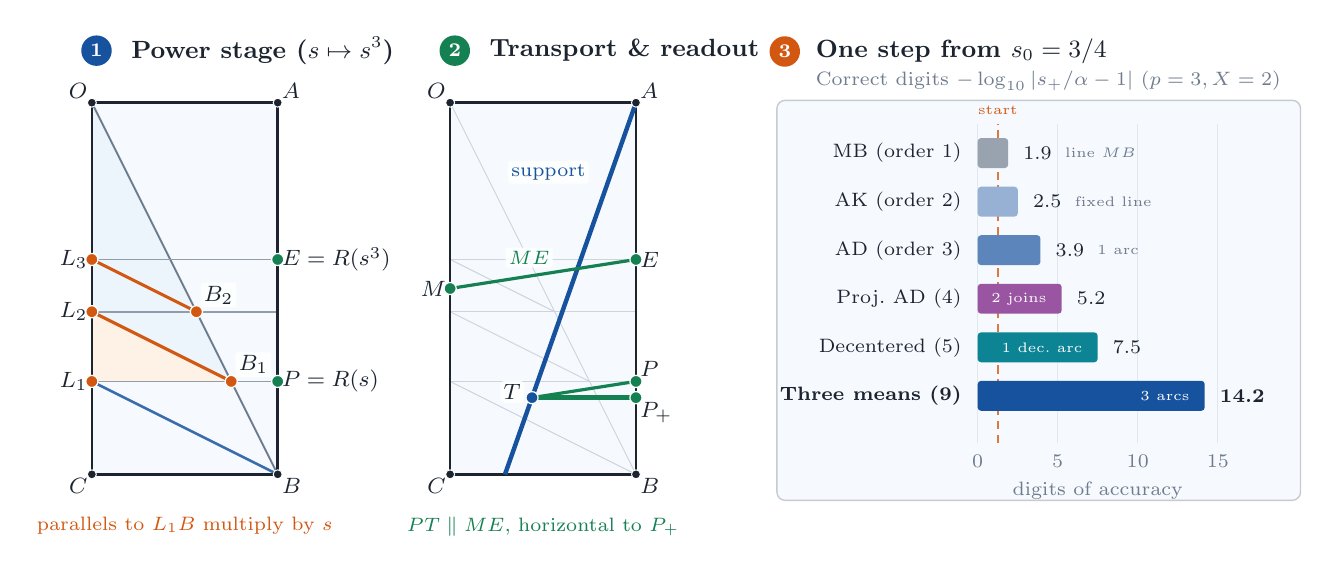
\begin{tikzpicture}
\begin{scope}[shift={(0,0)},scale=1.18]
\node[badge] at (0.05,4.560) {1};
\node[ttl] at (0.32,4.560) {Power stage ($s \mapsto s^3$)};
\fill[rectbg] (0.0000,0.0000) rectangle (2.0000,4.0000);
\fill[bluefill] (0.0000,4.0000)--(0.0000,1.0000)--(1.5000,1.0000)--cycle;
\fill[trifill] (0.0000,1.0000)--(0.0000,1.7500)--(1.5000,1.0000)--cycle;
\draw[line width=0.7pt,slatec] (0.0000,4.0000)--(2.0000,0.0000);
\draw[line width=0.9pt,supp!85] (0.0000,1.0000)--(2.0000,0.0000);
\draw[line width=0.6pt,slatec!75] (0,1.0000)--(2.0,1.0000);
\draw[line width=0.6pt,slatec!75] (0,1.7500)--(2.0,1.7500);
\draw[line width=0.6pt,slatec!75] (0,2.3125)--(2.0,2.3125);
\draw[line width=1.1pt,acc] (1.5000,1.0000)--(0.0000,1.7500);
\draw[line width=1.1pt,acc] (1.1250,1.7500)--(0.0000,2.3125);
\draw[rect] (0.0000,0.0000) rectangle (2.0000,4.0000);
\node[ptsm] at (0.0000,4.0000) {};
\node[ptsm] at (2.0000,4.0000) {};
\node[ptsm] at (0.0000,0.0000) {};
\node[ptsm] at (2.0000,0.0000) {};
\node[ptacc] at (0.0000,1.0000) {};
\node[ptacc] at (0.0000,1.7500) {};
\node[ptacc] at (0.0000,2.3125) {};
\node[ptacc] at (1.5000,1.0000) {};
\node[ptacc] at (1.1250,1.7500) {};
\node[pttrans] at (2.0000,1.0000) {};
\node[pttrans] at (2.0000,2.3125) {};
\node[labsm,above left] at (0.0000,4.0000) {$O$};
\node[labsm,above right] at (2.0000,4.0000) {$A$};
\node[labsm,below left] at (0.0000,0.0000) {$C$};
\node[labsm,below right] at (2.0000,0.0000) {$B$};
\node[labsm,left] at (0.0000,1.0000) {$L_1$};
\node[labsm,left] at (0.0000,1.7500) {$L_2$};
\node[labsm,left] at (0.0000,2.3125) {$L_3$};
\node[labsm,halo,above right] at (1.5400,1.0400) {$B_1$};
\node[labsm,halo,above right] at (1.1650,1.7900) {$B_2$};
\node[labsm,right] at (2.0000,1.0000) {$P=R(s)$};
\node[labsm,right] at (2.0000,2.3125) {$E=R(s^3)$};
\node[font=\scriptsize,text=acc,anchor=north] at (1.000,-0.35) {parallels to $L_1B$ multiply by $s$};
\end{scope}
\begin{scope}[shift={(4.55,0)},scale=1.18]
\node[badgetrans] at (0.05,4.560) {2};
\node[ttl] at (0.32,4.560) {Transport \& readout};
\fill[rectbg] (0.0000,0.0000) rectangle (2.0000,4.0000);
\draw[chainfaint] (0.0000,4.0000)--(2.0000,0.0000);
\draw[chainfaint] (0.0000,1.0000)--(2.0000,0.0000);
\draw[chainfaint] (0,1.0000)--(2.0,1.0000);
\draw[chainfaint] (0,1.7500)--(2.0,1.7500);
\draw[chainfaint] (0,2.3125)--(2.0,2.3125);
\draw[chainfaint] (1.5000,1.0000)--(0.0000,1.7500);
\draw[chainfaint] (1.1250,1.7500)--(0.0000,2.3125);
\draw[rect] (0.0000,0.0000) rectangle (2.0000,4.0000);
\draw[support] (2.0000,4.0000)--(0.5905,0.0000);
\draw[transport] (0.0000,2.0000)--(2.0000,2.3125);
\draw[transport] (2.0000,1.0000)--(0.8813,0.8252);
\draw[transport,line width=1.65pt] (0.8813,0.8252)--(2.0000,0.8252);
\node[ptsm] at (0.0000,4.0000) {};
\node[ptsm] at (2.0000,4.0000) {};
\node[ptsm] at (0.0000,0.0000) {};
\node[ptsm] at (2.0000,0.0000) {};
\node[pttrans] at (0.0000,2.0000) {};
\node[pttrans] at (2.0000,2.3125) {};
\node[pttrans] at (2.0000,1.0000) {};
\node[pttrans] at (2.0000,0.8252) {};
\node[ptsupp] at (0.8813,0.8252) {};
\node[labsm,above left] at (0.0000,4.0000) {$O$};
\node[labsm,above right] at (2.0000,4.0000) {$A$};
\node[labsm,below left] at (0.0000,0.0000) {$C$};
\node[labsm,below right] at (2.0000,0.0000) {$B$};
\node[labsm,left] at (0.0000,2.0000) {$M$};
\node[labsm,right] at (2.0000,2.3125) {$E$};
\node[labsm,above right] at (2.0000,1.0000) {$P$};
\node[labsm,below right] at (2.0000,0.8252) {$P_+$};
\node[labsm,halo,left] at (0.8013,0.8852) {$T$};
\node[font=\scriptsize,text=supp,halo,anchor=east] at (1.50,3.25) {support};
\node[font=\scriptsize,text=trans,halo,anchor=south] at (0.85,2.22) {$ME$};
\node[font=\scriptsize,text=trans,anchor=north] at (1.000,-0.35) {$PT \parallel ME$, horizontal to $P_+$};
\end{scope}
\begin{scope}[shift={(8.95,0.35)}]
\node[badgeacc] at (-0.15,5.020) {3};
\node[ttl] at (0.12,5.020) {One step from $s_0=3/4$};
\node[font=\scriptsize,text=slatec,anchor=west] at (0.12,4.650) {Correct digits $-\log_{10}|s_+/\alpha-1|$ ($p=3, X=2$)};
\draw[card] (-0.25,-0.68) rectangle (6.40,4.40);
\draw[line width=0.35pt,gridc] (2.300,0.05)--(2.300,4.100);
\node[font=\scriptsize,text=slatec] at (2.300,-0.18) {0};
\draw[line width=0.35pt,gridc] (3.317,0.05)--(3.317,4.100);
\node[font=\scriptsize,text=slatec] at (3.317,-0.18) {5};
\draw[line width=0.35pt,gridc] (4.333,0.05)--(4.333,4.100);
\node[font=\scriptsize,text=slatec] at (4.333,-0.18) {10};
\draw[line width=0.35pt,gridc] (5.350,0.05)--(5.350,4.100);
\node[font=\scriptsize,text=slatec] at (5.350,-0.18) {15};
\draw[line width=0.6pt,densely dashed,acc!80] (2.556,0.05)--(2.556,4.100);
\node[font=\tiny,text=acc,anchor=south] at (2.556,4.100) {start};
\fill[slatec!70,rounded corners=1.2pt] (2.300,3.540) rectangle (2.687,3.920);
\node[font=\scriptsize,text=ink,anchor=east] at (2.220,3.730) {MB (order 1)};
\node[font=\scriptsize,text=ink,anchor=west] at (2.757,3.730) {1.9};
\node[font=\tiny,text=slatec,anchor=west] at (3.287,3.730) {line $MB$};
\fill[supp!45,rounded corners=1.2pt] (2.300,2.923) rectangle (2.809,3.303);
\node[font=\scriptsize,text=ink,anchor=east] at (2.220,3.113) {AK (order 2)};
\node[font=\scriptsize,text=ink,anchor=west] at (2.879,3.113) {2.5};
\node[font=\tiny,text=slatec,anchor=west] at (3.409,3.113) {fixed line};
\fill[supp!70,rounded corners=1.2pt] (2.300,2.307) rectangle (3.097,2.687);
\node[font=\scriptsize,text=ink,anchor=east] at (2.220,2.497) {AD (order 3)};
\node[font=\scriptsize,text=ink,anchor=west] at (3.167,2.497) {3.9};
\node[font=\tiny,text=slatec,anchor=west] at (3.697,2.497) {1 arc};
\fill[plum!80,rounded corners=1.2pt] (2.300,1.690) rectangle (3.367,2.070);
\node[font=\scriptsize,text=ink,anchor=east] at (2.220,1.880) {Proj.\ AD (4)};
\node[font=\scriptsize,text=ink,anchor=west] at (3.437,1.880) {5.2};
\node[font=\tiny,text=white,anchor=east] at (3.297,1.880) {2 joins};
\fill[tealc,rounded corners=1.2pt] (2.300,1.073) rectangle (3.823,1.453);
\node[font=\scriptsize,text=ink,anchor=east] at (2.220,1.263) {Decentered (5)};
\node[font=\scriptsize,text=ink,anchor=west] at (3.893,1.263) {7.5};
\node[font=\tiny,text=white,anchor=east] at (3.753,1.263) {1 dec.\ arc};
\fill[supp,rounded corners=1.2pt] (2.300,0.457) rectangle (5.183,0.837);
\node[font=\scriptsize\bfseries,text=ink,anchor=east] at (2.220,0.647) {Three means (9)};
\node[font=\scriptsize\bfseries,text=ink,anchor=west] at (5.253,0.647) {14.2};
\node[font=\tiny,text=white,anchor=east] at (5.113,0.647) {3 arcs};
\node[font=\scriptsize,text=slatec,anchor=north] at (3.825,-0.32) {digits of accuracy};
\end{scope}
\end{tikzpicture}%
}

\newcommand{\figTarget}{%
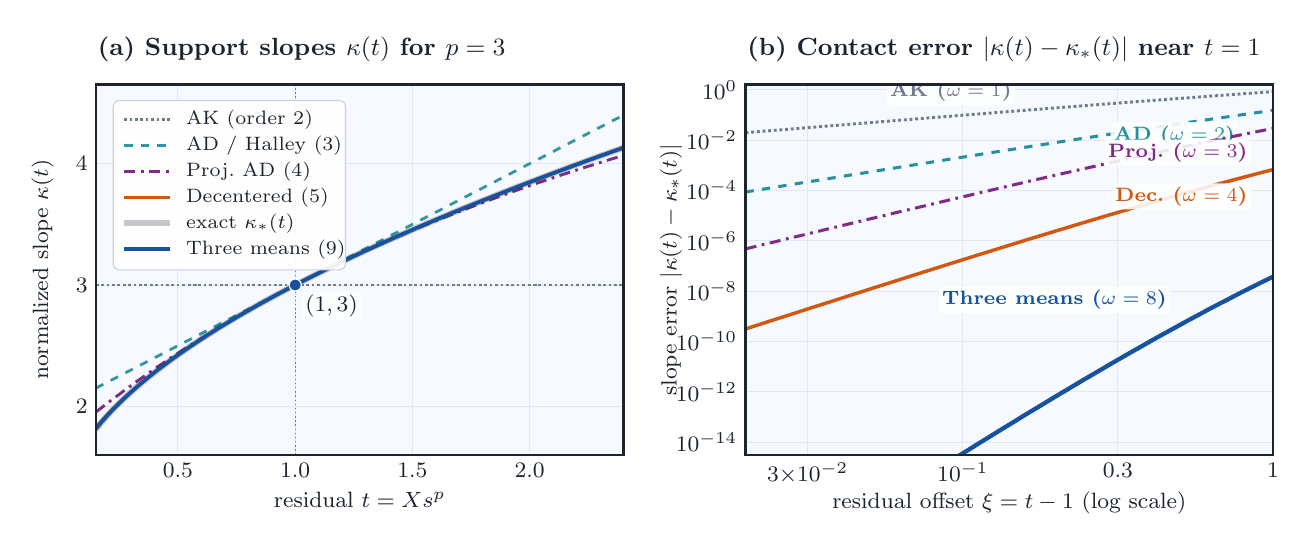
\begin{tikzpicture}
\begin{scope}[shift={(0,0)}]
\node[ttl] at (-0.1,5.150) {(a) Support slopes $\kappa(t)$ for $p=3$};
\fill[rectbg] (0,0) rectangle (6.700,4.700);
\draw[line width=0.35pt,gridc] (1.042,0)--(1.042,4.700);
\node[labsm,below] at (1.042,-0.05) {0.5};
\draw[line width=0.35pt,gridc] (2.531,0)--(2.531,4.700);
\node[labsm,below] at (2.531,-0.05) {1.0};
\draw[line width=0.35pt,gridc] (4.020,0)--(4.020,4.700);
\node[labsm,below] at (4.020,-0.05) {1.5};
\draw[line width=0.35pt,gridc] (5.509,0)--(5.509,4.700);
\node[labsm,below] at (5.509,-0.05) {2.0};
\draw[line width=0.35pt,gridc] (0,0.616)--(6.700,0.616);
\node[labsm,left] at (-0.05,0.616) {2};
\draw[line width=0.35pt,gridc] (0,2.157)--(6.700,2.157);
\node[labsm,left] at (-0.05,2.157) {3};
\draw[line width=0.35pt,gridc] (0,3.698)--(6.700,3.698);
\node[labsm,left] at (-0.05,3.698) {4};
\draw[line width=0.5pt,densely dotted,slatec] (2.531,0)--(2.531,4.700);
\begin{scope}
\clip (0,0) rectangle (6.700,4.700);
\draw[slatec,line width=0.95pt,densely dotted] (0.000,2.157)--(0.074,2.157)--(0.149,2.157)--(0.223,2.157)--(0.298,2.157)--(0.372,2.157)--(0.447,2.157)--(0.521,2.157)--(0.596,2.157)--(0.670,2.157)--(0.744,2.157)--(0.819,2.157)--(0.893,2.157)--(0.968,2.157)--(1.042,2.157)--(1.117,2.157)--(1.191,2.157)--(1.266,2.157)--(1.340,2.157)--(1.414,2.157)--(1.489,2.157)--(1.563,2.157)--(1.638,2.157)--(1.712,2.157)--(1.787,2.157)--(1.861,2.157)--(1.936,2.157)--(2.010,2.157)--(2.084,2.157)--(2.159,2.157)--(2.233,2.157)--(2.308,2.157)--(2.382,2.157)--(2.457,2.157)--(2.531,2.157)--(2.606,2.157)--(2.680,2.157)--(2.754,2.157)--(2.829,2.157)--(2.903,2.157)--(2.978,2.157)--(3.052,2.157)--(3.127,2.157)--(3.201,2.157)--(3.276,2.157)--(3.350,2.157)--(3.424,2.157)--(3.499,2.157)--(3.573,2.157)--(3.648,2.157)--(3.722,2.157)--(3.797,2.157)--(3.871,2.157)--(3.946,2.157)--(4.020,2.157)--(4.094,2.157)--(4.169,2.157)--(4.243,2.157)--(4.318,2.157)--(4.392,2.157)--(4.467,2.157)--(4.541,2.157)--(4.616,2.157)--(4.690,2.157)--(4.764,2.157)--(4.839,2.157)--(4.913,2.157)--(4.988,2.157)--(5.062,2.157)--(5.137,2.157)--(5.211,2.157)--(5.286,2.157)--(5.360,2.157)--(5.434,2.157)--(5.509,2.157)--(5.583,2.157)--(5.658,2.157)--(5.732,2.157)--(5.807,2.157)--(5.881,2.157)--(5.956,2.157)--(6.030,2.157)--(6.104,2.157)--(6.179,2.157)--(6.253,2.157)--(6.328,2.157)--(6.402,2.157)--(6.477,2.157)--(6.551,2.157)--(6.626,2.157)--(6.700,2.157);
\draw[tealc!85,line width=1.0pt,dashed] (0.000,0.848)--(0.074,0.886)--(0.149,0.925)--(0.223,0.963)--(0.298,1.002)--(0.372,1.040)--(0.447,1.079)--(0.521,1.117)--(0.596,1.156)--(0.670,1.194)--(0.744,1.233)--(0.819,1.271)--(0.893,1.310)--(0.968,1.348)--(1.042,1.387)--(1.117,1.425)--(1.191,1.464)--(1.266,1.502)--(1.340,1.541)--(1.414,1.580)--(1.489,1.618)--(1.563,1.657)--(1.638,1.695)--(1.712,1.734)--(1.787,1.772)--(1.861,1.811)--(1.936,1.849)--(2.010,1.888)--(2.084,1.926)--(2.159,1.965)--(2.233,2.003)--(2.308,2.042)--(2.382,2.080)--(2.457,2.119)--(2.531,2.157)--(2.606,2.196)--(2.680,2.234)--(2.754,2.273)--(2.829,2.311)--(2.903,2.350)--(2.978,2.389)--(3.052,2.427)--(3.127,2.466)--(3.201,2.504)--(3.276,2.543)--(3.350,2.581)--(3.424,2.620)--(3.499,2.658)--(3.573,2.697)--(3.648,2.735)--(3.722,2.774)--(3.797,2.812)--(3.871,2.851)--(3.946,2.889)--(4.020,2.928)--(4.094,2.966)--(4.169,3.005)--(4.243,3.043)--(4.318,3.082)--(4.392,3.120)--(4.467,3.159)--(4.541,3.198)--(4.616,3.236)--(4.690,3.275)--(4.764,3.313)--(4.839,3.352)--(4.913,3.390)--(4.988,3.429)--(5.062,3.467)--(5.137,3.506)--(5.211,3.544)--(5.286,3.583)--(5.360,3.621)--(5.434,3.660)--(5.509,3.698)--(5.583,3.737)--(5.658,3.775)--(5.732,3.814)--(5.807,3.852)--(5.881,3.891)--(5.956,3.930)--(6.030,3.968)--(6.104,4.007)--(6.179,4.045)--(6.253,4.084)--(6.328,4.122)--(6.402,4.161)--(6.477,4.199)--(6.551,4.238)--(6.626,4.276)--(6.700,4.315);
\draw[plum,line width=1.05pt,dash pattern=on 4pt off 2pt on 1pt off 2pt] (0.000,0.543)--(0.074,0.601)--(0.149,0.658)--(0.223,0.715)--(0.298,0.770)--(0.372,0.826)--(0.447,0.880)--(0.521,0.934)--(0.596,0.987)--(0.670,1.039)--(0.744,1.091)--(0.819,1.142)--(0.893,1.192)--(0.968,1.242)--(1.042,1.291)--(1.117,1.339)--(1.191,1.387)--(1.266,1.434)--(1.340,1.481)--(1.414,1.527)--(1.489,1.573)--(1.563,1.618)--(1.638,1.662)--(1.712,1.706)--(1.787,1.749)--(1.861,1.792)--(1.936,1.835)--(2.010,1.877)--(2.084,1.918)--(2.159,1.959)--(2.233,2.000)--(2.308,2.040)--(2.382,2.079)--(2.457,2.119)--(2.531,2.157)--(2.606,2.196)--(2.680,2.234)--(2.754,2.271)--(2.829,2.308)--(2.903,2.345)--(2.978,2.381)--(3.052,2.417)--(3.127,2.452)--(3.201,2.488)--(3.276,2.522)--(3.350,2.557)--(3.424,2.591)--(3.499,2.624)--(3.573,2.658)--(3.648,2.691)--(3.722,2.723)--(3.797,2.756)--(3.871,2.788)--(3.946,2.819)--(4.020,2.851)--(4.094,2.882)--(4.169,2.913)--(4.243,2.943)--(4.318,2.973)--(4.392,3.003)--(4.467,3.033)--(4.541,3.062)--(4.616,3.091)--(4.690,3.120)--(4.764,3.148)--(4.839,3.176)--(4.913,3.204)--(4.988,3.232)--(5.062,3.259)--(5.137,3.286)--(5.211,3.313)--(5.286,3.340)--(5.360,3.366)--(5.434,3.392)--(5.509,3.418)--(5.583,3.444)--(5.658,3.469)--(5.732,3.495)--(5.807,3.519)--(5.881,3.544)--(5.956,3.569)--(6.030,3.593)--(6.104,3.617)--(6.179,3.641)--(6.253,3.665)--(6.328,3.688)--(6.402,3.712)--(6.477,3.735)--(6.551,3.758)--(6.626,3.780)--(6.700,3.803);
\draw[acc,line width=1.15pt] (0.000,0.346)--(0.074,0.433)--(0.149,0.514)--(0.223,0.591)--(0.298,0.664)--(0.372,0.734)--(0.447,0.801)--(0.521,0.866)--(0.596,0.929)--(0.670,0.990)--(0.744,1.049)--(0.819,1.106)--(0.893,1.162)--(0.968,1.217)--(1.042,1.270)--(1.117,1.322)--(1.191,1.373)--(1.266,1.423)--(1.340,1.472)--(1.414,1.520)--(1.489,1.567)--(1.563,1.613)--(1.638,1.659)--(1.712,1.703)--(1.787,1.748)--(1.861,1.791)--(1.936,1.834)--(2.010,1.876)--(2.084,1.918)--(2.159,1.959)--(2.233,2.000)--(2.308,2.040)--(2.382,2.079)--(2.457,2.119)--(2.531,2.157)--(2.606,2.196)--(2.680,2.234)--(2.754,2.271)--(2.829,2.308)--(2.903,2.345)--(2.978,2.381)--(3.052,2.417)--(3.127,2.453)--(3.201,2.488)--(3.276,2.524)--(3.350,2.558)--(3.424,2.593)--(3.499,2.627)--(3.573,2.661)--(3.648,2.694)--(3.722,2.728)--(3.797,2.761)--(3.871,2.794)--(3.946,2.826)--(4.020,2.859)--(4.094,2.891)--(4.169,2.923)--(4.243,2.955)--(4.318,2.986)--(4.392,3.017)--(4.467,3.048)--(4.541,3.079)--(4.616,3.110)--(4.690,3.140)--(4.764,3.171)--(4.839,3.201)--(4.913,3.231)--(4.988,3.260)--(5.062,3.290)--(5.137,3.319)--(5.211,3.349)--(5.286,3.378)--(5.360,3.407)--(5.434,3.436)--(5.509,3.464)--(5.583,3.493)--(5.658,3.521)--(5.732,3.549)--(5.807,3.577)--(5.881,3.605)--(5.956,3.633)--(6.030,3.661)--(6.104,3.688)--(6.179,3.715)--(6.253,3.743)--(6.328,3.770)--(6.402,3.797)--(6.477,3.824)--(6.551,3.851)--(6.626,3.877)--(6.700,3.904);
\draw[ink,line width=2.2pt,opacity=0.25] (0.000,0.329)--(0.074,0.419)--(0.149,0.504)--(0.223,0.583)--(0.298,0.658)--(0.372,0.729)--(0.447,0.798)--(0.521,0.863)--(0.596,0.927)--(0.670,0.988)--(0.744,1.047)--(0.819,1.105)--(0.893,1.161)--(0.968,1.216)--(1.042,1.269)--(1.117,1.321)--(1.191,1.372)--(1.266,1.422)--(1.340,1.471)--(1.414,1.519)--(1.489,1.567)--(1.563,1.613)--(1.638,1.659)--(1.712,1.703)--(1.787,1.748)--(1.861,1.791)--(1.936,1.834)--(2.010,1.876)--(2.084,1.918)--(2.159,1.959)--(2.233,2.000)--(2.308,2.040)--(2.382,2.079)--(2.457,2.119)--(2.531,2.157)--(2.606,2.196)--(2.680,2.234)--(2.754,2.271)--(2.829,2.308)--(2.903,2.345)--(2.978,2.381)--(3.052,2.417)--(3.127,2.453)--(3.201,2.488)--(3.276,2.524)--(3.350,2.558)--(3.424,2.593)--(3.499,2.627)--(3.573,2.661)--(3.648,2.694)--(3.722,2.728)--(3.797,2.761)--(3.871,2.794)--(3.946,2.826)--(4.020,2.859)--(4.094,2.891)--(4.169,2.923)--(4.243,2.954)--(4.318,2.986)--(4.392,3.017)--(4.467,3.048)--(4.541,3.079)--(4.616,3.110)--(4.690,3.140)--(4.764,3.170)--(4.839,3.200)--(4.913,3.230)--(4.988,3.260)--(5.062,3.289)--(5.137,3.319)--(5.211,3.348)--(5.286,3.377)--(5.360,3.406)--(5.434,3.435)--(5.509,3.463)--(5.583,3.491)--(5.658,3.520)--(5.732,3.548)--(5.807,3.576)--(5.881,3.604)--(5.956,3.631)--(6.030,3.659)--(6.104,3.686)--(6.179,3.714)--(6.253,3.741)--(6.328,3.768)--(6.402,3.795)--(6.477,3.821)--(6.551,3.848)--(6.626,3.874)--(6.700,3.901);
\draw[supp,line width=1.35pt] (0.000,0.329)--(0.074,0.419)--(0.149,0.504)--(0.223,0.583)--(0.298,0.658)--(0.372,0.729)--(0.447,0.798)--(0.521,0.863)--(0.596,0.927)--(0.670,0.988)--(0.744,1.047)--(0.819,1.105)--(0.893,1.161)--(0.968,1.216)--(1.042,1.269)--(1.117,1.321)--(1.191,1.372)--(1.266,1.422)--(1.340,1.471)--(1.414,1.519)--(1.489,1.567)--(1.563,1.613)--(1.638,1.659)--(1.712,1.703)--(1.787,1.748)--(1.861,1.791)--(1.936,1.834)--(2.010,1.876)--(2.084,1.918)--(2.159,1.959)--(2.233,2.000)--(2.308,2.040)--(2.382,2.079)--(2.457,2.119)--(2.531,2.157)--(2.606,2.196)--(2.680,2.234)--(2.754,2.271)--(2.829,2.308)--(2.903,2.345)--(2.978,2.381)--(3.052,2.417)--(3.127,2.453)--(3.201,2.488)--(3.276,2.524)--(3.350,2.558)--(3.424,2.593)--(3.499,2.627)--(3.573,2.661)--(3.648,2.694)--(3.722,2.728)--(3.797,2.761)--(3.871,2.794)--(3.946,2.826)--(4.020,2.859)--(4.094,2.891)--(4.169,2.923)--(4.243,2.954)--(4.318,2.986)--(4.392,3.017)--(4.467,3.048)--(4.541,3.079)--(4.616,3.110)--(4.690,3.140)--(4.764,3.170)--(4.839,3.200)--(4.913,3.230)--(4.988,3.260)--(5.062,3.289)--(5.137,3.319)--(5.211,3.348)--(5.286,3.377)--(5.360,3.406)--(5.434,3.435)--(5.509,3.463)--(5.583,3.491)--(5.658,3.520)--(5.732,3.548)--(5.807,3.576)--(5.881,3.604)--(5.956,3.631)--(6.030,3.659)--(6.104,3.686)--(6.179,3.714)--(6.253,3.741)--(6.328,3.768)--(6.402,3.795)--(6.477,3.821)--(6.551,3.848)--(6.626,3.874)--(6.700,3.901);
\end{scope}
\node[ptsupp] at (2.531,2.157) {};
\node[labsm,halo,anchor=north west] at (2.611,2.077) {$(1,3)$};
\draw[rect] (0,0) rectangle (6.700,4.700);
\node[labsm,anchor=north] at (3.350,-0.42) {residual $t = Xs^p$};
\node[labsm,rotate=90,anchor=south] at (-0.48,2.350) {normalized slope $\kappa(t)$};
\fill[white,fill opacity=0.92,draw=slatec!35,rounded corners=2pt] (0.22,2.35) rectangle (3.17,4.50);
\draw[slatec,line width=0.95pt,densely dotted] (0.36,4.26)--(0.94,4.26);
\node[font=\scriptsize,text=ink,anchor=west] at (1.02,4.26) {AK (order 2)};
\draw[tealc!85,line width=1.0pt,dashed] (0.36,3.93)--(0.94,3.93);
\node[font=\scriptsize,text=ink,anchor=west] at (1.02,3.93) {AD / Halley (3)};
\draw[plum,line width=1.05pt,dash pattern=on 4pt off 2pt on 1pt off 2pt] (0.36,3.60)--(0.94,3.60);
\node[font=\scriptsize,text=ink,anchor=west] at (1.02,3.60) {Proj.\ AD (4)};
\draw[acc,line width=1.15pt] (0.36,3.27)--(0.94,3.27);
\node[font=\scriptsize,text=ink,anchor=west] at (1.02,3.27) {Decentered (5)};
\draw[ink,line width=2.2pt,opacity=0.25] (0.36,2.94)--(0.94,2.94);
\node[font=\scriptsize,text=ink,anchor=west] at (1.02,2.94) {exact $\kappa_*(t)$};
\draw[supp,line width=1.35pt] (0.36,2.61)--(0.94,2.61);
\node[font=\scriptsize,text=ink,anchor=west] at (1.02,2.61) {Three means (9)};
\end{scope}
\begin{scope}[shift={(8.250,0)}]
\node[ttl] at (-0.1,5.150) {(b) Contact error $|\kappa(t)-\kappa_*(t)|$ near $t=1$};
\fill[rectbg] (0,0) rectangle (6.700,4.700);
\draw[line width=0.35pt,gridc] (0.788,0)--(0.788,4.700);
\node[labsm,below] at (0.788,-0.05) {$3{\times}10^{-2}$};
\draw[line width=0.35pt,gridc] (2.759,0)--(2.759,4.700);
\node[labsm,below] at (2.759,-0.05) {$10^{-1}$};
\draw[line width=0.35pt,gridc] (4.729,0)--(4.729,4.700);
\node[labsm,below] at (4.729,-0.05) {$0.3$};
\draw[line width=0.35pt,gridc] (6.700,0)--(6.700,4.700);
\node[labsm,below] at (6.700,-0.05) {$1$};
\draw[line width=0.35pt,gridc] (0,0.160)--(6.700,0.160);
\node[labsm,left] at (-0.05,0.160) {$10^{-14}$};
\draw[line width=0.35pt,gridc] (0,0.799)--(6.700,0.799);
\node[labsm,left] at (-0.05,0.799) {$10^{-12}$};
\draw[line width=0.35pt,gridc] (0,1.439)--(6.700,1.439);
\node[labsm,left] at (-0.05,1.439) {$10^{-10}$};
\draw[line width=0.35pt,gridc] (0,2.078)--(6.700,2.078);
\node[labsm,left] at (-0.05,2.078) {$10^{-8}$};
\draw[line width=0.35pt,gridc] (0,2.718)--(6.700,2.718);
\node[labsm,left] at (-0.05,2.718) {$10^{-6}$};
\draw[line width=0.35pt,gridc] (0,3.357)--(6.700,3.357);
\node[labsm,left] at (-0.05,3.357) {$10^{-4}$};
\draw[line width=0.35pt,gridc] (0,3.997)--(6.700,3.997);
\node[labsm,left] at (-0.05,3.997) {$10^{-2}$};
\draw[line width=0.35pt,gridc] (0,4.636)--(6.700,4.636);
\node[labsm,left] at (-0.05,4.636) {$10^{0}$};
\begin{scope}
\clip (0,0) rectangle (6.700,4.700);
\draw[slatec,line width=1.05pt,densely dotted] (0.000,4.092)--(0.084,4.099)--(0.167,4.105)--(0.251,4.112)--(0.335,4.119)--(0.419,4.126)--(0.502,4.132)--(0.586,4.139)--(0.670,4.146)--(0.754,4.153)--(0.837,4.159)--(0.921,4.166)--(1.005,4.173)--(1.089,4.180)--(1.173,4.186)--(1.256,4.193)--(1.340,4.200)--(1.424,4.207)--(1.508,4.213)--(1.591,4.220)--(1.675,4.227)--(1.759,4.234)--(1.843,4.240)--(1.926,4.247)--(2.010,4.254)--(2.094,4.260)--(2.178,4.267)--(2.261,4.274)--(2.345,4.280)--(2.429,4.287)--(2.513,4.294)--(2.596,4.300)--(2.680,4.307)--(2.764,4.314)--(2.848,4.320)--(2.931,4.327)--(3.015,4.334)--(3.099,4.340)--(3.182,4.347)--(3.266,4.354)--(3.350,4.360)--(3.434,4.367)--(3.517,4.373)--(3.601,4.380)--(3.685,4.386)--(3.769,4.393)--(3.853,4.400)--(3.936,4.406)--(4.020,4.413)--(4.104,4.419)--(4.188,4.426)--(4.271,4.432)--(4.355,4.439)--(4.439,4.445)--(4.523,4.452)--(4.606,4.458)--(4.690,4.464)--(4.774,4.471)--(4.857,4.477)--(4.941,4.484)--(5.025,4.490)--(5.109,4.496)--(5.192,4.503)--(5.276,4.509)--(5.360,4.515)--(5.444,4.522)--(5.528,4.528)--(5.611,4.534)--(5.695,4.540)--(5.779,4.546)--(5.862,4.553)--(5.946,4.559)--(6.030,4.565)--(6.114,4.571)--(6.198,4.577)--(6.281,4.583)--(6.365,4.589)--(6.449,4.595)--(6.532,4.601)--(6.616,4.607)--(6.700,4.613);
\node[font=\scriptsize\bfseries,halo,text=slatec,anchor=east] at (3.428,4.609) {AK ($\omega=1$)};
\draw[tealc!90,line width=1.1pt,dashed] (0.000,3.339)--(0.084,3.352)--(0.167,3.366)--(0.251,3.379)--(0.335,3.393)--(0.419,3.406)--(0.502,3.420)--(0.586,3.433)--(0.670,3.447)--(0.754,3.460)--(0.837,3.474)--(0.921,3.487)--(1.005,3.501)--(1.089,3.514)--(1.173,3.528)--(1.256,3.541)--(1.340,3.555)--(1.424,3.568)--(1.508,3.581)--(1.591,3.595)--(1.675,3.608)--(1.759,3.622)--(1.843,3.635)--(1.926,3.648)--(2.010,3.662)--(2.094,3.675)--(2.178,3.689)--(2.261,3.702)--(2.345,3.715)--(2.429,3.729)--(2.513,3.742)--(2.596,3.755)--(2.680,3.769)--(2.764,3.782)--(2.848,3.795)--(2.931,3.808)--(3.015,3.822)--(3.099,3.835)--(3.182,3.848)--(3.266,3.861)--(3.350,3.874)--(3.434,3.887)--(3.517,3.901)--(3.601,3.914)--(3.685,3.927)--(3.769,3.940)--(3.853,3.953)--(3.936,3.966)--(4.020,3.979)--(4.104,3.992)--(4.188,4.005)--(4.271,4.018)--(4.355,4.031)--(4.439,4.043)--(4.523,4.056)--(4.606,4.069)--(4.690,4.082)--(4.774,4.094)--(4.857,4.107)--(4.941,4.120)--(5.025,4.132)--(5.109,4.145)--(5.192,4.158)--(5.276,4.170)--(5.360,4.182)--(5.444,4.195)--(5.528,4.207)--(5.611,4.220)--(5.695,4.232)--(5.779,4.244)--(5.862,4.256)--(5.946,4.268)--(6.030,4.280)--(6.114,4.292)--(6.198,4.304)--(6.281,4.316)--(6.365,4.328)--(6.449,4.340)--(6.532,4.352)--(6.616,4.363)--(6.700,4.375);
\node[font=\scriptsize\bfseries,halo,text=tealc!90,anchor=east] at (6.266,4.060) {AD ($\omega=2$)};
\draw[plum,line width=1.1pt,dash pattern=on 4pt off 2pt on 1pt off 2pt] (0.000,2.616)--(0.084,2.636)--(0.167,2.657)--(0.251,2.677)--(0.335,2.697)--(0.419,2.717)--(0.502,2.738)--(0.586,2.758)--(0.670,2.778)--(0.754,2.798)--(0.837,2.818)--(0.921,2.838)--(1.005,2.859)--(1.089,2.879)--(1.173,2.899)--(1.256,2.919)--(1.340,2.939)--(1.424,2.959)--(1.508,2.979)--(1.591,2.999)--(1.675,3.019)--(1.759,3.039)--(1.843,3.060)--(1.926,3.080)--(2.010,3.100)--(2.094,3.119)--(2.178,3.139)--(2.261,3.159)--(2.345,3.179)--(2.429,3.199)--(2.513,3.219)--(2.596,3.239)--(2.680,3.259)--(2.764,3.278)--(2.848,3.298)--(2.931,3.318)--(3.015,3.338)--(3.099,3.357)--(3.182,3.377)--(3.266,3.397)--(3.350,3.416)--(3.434,3.436)--(3.517,3.455)--(3.601,3.475)--(3.685,3.494)--(3.769,3.513)--(3.853,3.533)--(3.936,3.552)--(4.020,3.571)--(4.104,3.590)--(4.188,3.609)--(4.271,3.628)--(4.355,3.647)--(4.439,3.666)--(4.523,3.685)--(4.606,3.704)--(4.690,3.723)--(4.774,3.741)--(4.857,3.760)--(4.941,3.778)--(5.025,3.797)--(5.109,3.815)--(5.192,3.833)--(5.276,3.852)--(5.360,3.870)--(5.444,3.888)--(5.528,3.906)--(5.611,3.923)--(5.695,3.941)--(5.779,3.959)--(5.862,3.976)--(5.946,3.994)--(6.030,4.011)--(6.114,4.028)--(6.198,4.045)--(6.281,4.062)--(6.365,4.079)--(6.449,4.096)--(6.532,4.112)--(6.616,4.129)--(6.700,4.145);
\node[font=\scriptsize\bfseries,halo,text=plum,anchor=east] at (6.424,3.839) {Proj.\ ($\omega=3$)};
\draw[acc,line width=1.25pt] (0.000,1.599)--(0.084,1.626)--(0.167,1.653)--(0.251,1.680)--(0.335,1.707)--(0.419,1.734)--(0.502,1.760)--(0.586,1.787)--(0.670,1.814)--(0.754,1.841)--(0.837,1.868)--(0.921,1.895)--(1.005,1.922)--(1.089,1.948)--(1.173,1.975)--(1.256,2.002)--(1.340,2.029)--(1.424,2.056)--(1.508,2.082)--(1.591,2.109)--(1.675,2.136)--(1.759,2.162)--(1.843,2.189)--(1.926,2.215)--(2.010,2.242)--(2.094,2.269)--(2.178,2.295)--(2.261,2.322)--(2.345,2.348)--(2.429,2.374)--(2.513,2.401)--(2.596,2.427)--(2.680,2.453)--(2.764,2.480)--(2.848,2.506)--(2.931,2.532)--(3.015,2.558)--(3.099,2.584)--(3.182,2.610)--(3.266,2.636)--(3.350,2.662)--(3.434,2.688)--(3.517,2.714)--(3.601,2.740)--(3.685,2.765)--(3.769,2.791)--(3.853,2.816)--(3.936,2.842)--(4.020,2.867)--(4.104,2.892)--(4.188,2.918)--(4.271,2.943)--(4.355,2.968)--(4.439,2.993)--(4.523,3.018)--(4.606,3.043)--(4.690,3.067)--(4.774,3.092)--(4.857,3.116)--(4.941,3.141)--(5.025,3.165)--(5.109,3.189)--(5.192,3.213)--(5.276,3.237)--(5.360,3.261)--(5.444,3.285)--(5.528,3.308)--(5.611,3.332)--(5.695,3.355)--(5.779,3.378)--(5.862,3.401)--(5.946,3.424)--(6.030,3.447)--(6.114,3.469)--(6.198,3.492)--(6.281,3.514)--(6.365,3.536)--(6.449,3.558)--(6.532,3.580)--(6.616,3.602)--(6.700,3.623);
\node[font=\scriptsize\bfseries,halo,text=acc,anchor=east] at (6.424,3.282) {Dec.\ ($\omega=4$)};
\draw[supp,line width=1.55pt] (2.010,-0.451)--(2.094,-0.398)--(2.178,-0.345)--(2.261,-0.293)--(2.345,-0.240)--(2.429,-0.187)--(2.513,-0.135)--(2.596,-0.083)--(2.680,-0.030)--(2.764,0.022)--(2.848,0.074)--(2.931,0.126)--(3.015,0.178)--(3.099,0.230)--(3.182,0.281)--(3.266,0.333)--(3.350,0.384)--(3.434,0.435)--(3.517,0.487)--(3.601,0.538)--(3.685,0.588)--(3.769,0.639)--(3.853,0.690)--(3.936,0.740)--(4.020,0.790)--(4.104,0.840)--(4.188,0.890)--(4.271,0.940)--(4.355,0.989)--(4.439,1.038)--(4.523,1.087)--(4.606,1.136)--(4.690,1.185)--(4.774,1.233)--(4.857,1.281)--(4.941,1.329)--(5.025,1.376)--(5.109,1.424)--(5.192,1.471)--(5.276,1.518)--(5.360,1.564)--(5.444,1.610)--(5.528,1.656)--(5.611,1.702)--(5.695,1.747)--(5.779,1.792)--(5.862,1.837)--(5.946,1.881)--(6.030,1.925)--(6.114,1.968)--(6.198,2.012)--(6.281,2.055)--(6.365,2.097)--(6.449,2.139)--(6.532,2.181)--(6.616,2.222)--(6.700,2.263);
\node[font=\scriptsize\bfseries,halo,text=supp,anchor=east] at (5.399,1.967) {Three means ($\omega=8$)};
\end{scope}
\draw[rect] (0,0) rectangle (6.700,4.700);
\node[labsm,anchor=north] at (3.350,-0.42) {residual offset $\xi = t - 1$ (log scale)};
\node[labsm,rotate=90,anchor=south] at (-0.75,2.350) {slope error $|\kappa(t)-\kappa_*(t)|$};
\end{scope}
\end{tikzpicture}%
}

\newcommand{\figDecentered}{%
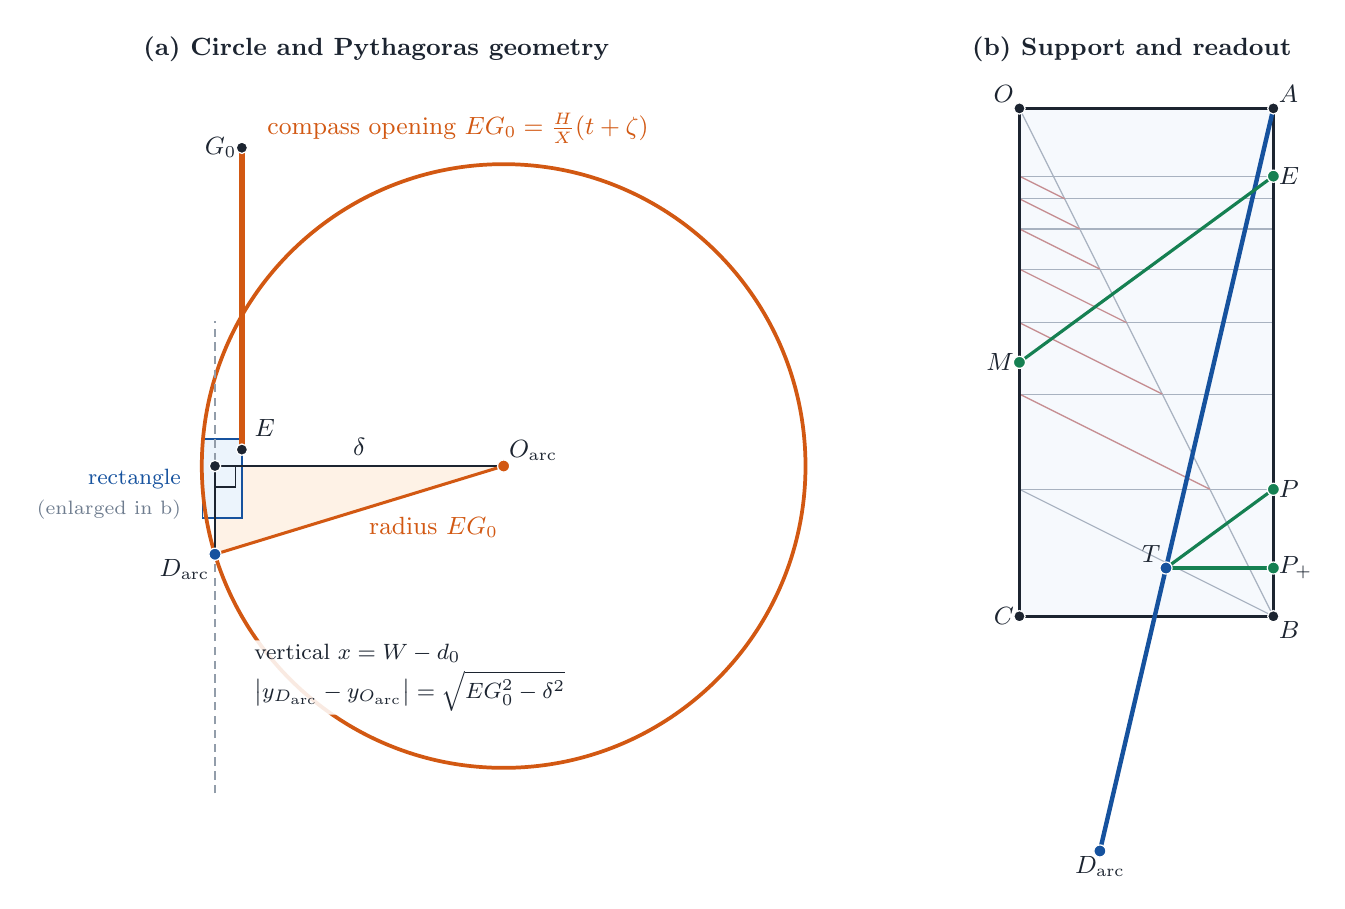
\begin{tikzpicture}[scale=0.25]
\node[ttl] at (-3.5,23.8) {(a) Circle and Pythagoras geometry};
\fill[trifill] (0.6337,-1.8484)--(0.6337,2.6337)--(15.2980,2.6337)--cycle;
\fill[bluefill] (0,0) rectangle (2.0,4.0);
\draw[line width=0.65pt,supp] (0,0) rectangle (2.0,4.0);
\draw[accent] (15.2980,2.6337) circle (15.3339);
\draw[aux] (0.6337,-14.0)--(0.6337,10.0);
\draw[accent,line width=2.4pt] (2.0000,3.4661)--(2.0000,18.8000);
\draw[line width=0.95pt,ink] (0.6337,-1.8484)--(0.6337,2.6337)--(15.2980,2.6337);
\draw[line width=1.1pt,acc] (15.2980,2.6337)--(0.6337,-1.8484);
\draw[line width=0.6pt,ink] (0.6337,1.5837)-|(1.6837,2.6337);
\node[pt] at (2.0000,18.8000) {};
\node[pt] at (2.0000,3.4661) {};
\node[pt] at (0.6337,2.6337) {};
\node[ptacc] at (15.2980,2.6337) {};
\node[ptsupp] at (0.6337,-1.8484) {};
\node[lab,left] at (2.0000,18.8000) {$G_0$};
\node[lab,halo,anchor=south west] at (2.4500,3.9161) {$E$};
\node[lab,above right] at (15.2980,2.6337) {$O_{\mathrm{arc}}$};
\node[lab,below left] at (0.6337,-1.8484) {$D_{\mathrm{arc}}$};
\node[lab,halo,text=acc,anchor=west] at (3.1000,19.8) {compass opening $EG_0=\frac HX(t+\zeta)$};
\node[lab,halo,above] at (7.9659,2.9837) {$\delta$};
\node[lab,halo,text=acc,anchor=north west] at (8.2659,0.2427) {radius $EG_0$};
\node[labsm,halo,anchor=north west,align=left] at (2.4337,-6.2) {vertical $x=W-d_0$\\[2pt]$\bigl|y_{D_{\mathrm{arc}}}-y_{O_{\mathrm{arc}}}\bigr|=\sqrt{EG_0^{2}-\delta^{2}}$};
\node[font=\footnotesize,text=supp,anchor=east] at (-0.6,2.0) {rectangle};
\node[font=\scriptsize,text=slatec,anchor=east] at (-0.6,0.4) {(enlarged in b)};
\begin{scope}[shift={(41.5,-5.0)},scale=6.45]
\node[ttl] at (-0.45,4.4651) {(b) Support and readout};
\fill[rectbg] (0.0000,0.0000) rectangle (2.0000,4.0000);
\draw[chain] (0.0000,4.0000)--(2.0000,0.0000);
\draw[chain] (0.0000,1.0000)--(2.0000,0.0000);
\draw[chain] (0,1.0000)--(2.0,1.0000);
\draw[chain] (0,1.7500)--(2.0,1.7500);
\draw[chain] (0,2.3125)--(2.0,2.3125);
\draw[chain] (0,2.7344)--(2.0,2.7344);
\draw[chain] (0,3.0508)--(2.0,3.0508);
\draw[chain] (0,3.2881)--(2.0,3.2881);
\draw[chain] (0,3.4661)--(2.0,3.4661);
\draw[chainpar] (1.5000,1.0000)--(0.0000,1.7500);
\draw[chainpar] (1.1250,1.7500)--(0.0000,2.3125);
\draw[chainpar] (0.8438,2.3125)--(0.0000,2.7344);
\draw[chainpar] (0.6328,2.7344)--(0.0000,3.0508);
\draw[chainpar] (0.4746,3.0508)--(0.0000,3.2881);
\draw[chainpar] (0.3560,3.2881)--(0.0000,3.4661);
\draw[rect] (0.0000,0.0000) rectangle (2.0000,4.0000);
\draw[support] (2.0000,4.0000)--(0.6337,-1.8484);
\draw[transport] (0.0000,2.0000)--(2.0000,3.4661);
\draw[transport] (2.0000,1.0000)--(1.1543,0.3801);
\draw[transport,line width=1.65pt] (1.1543,0.3801)--(2.0000,0.3801);
\node[lab,above left] at (0.0000,4.0000) {$O$};
\node[lab,above right] at (2.0000,4.0000) {$A$};
\node[lab,left] at (0.0000,0.0000) {$C$};
\node[lab,below right] at (2.0000,0.0000) {$B$};
\node[pt] at (0.0000,4.0000) {};
\node[pt] at (2.0000,4.0000) {};
\node[pt] at (0.0000,0.0000) {};
\node[pt] at (2.0000,0.0000) {};
\node[pttrans] at (0.0000,2.0000) {};
\node[pttrans] at (2.0000,3.4661) {};
\node[pttrans] at (2.0000,1.0000) {};
\node[ptsupp] at (1.1543,0.3801) {};
\node[pttrans] at (2.0000,0.3801) {};
\node[lab,left] at (0.0000,2.0000) {$M$};
\node[lab,right] at (2.0000,3.4661) {$E$};
\node[lab,right] at (2.0000,1.0000) {$P$};
\node[lab,right] at (2.0000,0.3801) {$P_+$};
\node[lab,above left] at (1.1543,0.3801) {$T$};
\node[ptsupp] at (0.6337,-1.8484) {};
\node[lab,below] at (0.6337,-1.8484) {$D_{\mathrm{arc}}$};
\end{scope}
\end{tikzpicture}%
}

\newcommand{\figMeanSteps}{%
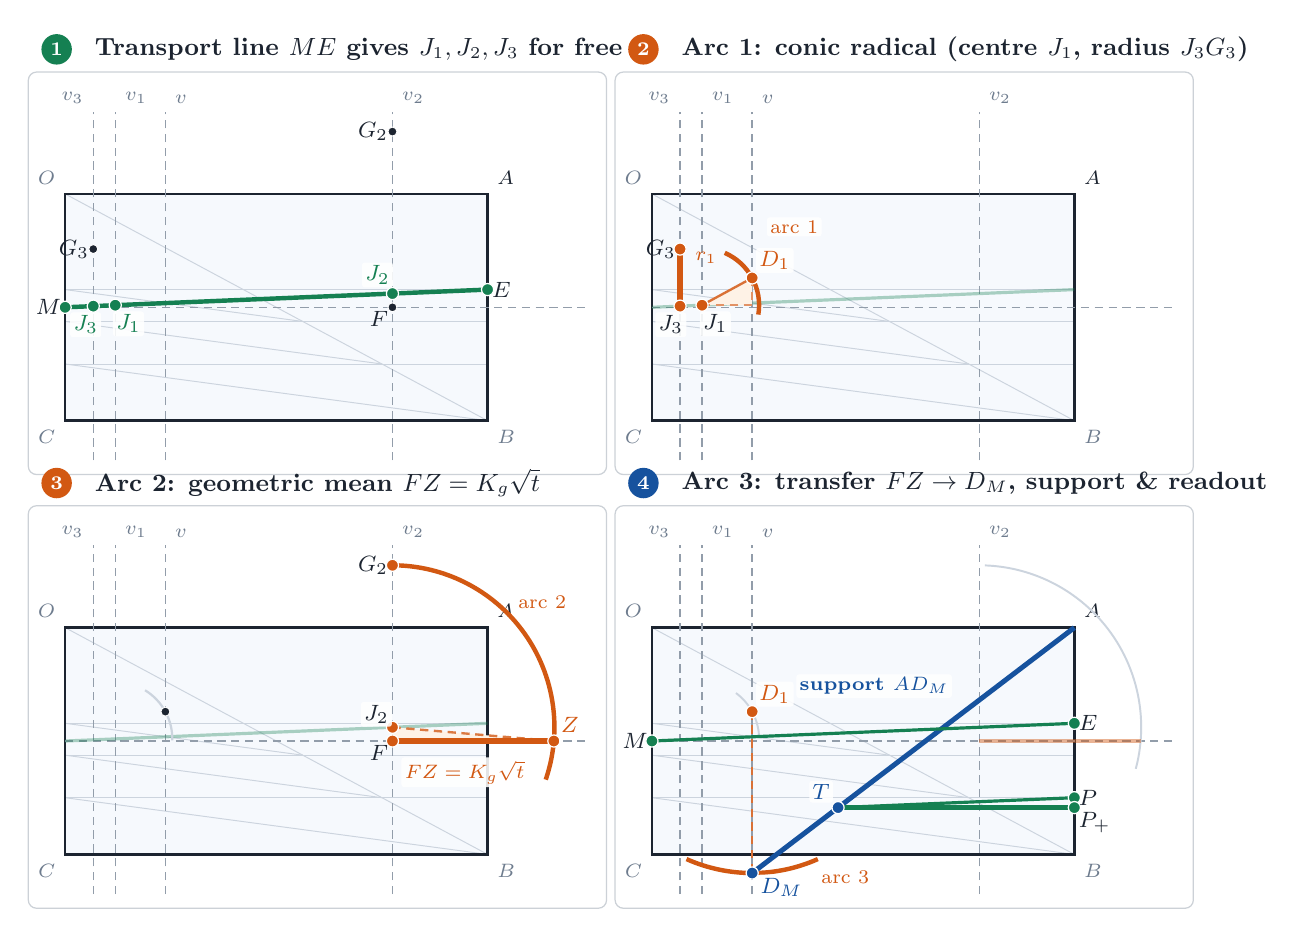
\begin{tikzpicture}[scale=0.72]
\begin{scope}[shift={(0,0)}]
\draw[line width=0.45pt,slatec!35,rounded corners=3pt,fill=white] (-0.65,-0.95) rectangle (9.55,6.15);
\fill[rectbg] (0.0000,0.0000) rectangle (7.4512,4.0000);
\draw[chainfaint] (0.0000,4.0000)--(7.4512,0.0000);
\draw[chainfaint] (0.0000,1.0000)--(7.4512,0.0000);
\draw[chainfaint] (0,1.0000)--(7.451155878422839,1.0000);
\draw[chainfaint] (0,1.7500)--(7.451155878422839,1.7500);
\draw[chainfaint] (0,2.3125)--(7.451155878422839,2.3125);
\draw[chainfaint] (5.5884,1.0000)--(0.0000,1.7500);
\draw[chainfaint] (4.1913,1.7500)--(0.0000,2.3125);
\draw[rect] (0.0000,0.0000) rectangle (7.4512,4.0000);
\draw[aux] (0.4961,-0.70)--(0.4961,5.45);
\draw[aux] (0.8840,-0.70)--(0.8840,5.45);
\draw[aux] (1.7681,-0.70)--(1.7681,5.45);
\draw[aux] (5.7733,-0.70)--(5.7733,5.45);
\draw[aux] (0,2.0000)--(9.20,2.0000);
\node[font=\scriptsize,text=slatec,anchor=south east] at (0.4961,5.42) {$v_3$};
\node[font=\scriptsize,text=slatec,anchor=south west] at (0.8840,5.42) {$v_1$};
\node[font=\scriptsize,text=slatec,anchor=south west] at (1.7681,5.42) {$v$};
\node[font=\scriptsize,text=slatec,anchor=south west] at (5.7733,5.42) {$v_2$};
\node[font=\scriptsize,text=slatec,above left] at (0.0000,4.0000) {$O$};
\node[font=\scriptsize,text=ink,above right] at (7.4512,4.0000) {$A$};
\node[font=\scriptsize,text=slatec,below left] at (0.0000,0.0000) {$C$};
\node[font=\scriptsize,text=slatec,below right] at (7.4512,0.0000) {$B$};
\node[badgetrans] at (-0.15,6.55) {1};
\node[ttl] at (0.35,6.55) {Transport line $ME$ gives $J_1, J_2, J_3$ for free};
\draw[transport,line width=1.6pt] (0.0000,2.0000)--(7.4512,2.3125);
\node[pttrans] at (0.0000,2.0000) {};
\node[pttrans] at (7.4512,2.3125) {};
\node[pttrans] at (0.8840,2.0371) {};
\node[pttrans] at (5.7733,2.2421) {};
\node[pttrans] at (0.4961,2.0208) {};
\node[ptsm] at (0.4961,3.0272) {};
\node[ptsm] at (5.7733,5.0993) {};
\node[ptsm] at (5.7733,2.0000) {};
\node[labsm,left] at (0.0000,2.0000) {$M$};
\node[labsm,right] at (7.4512,2.3125) {$E$};
\node[labsm,halo,text=trans,below left] at (0.6461,1.9208) {$J_3$};
\node[labsm,halo,text=trans,below right] at (0.8340,1.9371) {$J_1$};
\node[labsm,halo,text=trans,above left] at (5.7933,2.3421) {$J_2$};
\node[labsm,left] at (0.4961,3.0272) {$G_3$};
\node[labsm,left] at (5.7733,5.0993) {$G_2$};
\node[labsm,below left] at (5.7733,2.0000) {$F$};
\end{scope}
\begin{scope}[shift={(10.35,0)}]
\draw[line width=0.45pt,slatec!35,rounded corners=3pt,fill=white] (-0.65,-0.95) rectangle (9.55,6.15);
\fill[rectbg] (0.0000,0.0000) rectangle (7.4512,4.0000);
\draw[chainfaint] (0.0000,4.0000)--(7.4512,0.0000);
\draw[chainfaint] (0.0000,1.0000)--(7.4512,0.0000);
\draw[chainfaint] (0,1.0000)--(7.451155878422839,1.0000);
\draw[chainfaint] (0,1.7500)--(7.451155878422839,1.7500);
\draw[chainfaint] (0,2.3125)--(7.451155878422839,2.3125);
\draw[chainfaint] (5.5884,1.0000)--(0.0000,1.7500);
\draw[chainfaint] (4.1913,1.7500)--(0.0000,2.3125);
\draw[rect] (0.0000,0.0000) rectangle (7.4512,4.0000);
\draw[aux] (0.4961,-0.70)--(0.4961,5.45);
\draw[aux] (0.8840,-0.70)--(0.8840,5.45);
\draw[aux] (1.7681,-0.70)--(1.7681,5.45);
\draw[aux] (5.7733,-0.70)--(5.7733,5.45);
\draw[aux] (0,2.0000)--(9.20,2.0000);
\node[font=\scriptsize,text=slatec,anchor=south east] at (0.4961,5.42) {$v_3$};
\node[font=\scriptsize,text=slatec,anchor=south west] at (0.8840,5.42) {$v_1$};
\node[font=\scriptsize,text=slatec,anchor=south west] at (1.7681,5.42) {$v$};
\node[font=\scriptsize,text=slatec,anchor=south west] at (5.7733,5.42) {$v_2$};
\node[font=\scriptsize,text=slatec,above left] at (0.0000,4.0000) {$O$};
\node[font=\scriptsize,text=ink,above right] at (7.4512,4.0000) {$A$};
\node[font=\scriptsize,text=slatec,below left] at (0.0000,0.0000) {$C$};
\node[font=\scriptsize,text=slatec,below right] at (7.4512,0.0000) {$B$};
\node[badgeacc] at (-0.15,6.55) {2};
\node[ttl] at (0.35,6.55) {Arc 1: conic radical (centre $J_1$, radius $J_3G_3$)};
\draw[transport,opacity=0.35] (0.0000,2.0000)--(7.4512,2.3125);
\fill[trifill] (0.8840,2.0371)--(1.7681,2.0371)--(1.7681,2.5179)--cycle;
\draw[line width=0.65pt,acc!65,densely dashed] (0.8840,2.0371)--(1.7681,2.0371)--(1.7681,2.5179);
\draw[line width=0.85pt,acc!85] (0.8840,2.0371)--(1.7681,2.5179);
\draw[accent,line width=2.4pt] (0.4961,2.0208)--(0.4961,3.0272);
\draw[accent,line width=1.6pt] (0.8840,2.0371) ++(-9.46:1.0064) arc (-9.46:66.54:1.0064);
\node[ptacc] at (0.4961,2.0208) {};
\node[ptacc] at (0.4961,3.0272) {};
\node[ptacc] at (0.8840,2.0371) {};
\node[ptacc] at (1.7681,2.5179) {};
\node[labsm,left] at (0.4961,3.0272) {$G_3$};
\node[labsm,halo,below left] at (0.6161,1.9208) {$J_3$};
\node[labsm,halo,below right] at (0.8340,1.9371) {$J_1$};
\node[labsm,halo,text=acc,above right] at (1.8281,2.5979) {$D_1$};
\node[font=\scriptsize,halo,text=acc,anchor=west] at (2.0181,3.4179) {arc 1};
\node[font=\scriptsize,text=acc,anchor=west] at (0.5961,2.8740) {$r_1$};
\end{scope}
\begin{scope}[shift={(0,-7.65)}]
\draw[line width=0.45pt,slatec!35,rounded corners=3pt,fill=white] (-0.65,-0.95) rectangle (9.55,6.15);
\fill[rectbg] (0.0000,0.0000) rectangle (7.4512,4.0000);
\draw[chainfaint] (0.0000,4.0000)--(7.4512,0.0000);
\draw[chainfaint] (0.0000,1.0000)--(7.4512,0.0000);
\draw[chainfaint] (0,1.0000)--(7.451155878422839,1.0000);
\draw[chainfaint] (0,1.7500)--(7.451155878422839,1.7500);
\draw[chainfaint] (0,2.3125)--(7.451155878422839,2.3125);
\draw[chainfaint] (5.5884,1.0000)--(0.0000,1.7500);
\draw[chainfaint] (4.1913,1.7500)--(0.0000,2.3125);
\draw[rect] (0.0000,0.0000) rectangle (7.4512,4.0000);
\draw[aux] (0.4961,-0.70)--(0.4961,5.45);
\draw[aux] (0.8840,-0.70)--(0.8840,5.45);
\draw[aux] (1.7681,-0.70)--(1.7681,5.45);
\draw[aux] (5.7733,-0.70)--(5.7733,5.45);
\draw[aux] (0,2.0000)--(9.20,2.0000);
\node[font=\scriptsize,text=slatec,anchor=south east] at (0.4961,5.42) {$v_3$};
\node[font=\scriptsize,text=slatec,anchor=south west] at (0.8840,5.42) {$v_1$};
\node[font=\scriptsize,text=slatec,anchor=south west] at (1.7681,5.42) {$v$};
\node[font=\scriptsize,text=slatec,anchor=south west] at (5.7733,5.42) {$v_2$};
\node[font=\scriptsize,text=slatec,above left] at (0.0000,4.0000) {$O$};
\node[font=\scriptsize,text=ink,above right] at (7.4512,4.0000) {$A$};
\node[font=\scriptsize,text=slatec,below left] at (0.0000,0.0000) {$C$};
\node[font=\scriptsize,text=slatec,below right] at (7.4512,0.0000) {$B$};
\node[badgeacc] at (-0.15,6.55) {3};
\node[ttl] at (0.35,6.55) {Arc 2: geometric mean $FZ = K_g\sqrt{t}$};
\draw[transport,opacity=0.35] (0.0000,2.0000)--(7.4512,2.3125);
\draw[faint,line width=0.8pt] (0.8840,2.0371) ++(-1.46:1.0064) arc (-1.46:58.54:1.0064);
\fill[trifill] (5.7733,2.0000)--(5.7733,2.2421)--(8.6202,2.0000)--cycle;
\draw[line width=0.85pt,acc!80,densely dashed] (5.7733,2.2421)--(8.6202,2.0000);
\draw[accent,line width=2.4pt] (5.7733,2.0000)--(8.6202,2.0000);
\draw[accent,line width=1.6pt] (5.7733,2.2421) ++(-18.86:2.8571) arc (-18.86:90.00:2.8571);
\node[ptacc] at (5.7733,2.2421) {};
\node[ptacc] at (5.7733,5.0993) {};
\node[ptacc] at (5.7733,2.0000) {};
\node[ptacc] at (8.6202,2.0000) {};
\node[ptsm] at (1.7681,2.5179) {};
\node[labsm,left] at (5.7733,5.0993) {$G_2$};
\node[labsm,halo,above left] at (5.7733,2.2421) {$J_2$};
\node[labsm,below left] at (5.7733,2.0000) {$F$};
\node[labsm,halo,text=acc,above right] at (8.6802,2.0800) {$Z$};
\node[font=\scriptsize,halo,text=acc,anchor=north] at (7.0467,1.7200) {$FZ = K_g\sqrt{t}$};
\node[font=\scriptsize,halo,text=acc,anchor=west] at (7.9233,4.45) {arc 2};
\end{scope}
\begin{scope}[shift={(10.35,-7.65)}]
\draw[line width=0.45pt,slatec!35,rounded corners=3pt,fill=white] (-0.65,-0.95) rectangle (9.55,6.15);
\fill[rectbg] (0.0000,0.0000) rectangle (7.4512,4.0000);
\draw[chainfaint] (0.0000,4.0000)--(7.4512,0.0000);
\draw[chainfaint] (0.0000,1.0000)--(7.4512,0.0000);
\draw[chainfaint] (0,1.0000)--(7.451155878422839,1.0000);
\draw[chainfaint] (0,1.7500)--(7.451155878422839,1.7500);
\draw[chainfaint] (0,2.3125)--(7.451155878422839,2.3125);
\draw[chainfaint] (5.5884,1.0000)--(0.0000,1.7500);
\draw[chainfaint] (4.1913,1.7500)--(0.0000,2.3125);
\draw[rect] (0.0000,0.0000) rectangle (7.4512,4.0000);
\draw[aux] (0.4961,-0.70)--(0.4961,5.45);
\draw[aux] (0.8840,-0.70)--(0.8840,5.45);
\draw[aux] (1.7681,-0.70)--(1.7681,5.45);
\draw[aux] (5.7733,-0.70)--(5.7733,5.45);
\draw[aux] (0,2.0000)--(9.20,2.0000);
\node[font=\scriptsize,text=slatec,anchor=south east] at (0.4961,5.42) {$v_3$};
\node[font=\scriptsize,text=slatec,anchor=south west] at (0.8840,5.42) {$v_1$};
\node[font=\scriptsize,text=slatec,anchor=south west] at (1.7681,5.42) {$v$};
\node[font=\scriptsize,text=slatec,anchor=south west] at (5.7733,5.42) {$v_2$};
\node[font=\scriptsize,text=slatec,above left] at (0.0000,4.0000) {$O$};
\node[font=\scriptsize,text=ink,above right] at (7.4512,4.0000) {$A$};
\node[font=\scriptsize,text=slatec,below left] at (0.0000,0.0000) {$C$};
\node[font=\scriptsize,text=slatec,below right] at (7.4512,0.0000) {$B$};
\node[badge] at (-0.15,6.55) {4};
\node[ttl] at (0.35,6.55) {Arc 3: transfer $FZ \to D_M$, support \& readout};
\draw[faint,line width=0.7pt] (0.8840,2.0371) ++(3.54:1.0064) arc (3.54:53.54:1.0064);
\draw[faint,line width=0.7pt] (5.7733,2.2421) ++(-14.86:2.8571) arc (-14.86:88.00:2.8571);
\draw[accent,opacity=0.45,line width=1.6pt] (5.7733,2.0000)--(8.6202,2.0000);
\draw[line width=0.85pt,acc!85,densely dashed] (1.7681,2.5179)--(1.7681,-0.3289);
\draw[accent,line width=1.6pt] (1.7681,2.5179) ++(-114.00:2.8469) arc (-114.00:-66.00:2.8469);
\draw[support,line width=1.8pt] (7.4512,4.0000)--(1.7681,-0.3289);
\draw[transport] (0.0000,2.0000)--(7.4512,2.3125);
\draw[transport] (7.4512,1.0000)--(3.2832,0.8252);
\draw[transport,line width=1.65pt] (3.2832,0.8252)--(7.4512,0.8252);
\node[pttrans] at (0.0000,2.0000) {};
\node[pttrans] at (7.4512,2.3125) {};
\node[pttrans] at (7.4512,1.0000) {};
\node[pttrans] at (7.4512,0.8252) {};
\node[ptacc] at (1.7681,2.5179) {};
\node[ptsupp] at (1.7681,-0.3289) {};
\node[ptsupp] at (3.2832,0.8252) {};
\node[labsm,left] at (0.0000,2.0000) {$M$};
\node[labsm,right] at (7.4512,2.3125) {$E$};
\node[labsm,right] at (7.4512,1.0000) {$P$};
\node[labsm,below right] at (7.4512,0.8252) {$P_+$};
\node[labsm,halo,text=supp,above left] at (3.2032,0.9052) {$T$};
\node[labsm,halo,text=acc,above right] at (1.8281,2.5979) {$D_1$};
\node[labsm,halo,text=supp,below right] at (1.8481,-0.3489) {$D_M$};
\node[font=\scriptsize,halo,text=acc,anchor=west] at (2.9181,-0.4089) {arc 3};
\node[font=\scriptsize\bfseries,halo,text=supp,anchor=south east] at (5.30,2.75) {support $AD_M$};
\end{scope}
\end{tikzpicture}%
}

\newcommand{\figEfficiency}{%
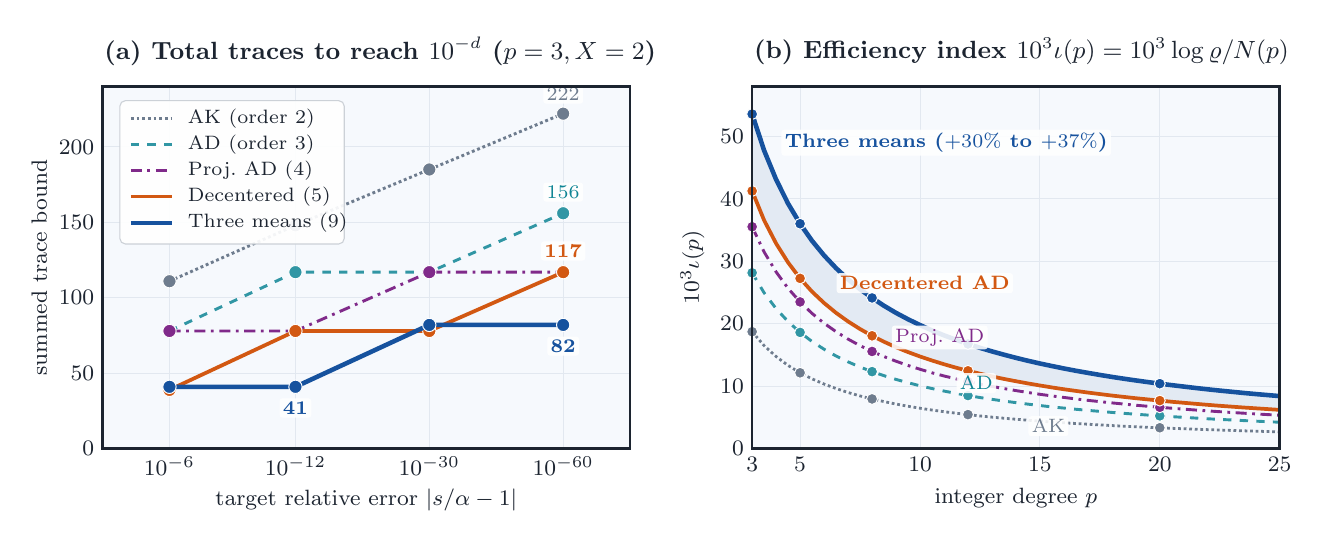
\begin{tikzpicture}
\begin{scope}[shift={(0,0)}]
\node[ttl] at (-0.1,5.050) {(a) Total traces to reach $10^{-d}$ ($p=3, X=2$)};
\fill[rectbg] (0,0) rectangle (6.700,4.600);
\draw[line width=0.35pt,gridc] (0,0.000)--(6.700,0.000);
\node[labsm,left] at (-0.05,0.000) {0};
\draw[line width=0.35pt,gridc] (0,0.958)--(6.700,0.958);
\node[labsm,left] at (-0.05,0.958) {50};
\draw[line width=0.35pt,gridc] (0,1.917)--(6.700,1.917);
\node[labsm,left] at (-0.05,1.917) {100};
\draw[line width=0.35pt,gridc] (0,2.875)--(6.700,2.875);
\node[labsm,left] at (-0.05,2.875) {150};
\draw[line width=0.35pt,gridc] (0,3.833)--(6.700,3.833);
\node[labsm,left] at (-0.05,3.833) {200};
\draw[line width=0.35pt,gridc] (0.850,0)--(0.850,4.600);
\node[labsm,below] at (0.850,-0.05) {$10^{-6}$};
\draw[line width=0.35pt,gridc] (2.450,0)--(2.450,4.600);
\node[labsm,below] at (2.450,-0.05) {$10^{-12}$};
\draw[line width=0.35pt,gridc] (4.150,0)--(4.150,4.600);
\node[labsm,below] at (4.150,-0.05) {$10^{-30}$};
\draw[line width=0.35pt,gridc] (5.850,0)--(5.850,4.600);
\node[labsm,below] at (5.850,-0.05) {$10^{-60}$};
\draw[slatec,densely dotted,line width=1.05pt] (0.850,2.127)--(2.450,2.837)--(4.150,3.546)--(5.850,4.255);
\node[circle,fill=slatec,draw=white,line width=0.35pt,inner sep=1.7pt] at (0.850,2.127) {};
\node[circle,fill=slatec,draw=white,line width=0.35pt,inner sep=1.7pt] at (2.450,2.837) {};
\node[circle,fill=slatec,draw=white,line width=0.35pt,inner sep=1.7pt] at (4.150,3.546) {};
\node[circle,fill=slatec,draw=white,line width=0.35pt,inner sep=1.7pt] at (5.850,4.255) {};
\draw[tealc!85,dashed,line width=1.05pt] (0.850,1.495)--(2.450,2.242)--(4.150,2.242)--(5.850,2.990);
\node[circle,fill=tealc!85,draw=white,line width=0.35pt,inner sep=1.7pt] at (0.850,1.495) {};
\node[circle,fill=tealc!85,draw=white,line width=0.35pt,inner sep=1.7pt] at (2.450,2.242) {};
\node[circle,fill=tealc!85,draw=white,line width=0.35pt,inner sep=1.7pt] at (4.150,2.242) {};
\node[circle,fill=tealc!85,draw=white,line width=0.35pt,inner sep=1.7pt] at (5.850,2.990) {};
\draw[plum,dash pattern=on 4pt off 2pt on 1pt off 2pt,line width=1.05pt] (0.850,1.495)--(2.450,1.495)--(4.150,2.242)--(5.850,2.242);
\node[circle,fill=plum,draw=white,line width=0.35pt,inner sep=1.7pt] at (0.850,1.495) {};
\node[circle,fill=plum,draw=white,line width=0.35pt,inner sep=1.7pt] at (2.450,1.495) {};
\node[circle,fill=plum,draw=white,line width=0.35pt,inner sep=1.7pt] at (4.150,2.242) {};
\node[circle,fill=plum,draw=white,line width=0.35pt,inner sep=1.7pt] at (5.850,2.242) {};
\draw[acc,solid,line width=1.35pt] (0.850,0.747)--(2.450,1.495)--(4.150,1.495)--(5.850,2.242);
\node[circle,fill=acc,draw=white,line width=0.35pt,inner sep=1.7pt] at (0.850,0.747) {};
\node[circle,fill=acc,draw=white,line width=0.35pt,inner sep=1.7pt] at (2.450,1.495) {};
\node[circle,fill=acc,draw=white,line width=0.35pt,inner sep=1.7pt] at (4.150,1.495) {};
\node[circle,fill=acc,draw=white,line width=0.35pt,inner sep=1.7pt] at (5.850,2.242) {};
\draw[supp,solid,line width=1.65pt] (0.850,0.786)--(2.450,0.786)--(4.150,1.572)--(5.850,1.572);
\node[circle,fill=supp,draw=white,line width=0.35pt,inner sep=1.7pt] at (0.850,0.786) {};
\node[circle,fill=supp,draw=white,line width=0.35pt,inner sep=1.7pt] at (2.450,0.786) {};
\node[circle,fill=supp,draw=white,line width=0.35pt,inner sep=1.7pt] at (4.150,1.572) {};
\node[circle,fill=supp,draw=white,line width=0.35pt,inner sep=1.7pt] at (5.850,1.572) {};
\node[font=\scriptsize\bfseries,text=supp,halo,anchor=north] at (5.850,1.432) {82};
\node[font=\scriptsize\bfseries,text=acc,halo,anchor=south] at (5.850,2.382) {117};
\node[font=\scriptsize,text=tealc,halo,anchor=south] at (5.850,3.130) {156};
\node[font=\scriptsize,text=slatec,halo,anchor=south] at (5.850,4.375) {222};
\node[font=\scriptsize\bfseries,text=supp,halo,anchor=north] at (2.450,0.646) {41};
\fill[white,fill opacity=0.92,draw=slatec!35,rounded corners=2pt] (0.22,2.60) rectangle (3.07,4.42);
\draw[slatec,densely dotted,line width=1.05pt] (0.36,4.19)--(0.88,4.19);
\node[font=\scriptsize,text=ink,anchor=west] at (0.96,4.19) {AK (order 2)};
\draw[tealc!85,dashed,line width=1.05pt] (0.36,3.86)--(0.88,3.86);
\node[font=\scriptsize,text=ink,anchor=west] at (0.96,3.86) {AD (order 3)};
\draw[plum,dash pattern=on 4pt off 2pt on 1pt off 2pt,line width=1.05pt] (0.36,3.53)--(0.88,3.53);
\node[font=\scriptsize,text=ink,anchor=west] at (0.96,3.53) {Proj.\ AD (4)};
\draw[acc,solid,line width=1.05pt] (0.36,3.20)--(0.88,3.20);
\node[font=\scriptsize,text=ink,anchor=west] at (0.96,3.20) {Decentered (5)};
\draw[supp,solid,line width=1.5pt] (0.36,2.87)--(0.88,2.87);
\node[font=\scriptsize,text=ink,anchor=west] at (0.96,2.87) {Three means (9)};
\draw[rect] (0,0) rectangle (6.700,4.600);
\node[labsm,anchor=north] at (3.350,-0.45) {target relative error $|s/\alpha-1|$};
\node[labsm,rotate=90,anchor=south] at (-0.65,2.300) {summed trace bound};
\end{scope}
\begin{scope}[shift={(8.250,0)}]
\node[ttl] at (-0.1,5.050) {(b) Efficiency index $10^3\iota(p)=10^3\log\varrho/N(p)$};
\fill[rectbg] (0,0) rectangle (6.700,4.600);
\draw[line width=0.35pt,gridc] (0.000,0)--(0.000,4.600);
\node[labsm,below] at (0.000,-0.05) {3};
\draw[line width=0.35pt,gridc] (0.609,0)--(0.609,4.600);
\node[labsm,below] at (0.609,-0.05) {5};
\draw[line width=0.35pt,gridc] (2.132,0)--(2.132,4.600);
\node[labsm,below] at (2.132,-0.05) {10};
\draw[line width=0.35pt,gridc] (3.655,0)--(3.655,4.600);
\node[labsm,below] at (3.655,-0.05) {15};
\draw[line width=0.35pt,gridc] (5.177,0)--(5.177,4.600);
\node[labsm,below] at (5.177,-0.05) {20};
\draw[line width=0.35pt,gridc] (6.700,0)--(6.700,4.600);
\node[labsm,below] at (6.700,-0.05) {25};
\draw[line width=0.35pt,gridc] (0,0.000)--(6.700,0.000);
\node[labsm,left] at (-0.05,0.000) {0};
\draw[line width=0.35pt,gridc] (0,0.793)--(6.700,0.793);
\node[labsm,left] at (-0.05,0.793) {10};
\draw[line width=0.35pt,gridc] (0,1.586)--(6.700,1.586);
\node[labsm,left] at (-0.05,1.586) {20};
\draw[line width=0.35pt,gridc] (0,2.379)--(6.700,2.379);
\node[labsm,left] at (-0.05,2.379) {30};
\draw[line width=0.35pt,gridc] (0,3.172)--(6.700,3.172);
\node[labsm,left] at (-0.05,3.172) {40};
\draw[line width=0.35pt,gridc] (0,3.966)--(6.700,3.966);
\node[labsm,left] at (-0.05,3.966) {50};
\fill[supp!12] (0.000,4.250)--(0.152,3.788)--(0.305,3.417)--(0.457,3.112)--(0.609,2.857)--(0.761,2.640)--(0.914,2.454)--(1.066,2.293)--(1.218,2.151)--(1.370,2.026)--(1.523,1.915)--(1.675,1.815)--(1.827,1.725)--(1.980,1.644)--(2.132,1.570)--(2.284,1.502)--(2.436,1.440)--(2.589,1.383)--(2.741,1.330)--(2.893,1.281)--(3.045,1.236)--(3.198,1.194)--(3.350,1.154)--(3.502,1.117)--(3.655,1.082)--(3.807,1.050)--(3.959,1.019)--(4.111,0.990)--(4.264,0.963)--(4.416,0.937)--(4.568,0.912)--(4.720,0.889)--(4.873,0.867)--(5.025,0.846)--(5.177,0.826)--(5.330,0.807)--(5.482,0.789)--(5.634,0.771)--(5.786,0.754)--(5.939,0.738)--(6.091,0.723)--(6.243,0.708)--(6.395,0.694)--(6.548,0.681)--(6.700,0.668)--(6.700,0.493)--(6.548,0.503)--(6.395,0.513)--(6.243,0.523)--(6.091,0.534)--(5.939,0.545)--(5.786,0.557)--(5.634,0.570)--(5.482,0.583)--(5.330,0.596)--(5.177,0.611)--(5.025,0.626)--(4.873,0.641)--(4.720,0.658)--(4.568,0.675)--(4.416,0.694)--(4.264,0.713)--(4.111,0.734)--(3.959,0.755)--(3.807,0.778)--(3.655,0.803)--(3.502,0.829)--(3.350,0.857)--(3.198,0.886)--(3.045,0.918)--(2.893,0.953)--(2.741,0.989)--(2.589,1.029)--(2.436,1.073)--(2.284,1.120)--(2.132,1.171)--(1.980,1.227)--(1.827,1.289)--(1.675,1.358)--(1.523,1.434)--(1.370,1.520)--(1.218,1.616)--(1.066,1.725)--(0.914,1.850)--(0.761,1.994)--(0.609,2.163)--(0.457,2.364)--(0.305,2.605)--(0.152,2.901)--(0.000,3.273)--cycle;
\draw[slatec,densely dotted,line width=1.0pt] (0.000,1.486)--(0.152,1.309)--(0.305,1.170)--(0.457,1.057)--(0.609,0.964)--(0.761,0.887)--(0.914,0.821)--(1.066,0.764)--(1.218,0.714)--(1.370,0.670)--(1.523,0.632)--(1.675,0.598)--(1.827,0.567)--(1.980,0.539)--(2.132,0.514)--(2.284,0.491)--(2.436,0.470)--(2.589,0.451)--(2.741,0.433)--(2.893,0.416)--(3.045,0.401)--(3.198,0.387)--(3.350,0.374)--(3.502,0.362)--(3.655,0.350)--(3.807,0.339)--(3.959,0.329)--(4.111,0.320)--(4.264,0.311)--(4.416,0.302)--(4.568,0.294)--(4.720,0.286)--(4.873,0.279)--(5.025,0.272)--(5.177,0.266)--(5.330,0.259)--(5.482,0.253)--(5.634,0.248)--(5.786,0.242)--(5.939,0.237)--(6.091,0.232)--(6.243,0.227)--(6.395,0.223)--(6.548,0.218)--(6.700,0.214);
\node[circle,fill=slatec,draw=white,line width=0.35pt,inner sep=1.4pt] at (0.000,1.486) {};
\node[circle,fill=slatec,draw=white,line width=0.35pt,inner sep=1.4pt] at (0.609,0.964) {};
\node[circle,fill=slatec,draw=white,line width=0.35pt,inner sep=1.4pt] at (1.523,0.632) {};
\node[circle,fill=slatec,draw=white,line width=0.35pt,inner sep=1.4pt] at (2.741,0.433) {};
\node[circle,fill=slatec,draw=white,line width=0.35pt,inner sep=1.4pt] at (5.177,0.266) {};
\draw[tealc!85,dashed,line width=1.05pt] (0.000,2.234)--(0.152,1.980)--(0.305,1.778)--(0.457,1.614)--(0.609,1.477)--(0.761,1.361)--(0.914,1.263)--(1.066,1.177)--(1.218,1.103)--(1.370,1.037)--(1.523,0.979)--(1.675,0.927)--(1.827,0.880)--(1.980,0.838)--(2.132,0.799)--(2.284,0.764)--(2.436,0.732)--(2.589,0.703)--(2.741,0.675)--(2.893,0.650)--(3.045,0.627)--(3.198,0.605)--(3.350,0.585)--(3.502,0.566)--(3.655,0.548)--(3.807,0.531)--(3.959,0.516)--(4.111,0.501)--(4.264,0.487)--(4.416,0.474)--(4.568,0.461)--(4.720,0.449)--(4.873,0.438)--(5.025,0.427)--(5.177,0.417)--(5.330,0.407)--(5.482,0.398)--(5.634,0.389)--(5.786,0.380)--(5.939,0.372)--(6.091,0.365)--(6.243,0.357)--(6.395,0.350)--(6.548,0.343)--(6.700,0.336);
\node[circle,fill=tealc!85,draw=white,line width=0.35pt,inner sep=1.4pt] at (0.000,2.234) {};
\node[circle,fill=tealc!85,draw=white,line width=0.35pt,inner sep=1.4pt] at (0.609,1.477) {};
\node[circle,fill=tealc!85,draw=white,line width=0.35pt,inner sep=1.4pt] at (1.523,0.979) {};
\node[circle,fill=tealc!85,draw=white,line width=0.35pt,inner sep=1.4pt] at (2.741,0.675) {};
\node[circle,fill=tealc!85,draw=white,line width=0.35pt,inner sep=1.4pt] at (5.177,0.417) {};
\draw[plum,dash pattern=on 4pt off 2pt on 1pt off 2pt,line width=1.05pt] (0.000,2.819)--(0.152,2.499)--(0.305,2.244)--(0.457,2.036)--(0.609,1.864)--(0.761,1.718)--(0.914,1.593)--(1.066,1.486)--(1.218,1.392)--(1.370,1.309)--(1.523,1.235)--(1.675,1.170)--(1.827,1.111)--(1.980,1.057)--(2.132,1.009)--(2.284,0.964)--(2.436,0.924)--(2.589,0.887)--(2.741,0.852)--(2.893,0.821)--(3.045,0.791)--(3.198,0.764)--(3.350,0.738)--(3.502,0.714)--(3.655,0.691)--(3.807,0.670)--(3.959,0.651)--(4.111,0.632)--(4.264,0.614)--(4.416,0.598)--(4.568,0.582)--(4.720,0.567)--(4.873,0.552)--(5.025,0.539)--(5.177,0.526)--(5.330,0.514)--(5.482,0.502)--(5.634,0.491)--(5.786,0.480)--(5.939,0.470)--(6.091,0.460)--(6.243,0.451)--(6.395,0.442)--(6.548,0.433)--(6.700,0.425);
\node[circle,fill=plum,draw=white,line width=0.35pt,inner sep=1.4pt] at (0.000,2.819) {};
\node[circle,fill=plum,draw=white,line width=0.35pt,inner sep=1.4pt] at (0.609,1.864) {};
\node[circle,fill=plum,draw=white,line width=0.35pt,inner sep=1.4pt] at (1.523,1.235) {};
\node[circle,fill=plum,draw=white,line width=0.35pt,inner sep=1.4pt] at (2.741,0.852) {};
\node[circle,fill=plum,draw=white,line width=0.35pt,inner sep=1.4pt] at (5.177,0.526) {};
\draw[acc,solid,line width=1.35pt] (0.000,3.273)--(0.152,2.901)--(0.305,2.605)--(0.457,2.364)--(0.609,2.163)--(0.761,1.994)--(0.914,1.850)--(1.066,1.725)--(1.218,1.616)--(1.370,1.520)--(1.523,1.434)--(1.675,1.358)--(1.827,1.289)--(1.980,1.227)--(2.132,1.171)--(2.284,1.120)--(2.436,1.073)--(2.589,1.029)--(2.741,0.989)--(2.893,0.953)--(3.045,0.918)--(3.198,0.886)--(3.350,0.857)--(3.502,0.829)--(3.655,0.803)--(3.807,0.778)--(3.959,0.755)--(4.111,0.734)--(4.264,0.713)--(4.416,0.694)--(4.568,0.675)--(4.720,0.658)--(4.873,0.641)--(5.025,0.626)--(5.177,0.611)--(5.330,0.596)--(5.482,0.583)--(5.634,0.570)--(5.786,0.557)--(5.939,0.545)--(6.091,0.534)--(6.243,0.523)--(6.395,0.513)--(6.548,0.503)--(6.700,0.493);
\node[circle,fill=acc,draw=white,line width=0.35pt,inner sep=1.4pt] at (0.000,3.273) {};
\node[circle,fill=acc,draw=white,line width=0.35pt,inner sep=1.4pt] at (0.609,2.163) {};
\node[circle,fill=acc,draw=white,line width=0.35pt,inner sep=1.4pt] at (1.523,1.434) {};
\node[circle,fill=acc,draw=white,line width=0.35pt,inner sep=1.4pt] at (2.741,0.989) {};
\node[circle,fill=acc,draw=white,line width=0.35pt,inner sep=1.4pt] at (5.177,0.611) {};
\draw[supp,solid,line width=1.65pt] (0.000,4.250)--(0.152,3.788)--(0.305,3.417)--(0.457,3.112)--(0.609,2.857)--(0.761,2.640)--(0.914,2.454)--(1.066,2.293)--(1.218,2.151)--(1.370,2.026)--(1.523,1.915)--(1.675,1.815)--(1.827,1.725)--(1.980,1.644)--(2.132,1.570)--(2.284,1.502)--(2.436,1.440)--(2.589,1.383)--(2.741,1.330)--(2.893,1.281)--(3.045,1.236)--(3.198,1.194)--(3.350,1.154)--(3.502,1.117)--(3.655,1.082)--(3.807,1.050)--(3.959,1.019)--(4.111,0.990)--(4.264,0.963)--(4.416,0.937)--(4.568,0.912)--(4.720,0.889)--(4.873,0.867)--(5.025,0.846)--(5.177,0.826)--(5.330,0.807)--(5.482,0.789)--(5.634,0.771)--(5.786,0.754)--(5.939,0.738)--(6.091,0.723)--(6.243,0.708)--(6.395,0.694)--(6.548,0.681)--(6.700,0.668);
\node[circle,fill=supp,draw=white,line width=0.35pt,inner sep=1.4pt] at (0.000,4.250) {};
\node[circle,fill=supp,draw=white,line width=0.35pt,inner sep=1.4pt] at (0.609,2.857) {};
\node[circle,fill=supp,draw=white,line width=0.35pt,inner sep=1.4pt] at (1.523,1.915) {};
\node[circle,fill=supp,draw=white,line width=0.35pt,inner sep=1.4pt] at (2.741,1.330) {};
\node[circle,fill=supp,draw=white,line width=0.35pt,inner sep=1.4pt] at (5.177,0.826) {};
\node[font=\scriptsize\bfseries,text=supp,halo,anchor=west] at (0.365,3.886) {Three means ($+30\%$ to $+37\%$)};
\node[font=\scriptsize\bfseries,text=acc,halo,anchor=west] at (1.066,2.102) {Decentered AD};
\node[font=\scriptsize,text=plum,halo,anchor=west] at (1.766,1.412) {Proj.\ AD};
\node[font=\scriptsize,text=tealc,halo,anchor=west] at (2.589,0.833) {AD};
\node[font=\scriptsize,text=slatec,halo,anchor=west] at (3.502,0.286) {AK};
\draw[rect] (0,0) rectangle (6.700,4.600);
\node[labsm,anchor=north] at (3.350,-0.45) {integer degree $p$};
\node[labsm,rotate=90,anchor=south] at (-0.55,2.300) {$10^3\iota(p)$};
\end{scope}
\end{tikzpicture}%
}

\newcommand{\figSubdivision}{%
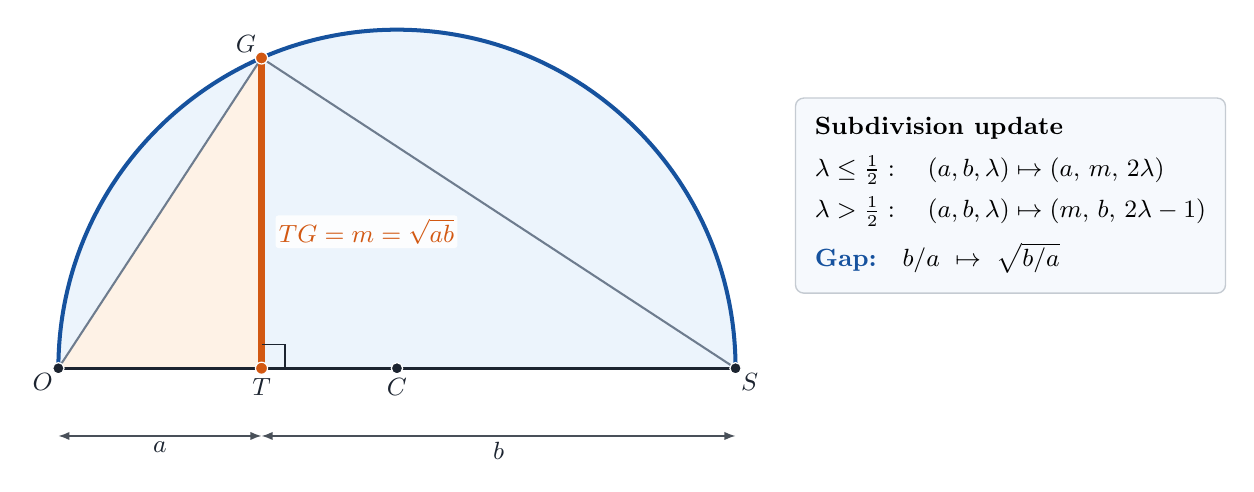
\begin{tikzpicture}[scale=2.15]
\fill[bluefill] (0,0)--(4.0,0) arc (0:180:2.0)--cycle;
\fill[trifill] (0,0)--(1.2,0)--(1.2,1.8330)--cycle;
\draw[line width=1.45pt,supp] (4.0,0) arc (0:180:2.0);
\draw[rect] (0,0)--(4.0,0);
\draw[line width=0.75pt,slatec] (0,0)--(1.2,1.8330)--(4.0,0);
\draw[accent,line width=2.2pt] (1.2,0)--(1.2,1.8330);
\draw[line width=0.55pt,ink] (1.3400,0)|-(1.2000,0.14);
\node[pt] at (0.0000,0.0000) {};
\node[pt] at (2.0000,0.0000) {};
\node[pt] at (4.0000,0.0000) {};
\node[ptacc] at (1.2,0) {};
\node[ptacc] at (1.2,1.8330) {};
\node[lab,below left] at (0,0) {$O$};
\node[lab,below] at (1.2,-0.03) {$T$};
\node[lab,below] at (2.0,-0.03) {$C$};
\node[lab,below right] at (4.0,0) {$S$};
\node[lab,above left] at (1.2,1.8330) {$G$};
\node[lab,halo,text=acc,anchor=west] at (1.28,0.8065) {$TG=m=\sqrt{ab}$};
\draw[dim] (0,-0.40)--(1.2,-0.40) node[midway,below,lab] {$a$};
\draw[dim] (1.2,-0.40)--(4.0,-0.40) node[midway,below,lab] {$b$};
\node[card,anchor=west,align=left,font=\small,inner sep=7pt] at (4.35,1.02) {\textbf{Subdivision update}\\[4pt]$\lambda\le\tfrac12:\quad (a,b,\lambda)\mapsto(a,\,m,\,2\lambda)$\\[4pt]$\lambda>\tfrac12:\quad (a,b,\lambda)\mapsto(m,\,b,\,2\lambda-1)$\\[5pt]\textcolor{supp}{\textbf{Gap:}}\quad $b/a\ \mapsto\ \sqrt{b/a}$};
\end{tikzpicture}%
}

\newcommand{\figDepth}{%
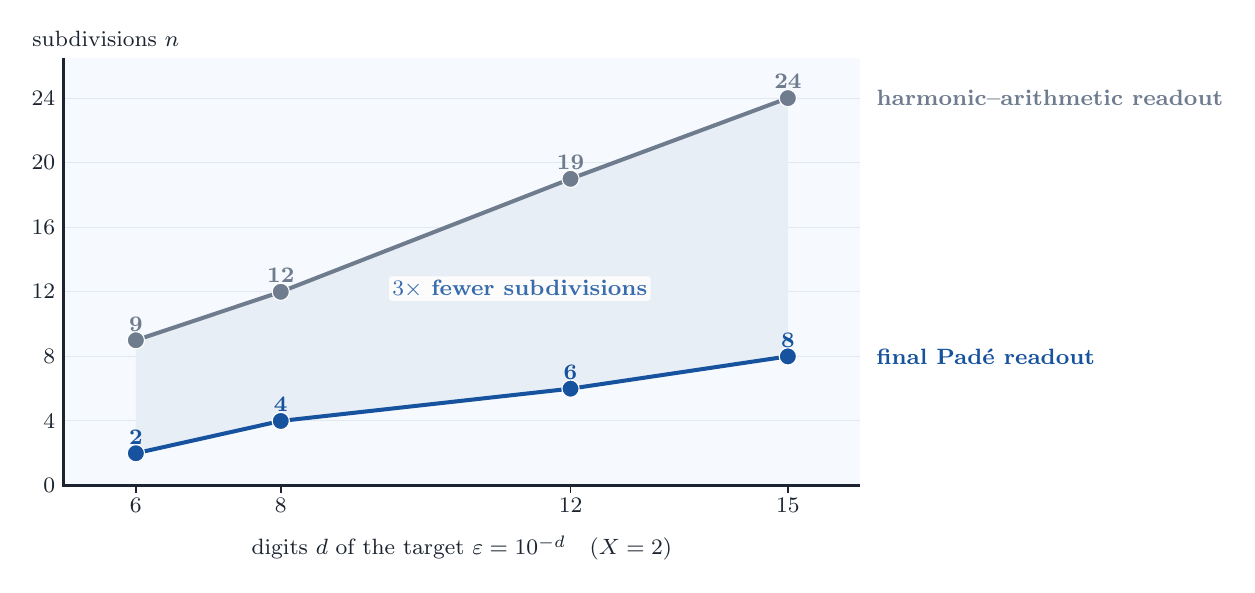
\begin{tikzpicture}
\fill[rectbg] (0,0) rectangle (10.120,5.433);
\draw[line width=0.35pt,gridc] (0,0.000)--(10.120,0.000);
\node[labsm,left] at (-0.05,0.000) {0};
\draw[line width=0.35pt,gridc] (0,0.820)--(10.120,0.820);
\node[labsm,left] at (-0.05,0.820) {4};
\draw[line width=0.35pt,gridc] (0,1.640)--(10.120,1.640);
\node[labsm,left] at (-0.05,1.640) {8};
\draw[line width=0.35pt,gridc] (0,2.460)--(10.120,2.460);
\node[labsm,left] at (-0.05,2.460) {12};
\draw[line width=0.35pt,gridc] (0,3.280)--(10.120,3.280);
\node[labsm,left] at (-0.05,3.280) {16};
\draw[line width=0.35pt,gridc] (0,4.100)--(10.120,4.100);
\node[labsm,left] at (-0.05,4.100) {20};
\draw[line width=0.35pt,gridc] (0,4.920)--(10.120,4.920);
\node[labsm,left] at (-0.05,4.920) {24};
\fill[supp!10] (0.920,1.845)--(2.760,2.460)--(6.440,3.895)--(9.200,4.920)--(9.200,1.640)--(6.440,1.230)--(2.760,0.820)--(0.920,0.410)--cycle;
\node[font=\footnotesize\bfseries,text=supp!85,halo] at (5.796,2.501) {$3\times$ fewer subdivisions};
\draw[rect] (0,5.433)--(0,0)--(10.120,0);
\draw[line width=0.6pt,ink] (0.920,0)--(0.920,-0.1);
\node[labsm,below] at (0.920,-0.1) {6};
\draw[line width=0.6pt,ink] (2.760,0)--(2.760,-0.1);
\node[labsm,below] at (2.760,-0.1) {8};
\draw[line width=0.6pt,ink] (6.440,0)--(6.440,-0.1);
\node[labsm,below] at (6.440,-0.1) {12};
\draw[line width=0.6pt,ink] (9.200,0)--(9.200,-0.1);
\node[labsm,below] at (9.200,-0.1) {15};
\draw[line width=1.45pt,slatec] (0.920,1.845)--(2.760,2.460)--(6.440,3.895)--(9.200,4.920);
\node[circle,fill=slatec,draw=white,line width=0.4pt,inner sep=2.2pt] at (0.920,1.845) {};
\node[labsm,above,slatec] at (0.920,1.905) {\textbf{9}};
\node[circle,fill=slatec,draw=white,line width=0.4pt,inner sep=2.2pt] at (2.760,2.460) {};
\node[labsm,above,slatec] at (2.760,2.520) {\textbf{12}};
\node[circle,fill=slatec,draw=white,line width=0.4pt,inner sep=2.2pt] at (6.440,3.895) {};
\node[labsm,above,slatec] at (6.440,3.955) {\textbf{19}};
\node[circle,fill=slatec,draw=white,line width=0.4pt,inner sep=2.2pt] at (9.200,4.920) {};
\node[labsm,above,slatec] at (9.200,4.980) {\textbf{24}};
\node[labsm,slatec,anchor=west] at (10.270,4.920) {\textbf{harmonic--arithmetic readout}};
\draw[line width=1.45pt,supp] (0.920,0.410)--(2.760,0.820)--(6.440,1.230)--(9.200,1.640);
\node[circle,fill=supp,draw=white,line width=0.4pt,inner sep=2.2pt] at (0.920,0.410) {};
\node[labsm,above,supp] at (0.920,0.470) {\textbf{2}};
\node[circle,fill=supp,draw=white,line width=0.4pt,inner sep=2.2pt] at (2.760,0.820) {};
\node[labsm,above,supp] at (2.760,0.880) {\textbf{4}};
\node[circle,fill=supp,draw=white,line width=0.4pt,inner sep=2.2pt] at (6.440,1.230) {};
\node[labsm,above,supp] at (6.440,1.290) {\textbf{6}};
\node[circle,fill=supp,draw=white,line width=0.4pt,inner sep=2.2pt] at (9.200,1.640) {};
\node[labsm,above,supp] at (9.200,1.700) {\textbf{8}};
\node[labsm,supp,anchor=west] at (10.270,1.640) {\textbf{final Pad\'e readout}};
\node[labsm,anchor=south west] at (-0.45,5.514) {subdivisions $n$};
\node[labsm,anchor=north] at (5.060,-0.58) {digits $d$ of the target $\varepsilon=10^{-d}$\quad($X=2$)};
\end{tikzpicture}%
}

\newcommand{\figAK}{%
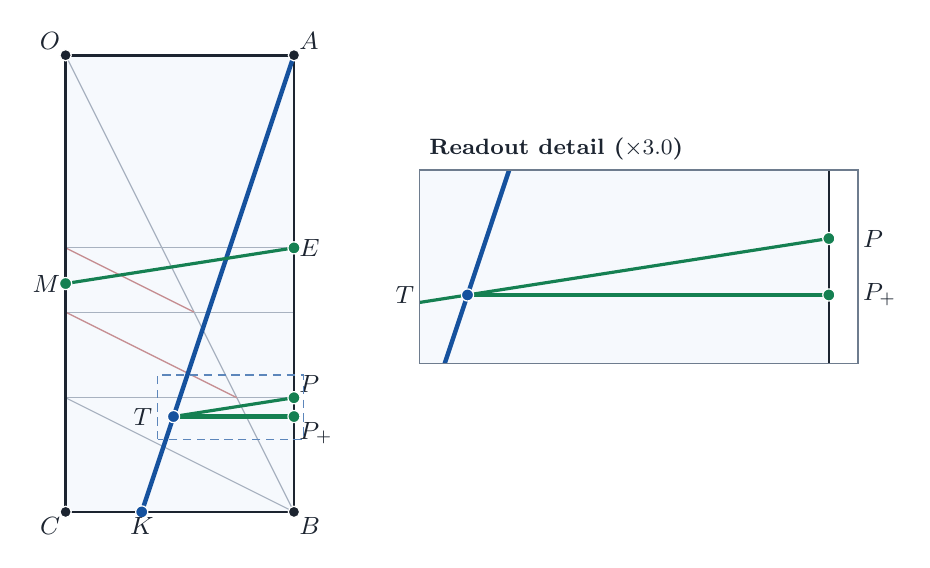
\begin{tikzpicture}[scale=1.45]
\fill[rectbg] (0.0000,0.0000) rectangle (2.0000,4.0000);
\draw[chain] (0.0000,4.0000)--(2.0000,0.0000);
\draw[chain] (0.0000,1.0000)--(2.0000,0.0000);
\draw[chain] (0,1.0000)--(2.0,1.0000);
\draw[chain] (0,1.7500)--(2.0,1.7500);
\draw[chain] (0,2.3125)--(2.0,2.3125);
\draw[chainpar] (1.5000,1.0000)--(0.0000,1.7500);
\draw[chainpar] (1.1250,1.7500)--(0.0000,2.3125);
\draw[rect] (0.0000,0.0000) rectangle (2.0000,4.0000);
\draw[support] (2.0000,4.0000)--(0.6667,0.0000);
\draw[transport] (0.0000,2.0000)--(2.0000,2.3125);
\draw[transport] (2.0000,1.0000)--(0.9451,0.8352);
\draw[transport,line width=1.65pt] (0.9451,0.8352)--(2.0000,0.8352);
\node[lab,above left] at (0.0000,4.0000) {$O$};
\node[lab,above right] at (2.0000,4.0000) {$A$};
\node[lab,below left] at (0.0000,0.0000) {$C$};
\node[lab,below right] at (2.0000,0.0000) {$B$};
\node[pt] at (0.0000,4.0000) {};
\node[pt] at (2.0000,4.0000) {};
\node[pt] at (0.0000,0.0000) {};
\node[pt] at (2.0000,0.0000) {};
\node[pttrans] at (0.0000,2.0000) {};
\node[pttrans] at (2.0000,2.3125) {};
\node[pttrans] at (2.0000,1.0000) {};
\node[ptsupp] at (0.9451,0.8352) {};
\node[pttrans] at (2.0000,0.8352) {};
\node[lab,left] at (0.0000,2.0000) {$M$};
\node[lab,right] at (2.0000,2.3125) {$E$};
\node[lab,above right] at (2.0000,1.0000) {$P$};
\node[lab,below right] at (2.0000,0.8352) {$P_+$};
\node[ptsupp] at (0.6667,0.0000) {};
\node[lab,below] at (0.6667,0.0000) {$K$};
\draw[aux,supp!70] (0.8051,0.6352) rectangle (2.0840,1.2000);
\node[lab,left] at (0.8051,0.8352) {$T$};
\begin{scope}[shift={(0.6848,-0.6055)},scale=3.0]
\begin{scope}
\clip (0.8051,0.6352) rectangle (2.0840,1.2000);
\fill[white] (0.8051,0.6352) rectangle (2.0840,1.2000);
\fill[rectfill] (0.8051,0.6352) rectangle (2.0,1.2000);
\draw[rect] (2.0,-0.3648)--(2.0,2.2000);
\draw[support] (2.0000,4.0000)--(0.6667,0.0000);
\draw[transport] (2.0000,1.0000)--(-3.0000,0.2188);
\draw[transport,line width=1.65pt] (0.9451,0.8352)--(2.0000,0.8352);
\node[pttrans] at (2.0000,1.0000) {};
\node[ptsupp] at (0.9451,0.8352) {};
\node[pttrans] at (2.0000,0.8352) {};
\end{scope}
\draw[line width=0.65pt,slatec] (0.8051,0.6352) rectangle (2.0840,1.2000);
\node[lab,right] at (2.0840,1.0000) {$P$};
\node[lab,right] at (2.0840,0.8352) {$P_+$};
\node[lab,left] at (0.8051,0.8352) {$T$};
\node[font=\footnotesize\bfseries,text=ink,anchor=south west] at (0.8051,1.2000) {Readout detail ($\times3.0$)};
\end{scope}
\end{tikzpicture}%
}

\newcommand{\figAD}{%
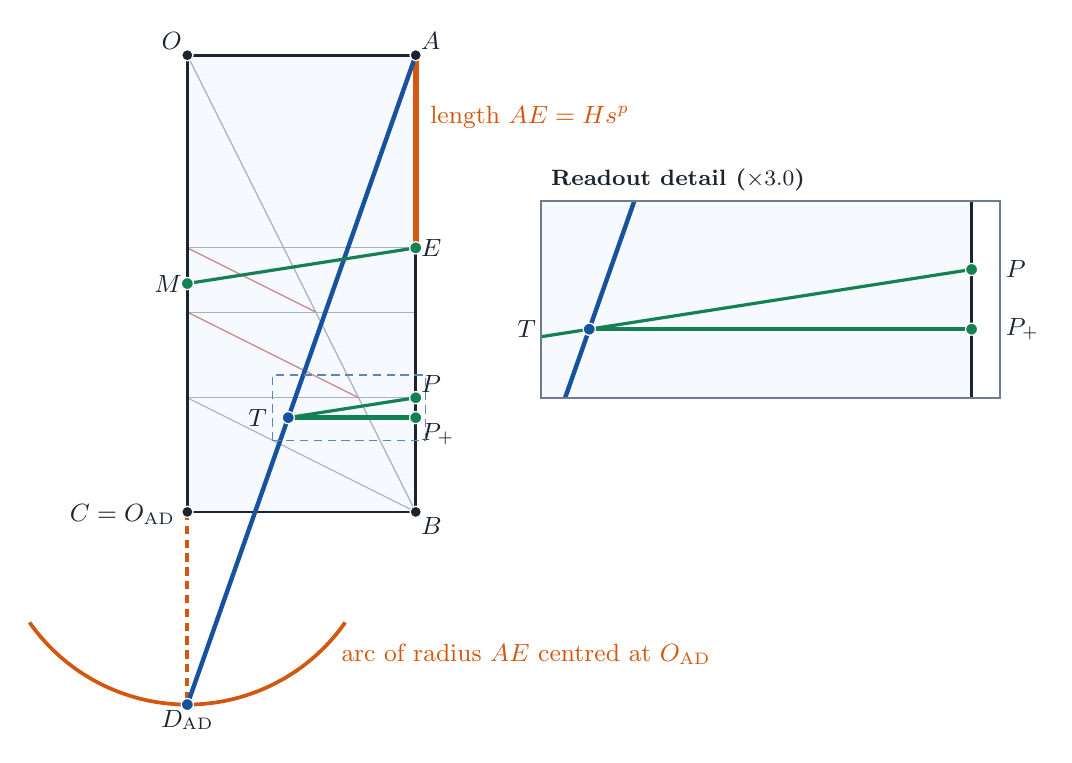
\begin{tikzpicture}[scale=1.45]
\fill[rectbg] (0.0000,0.0000) rectangle (2.0000,4.0000);
\draw[chain] (0.0000,4.0000)--(2.0000,0.0000);
\draw[chain] (0.0000,1.0000)--(2.0000,0.0000);
\draw[chain] (0,1.0000)--(2.0,1.0000);
\draw[chain] (0,1.7500)--(2.0,1.7500);
\draw[chain] (0,2.3125)--(2.0,2.3125);
\draw[chainpar] (1.5000,1.0000)--(0.0000,1.7500);
\draw[chainpar] (1.1250,1.7500)--(0.0000,2.3125);
\draw[rect] (0.0000,0.0000) rectangle (2.0000,4.0000);
\draw[accent] (0.0000,0.0000) ++(215:1.6875) arc (215:325:1.6875);
\draw[accent,densely dashed] (0.0000,0.0000)--(0.0000,-1.6875);
\draw[accent,line width=2.2pt] (2.0000,4.0000)--(2.0000,2.3125);
\draw[support] (2.0000,4.0000)--(0.0000,-1.6875);
\draw[transport] (0.0000,2.0000)--(2.0000,2.3125);
\draw[transport] (2.0000,1.0000)--(0.8837,0.8256);
\draw[transport,line width=1.65pt] (0.8837,0.8256)--(2.0000,0.8256);
\node[lab,above left] at (0.0000,4.0000) {$O$};
\node[lab,above right] at (2.0000,4.0000) {$A$};
\node[lab,anchor=east] at (-0.06,-0.02) {$C=O_{\mathrm{AD}}$};
\node[lab,below right] at (2.0000,0.0000) {$B$};
\node[pt] at (0.0000,4.0000) {};
\node[pt] at (2.0000,4.0000) {};
\node[pt] at (0.0000,0.0000) {};
\node[pt] at (2.0000,0.0000) {};
\node[pttrans] at (0.0000,2.0000) {};
\node[pttrans] at (2.0000,2.3125) {};
\node[pttrans] at (2.0000,1.0000) {};
\node[ptsupp] at (0.8837,0.8256) {};
\node[pttrans] at (2.0000,0.8256) {};
\node[lab,left] at (0.0000,2.0000) {$M$};
\node[lab,right] at (2.0000,2.3125) {$E$};
\node[lab,above right] at (2.0000,1.0000) {$P$};
\node[lab,below right] at (2.0000,0.8256) {$P_+$};
\node[ptsupp] at (0.0000,-1.6875) {};
\node[lab,below] at (0.0000,-1.6875) {$D_{\mathrm{AD}}$};
\node[lab,acc,anchor=west] at (2.0800,3.4562) {length $AE=Hs^p$};
\node[lab,acc,anchor=west] at (1.3,-1.25) {arc of radius $AE$ centred at $O_{\mathrm{AD}}$};
\draw[aux,supp!70] (0.7437,0.6256) rectangle (2.0840,1.2000);
\node[lab,left] at (0.7437,0.8256) {$T$};
\begin{scope}[shift={(0.8688,-0.8767)},scale=3.0]
\begin{scope}
\clip (0.7437,0.6256) rectangle (2.0840,1.2000);
\fill[white] (0.7437,0.6256) rectangle (2.0840,1.2000);
\fill[rectfill] (0.7437,0.6256) rectangle (2.0,1.2000);
\draw[rect] (2.0,-0.3744)--(2.0,2.2000);
\draw[support] (2.0000,4.0000)--(0.0000,-1.6875);
\draw[transport] (2.0000,1.0000)--(-3.0000,0.2188);
\draw[transport,line width=1.65pt] (0.8837,0.8256)--(2.0000,0.8256);
\node[pttrans] at (2.0000,1.0000) {};
\node[ptsupp] at (0.8837,0.8256) {};
\node[pttrans] at (2.0000,0.8256) {};
\end{scope}
\draw[line width=0.65pt,slatec] (0.7437,0.6256) rectangle (2.0840,1.2000);
\node[lab,right] at (2.0840,1.0000) {$P$};
\node[lab,right] at (2.0840,0.8256) {$P_+$};
\node[lab,left] at (0.7437,0.8256) {$T$};
\node[font=\footnotesize\bfseries,text=ink,anchor=south west] at (0.7437,1.2000) {Readout detail ($\times3.0$)};
\end{scope}
\end{tikzpicture}%
}

\newcommand{\figProjective}{%
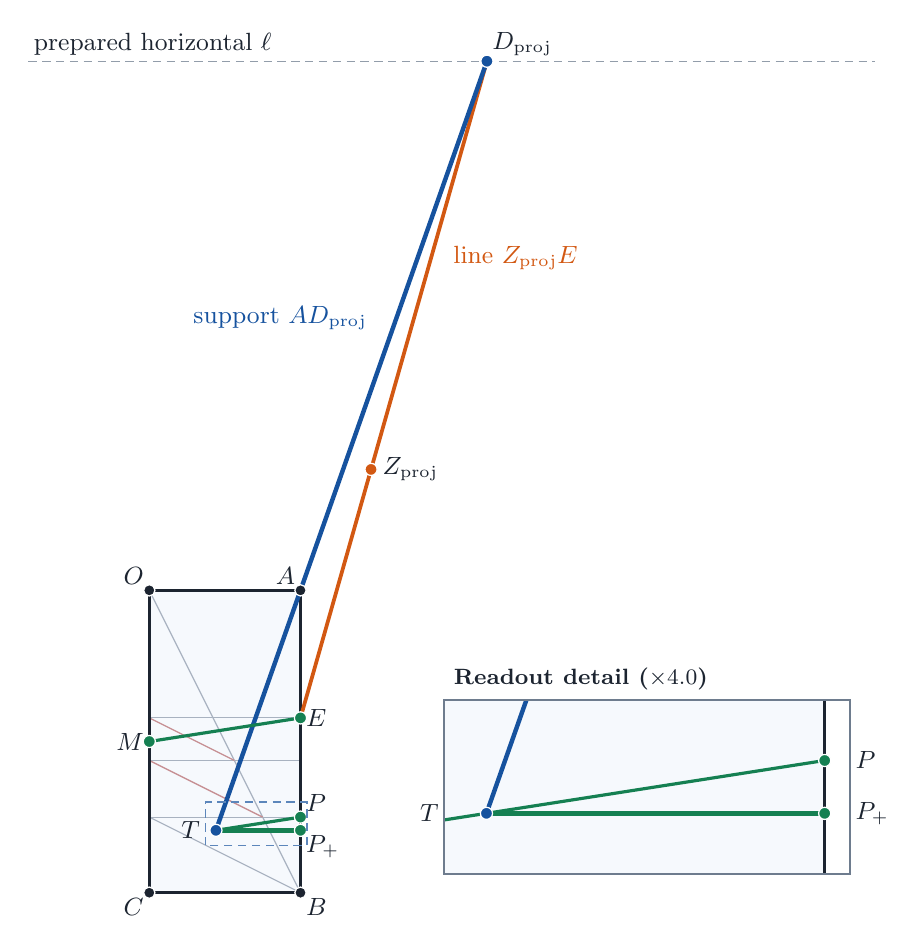
\begin{tikzpicture}[scale=0.96]
\draw[aux] (-1.6,11.0000)--(9.6,11.0000);
\node[lab,anchor=south west] at (-1.6,11.0000) {prepared horizontal $\ell$};
\fill[rectbg] (0.0000,0.0000) rectangle (2.0000,4.0000);
\draw[chain] (0.0000,4.0000)--(2.0000,0.0000);
\draw[chain] (0.0000,1.0000)--(2.0000,0.0000);
\draw[chain] (0,1.0000)--(2.0,1.0000);
\draw[chain] (0,1.7500)--(2.0,1.7500);
\draw[chain] (0,2.3125)--(2.0,2.3125);
\draw[chainpar] (1.5000,1.0000)--(0.0000,1.7500);
\draw[chainpar] (1.1250,1.7500)--(0.0000,2.3125);
\draw[rect] (0.0000,0.0000) rectangle (2.0000,4.0000);
\draw[accent] (2.0000,2.3125)--(4.4664,11.0000);
\draw[support] (0.8814,0.8252)--(4.4664,11.0000);
\draw[transport] (0.0000,2.0000)--(2.0000,2.3125);
\draw[transport] (2.0000,1.0000)--(0.8814,0.8252);
\draw[transport,line width=1.65pt] (0.8814,0.8252)--(2.0000,0.8252);
\node[lab,above left] at (0.0000,4.0000) {$O$};
\node[lab,above left] at (2.0000,4.0000) {$A$};
\node[lab,below left] at (0.0000,0.0000) {$C$};
\node[lab,below right] at (2.0000,0.0000) {$B$};
\node[pt] at (0.0000,4.0000) {};
\node[pt] at (2.0000,4.0000) {};
\node[pt] at (0.0000,0.0000) {};
\node[pt] at (2.0000,0.0000) {};
\node[pttrans] at (0.0000,2.0000) {};
\node[pttrans] at (2.0000,2.3125) {};
\node[pttrans] at (2.0000,1.0000) {};
\node[ptsupp] at (0.8814,0.8252) {};
\node[pttrans] at (2.0000,0.8252) {};
\node[lab,left] at (0.0000,2.0000) {$M$};
\node[lab,right] at (2.0000,2.3125) {$E$};
\node[lab,above right] at (2.0000,1.0000) {$P$};
\node[lab,below right] at (2.0000,0.8252) {$P_+$};
\node[ptacc] at (2.9333,5.6000) {};
\node[ptsupp] at (4.4664,11.0000) {};
\node[lab,right] at (3.0133,5.6000) {$Z_{\mathrm{proj}}$};
\node[lab,above right] at (4.4664,11.0000) {$D_{\mathrm{proj}}$};
\node[lab,acc,anchor=west] at (3.95,8.4) {line $Z_{\mathrm{proj}}E$};
\node[lab,supp,anchor=east] at (2.95,7.6) {support $AD_{\mathrm{proj}}$};
\draw[aux,supp!70] (0.7414,0.6252) rectangle (2.0840,1.2000);
\node[lab,left] at (0.7414,0.8252) {$T$};
\begin{scope}[shift={(0.9345,-2.2509)},scale=4.0]
\begin{scope}
\clip (0.7414,0.6252) rectangle (2.0840,1.2000);
\fill[white] (0.7414,0.6252) rectangle (2.0840,1.2000);
\fill[rectfill] (0.7414,0.6252) rectangle (2.0,1.2000);
\draw[rect] (2.0,-0.3748)--(2.0,2.2000);
\draw[support] (0.8814,0.8252)--(4.4664,11.0000);
\draw[transport] (2.0000,1.0000)--(-3.0000,0.2188);
\draw[transport,line width=1.65pt] (0.8814,0.8252)--(2.0000,0.8252);
\node[pttrans] at (2.0000,1.0000) {};
\node[ptsupp] at (0.8814,0.8252) {};
\node[pttrans] at (2.0000,0.8252) {};
\end{scope}
\draw[line width=0.65pt,slatec] (0.7414,0.6252) rectangle (2.0840,1.2000);
\node[lab,right] at (2.0840,1.0000) {$P$};
\node[lab,right] at (2.0840,0.8252) {$P_+$};
\node[lab,left] at (0.7414,0.8252) {$T$};
\node[font=\footnotesize\bfseries,text=ink,anchor=south west] at (0.7414,1.2000) {Readout detail ($\times4.0$)};
\end{scope}
\end{tikzpicture}%
}

\newcommand{\figMB}{%
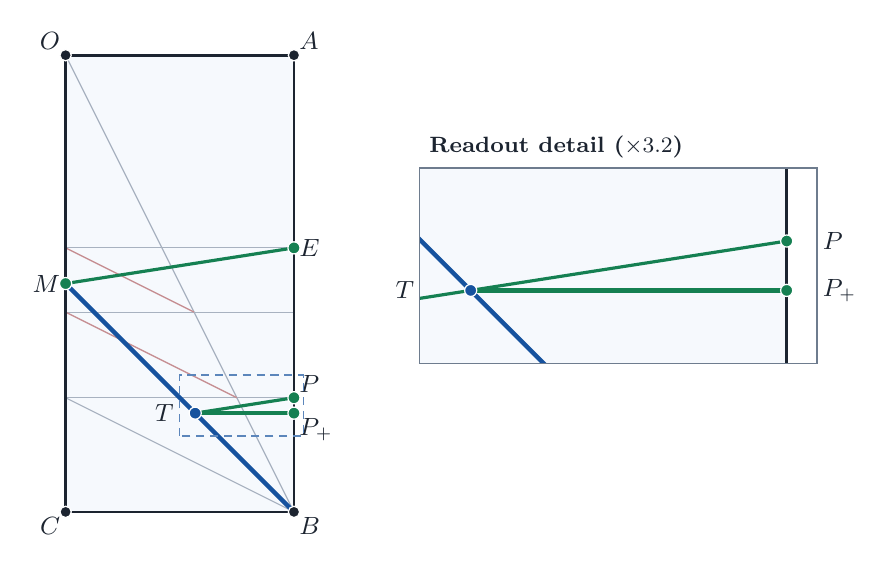
\begin{tikzpicture}[scale=1.45]
\fill[rectbg] (0.0000,0.0000) rectangle (2.0000,4.0000);
\draw[chain] (0.0000,4.0000)--(2.0000,0.0000);
\draw[chain] (0.0000,1.0000)--(2.0000,0.0000);
\draw[chain] (0,1.0000)--(2.0,1.0000);
\draw[chain] (0,1.7500)--(2.0,1.7500);
\draw[chain] (0,2.3125)--(2.0,2.3125);
\draw[chainpar] (1.5000,1.0000)--(0.0000,1.7500);
\draw[chainpar] (1.1250,1.7500)--(0.0000,2.3125);
\draw[rect] (0.0000,0.0000) rectangle (2.0000,4.0000);
\draw[support] (0.0000,2.0000)--(2.0000,0.0000);
\draw[transport] (0.0000,2.0000)--(2.0000,2.3125);
\draw[transport] (2.0000,1.0000)--(1.1351,0.8649);
\draw[transport,line width=1.65pt] (1.1351,0.8649)--(2.0000,0.8649);
\node[lab,above left] at (0.0000,4.0000) {$O$};
\node[lab,above right] at (2.0000,4.0000) {$A$};
\node[lab,below left] at (0.0000,0.0000) {$C$};
\node[lab,below right] at (2.0000,0.0000) {$B$};
\node[pt] at (0.0000,4.0000) {};
\node[pt] at (2.0000,4.0000) {};
\node[pt] at (0.0000,0.0000) {};
\node[pt] at (2.0000,0.0000) {};
\node[pttrans] at (0.0000,2.0000) {};
\node[pttrans] at (2.0000,2.3125) {};
\node[pttrans] at (2.0000,1.0000) {};
\node[ptsupp] at (1.1351,0.8649) {};
\node[pttrans] at (2.0000,0.8649) {};
\node[lab,left] at (0.0000,2.0000) {$M$};
\node[lab,right] at (2.0000,2.3125) {$E$};
\node[lab,above right] at (2.0000,1.0000) {$P$};
\node[lab,below right] at (2.0000,0.8649) {$P_+$};
\draw[aux,supp!70] (0.9951,0.6649) rectangle (2.0840,1.2000);
\node[lab,left] at (0.9951,0.8649) {$T$};
\begin{scope}[shift={(-0.0844,-0.8276)},scale=3.2]
\begin{scope}
\clip (0.9951,0.6649) rectangle (2.0840,1.2000);
\fill[white] (0.9951,0.6649) rectangle (2.0840,1.2000);
\fill[rectfill] (0.9951,0.6649) rectangle (2.0,1.2000);
\draw[rect] (2.0,-0.3351)--(2.0,2.2000);
\draw[support] (0.0000,2.0000)--(2.0000,0.0000);
\draw[transport] (2.0000,1.0000)--(-3.0000,0.2188);
\draw[transport,line width=1.65pt] (1.1351,0.8649)--(2.0000,0.8649);
\node[pttrans] at (2.0000,1.0000) {};
\node[ptsupp] at (1.1351,0.8649) {};
\node[pttrans] at (2.0000,0.8649) {};
\end{scope}
\draw[line width=0.65pt,slatec] (0.9951,0.6649) rectangle (2.0840,1.2000);
\node[lab,right] at (2.0840,1.0000) {$P$};
\node[lab,right] at (2.0840,0.8649) {$P_+$};
\node[lab,left] at (0.9951,0.8649) {$T$};
\node[font=\footnotesize\bfseries,text=ink,anchor=south west] at (0.9951,1.2000) {Readout detail ($\times3.2$)};
\end{scope}
\end{tikzpicture}%
}



\pagestyle{fancy}\fancyhf{}
\fancyhead[L]{\small\textcolor{slatec}{Geometric root calculators}}
\fancyhead[R]{\small\textcolor{slatec}{V31 / Research preprint}}
\fancyfoot[C]{\small\thepage}
\renewcommand{\headrulewidth}{0.3pt}
\setlength{\parindent}{0pt}\setlength{\parskip}{5.5pt plus 1pt}
\setlist{itemsep=2.5pt,topsep=3pt}

\theoremstyle{plain}
\newtheorem{theorem}{Theorem}[section]
\newtheorem{proposition}[theorem]{Proposition}
\newtheorem{lemma}[theorem]{Lemma}
\newtheorem{corollary}[theorem]{Corollary}
\theoremstyle{remark}
\newtheorem{remark}[theorem]{Remark}
\numberwithin{equation}{section}

% ---- clean callout box for intuition and roadmap (pure TikZ, no extra packages) ----
\newcommand{\keyidea}[2]{%
  \par\vspace{3pt}\noindent
  \begin{tikzpicture}
    \node[anchor=north west,inner xsep=10pt,inner ysep=7pt,text width=\dimexpr\linewidth-24pt\relax,
          fill=rectfill,rounded corners=2pt,draw=slatec!25,line width=0.4pt] (box)
          {\small\textcolor{supp}{\textbf{#1.}}\enspace #2};
    \fill[supp] (box.north west) rectangle ([xshift=2.6pt]box.south west);
  \end{tikzpicture}\par\vspace{3pt}%
}

% ---- notation macros ---------------------------------------------------
\newcommand{\jn}{\mathsf{j}}          % one join
\newcommand{\pl}{\mathsf{p}}          % one constructed parallel (= 2j + 3c)
\newcommand{\ar}{\mathsf{c}}          % one compass arc
\newcommand{\Om}{\Omega}              % projection centres on the top line
\newcommand{\cE}{\mathcal{E}}\newcommand{\cC}{\mathcal{C}}\newcommand{\cD}{\mathcal{D}}
\newcommand{\cU}{\mathcal{U}}\newcommand{\cV}{\mathcal{V}}\newcommand{\cR}{\mathcal{R}}
\newcommand{\cJ}{\mathcal{J}}\newcommand{\cA}{\mathcal{A}}\newcommand{\cB}{\mathcal{B}}
\newcommand{\cK}{\mathcal{K}}\newcommand{\cM}{\mathcal{M}}\newcommand{\cP}{\mathcal{P}}
\newcommand{\Tm}{\mathrm{T}}
\newcommand{\eps}{\varepsilon}
\DeclareMathOperator{\disc}{disc}

\begin{document}

\noindent\textcolor{supp}{\rule{\linewidth}{1.6pt}}
\vspace{4pt}

{\small\scshape\textcolor{slatec}{Constructive geometry \,/\, root iterations \,/\, global convergence}}

\vspace{5pt}
{\LARGE\bfseries\textcolor{ink}{Geometric Root Calculators}\par}
\vspace{3pt}
{\large\raggedright\textcolor{ink!85}{Radical supports of orders five and nine and real-degree enclosures in the Pandrosion rectangle}\par}
\vspace{8pt}
Ivan Besevic\footnote{Computational assistance: the AI systems ChatGPT (OpenAI), Claude (Anthropic) and Gemini (Google) were used for derivations, proof development,
figures and manuscript preparation. The author is responsible for the claims and their attribution.
Section~\ref{sec:evidence} states, claim by claim, which results are formal proofs, written proofs,
computer-algebra identities or numerical checks.}
\quad$\cdot$\quad Independent research\\
Version 31 (revision of V30) \quad$\cdot$\quad 23 November 2026\\
\url{https://github.com/ivan-fr/pandrosion}

\vspace{6pt}
\begin{quote}\small
\textbf{Abstract.}
We study ruler-and-compass iterations for the positive root $X^{1/p}$ that share one rectangle, one
power stage and one readout, and differ only in a \emph{support line}. Every support approximates the
same target function $\kappa_*(t)=(t-1)/(t^{1/p}-1)$ of the residual $t$, and the contact order of the
approximation fixes the order of the iteration. Besides the classical supports of orders one to four we
treat two radical supports. A decentered arc gives a globally monotone fifth-order iteration. A
combination of the arithmetic mean, the geometric mean and one conic mean of $1$ and $t$, drawn with three
arcs, has local order \emph{exactly nine for every real $p>2$}, with error constant $23/20736$ for cube
roots, and converges monotonically from every positive start. For integer $p\ge 3$ one step costs at
most $10p+9$ elementary traces for the decentered arc and $10p+11$ for the three-mean support; measured
by the efficiency index, and under the stated counting conventions, the three-mean support is preferable
for every $p\ge3$. We then separate what is a finite construction from what is only a scalar statement:
the fast iterations are finite constructions for rational degrees, whereas for irrational $p$ a single
step is not. For arbitrary real $p\neq 0$ a power-free subdivision with one final Pad\'e readout encloses
the root with relative width at most $z^5/256$ in at most $15n+63$ traces after $n$ subdivisions (for
$X>1$, $p\ge 1$). Global convergence and the local orders with their constants, for both radical
supports and every real $p>2$, are checked in Lean, as are the approximation and efficiency statements;
the drawing inventories are written protocols.
\end{quote}

% =========================================================================
\section{Introduction}

How fast can a ruler-and-compass iteration compute $\sqrt[3]{2}$---or any positive $p$th root $X^{1/p}$?
Unlike a numerical algorithm written in floating-point arithmetic, a geometric iteration must realize every
operation by intersections, parallels and compass transfers.

The Pandrosion rectangle provides a single geometric chassis for all $p$th roots (Figure~\ref{fig:anatomy}).
Starting from a current reciprocal estimate $s$ on the right rail, a chain of similar triangles produces
its $p$th power $s^{p}$ (panel~1); a single line through a prepared point $M$ transports the residual
$t=Xs^{p}$ across the rectangle, and a horizontal returns the next estimate $s_+$ on the same rail
(panel~2). \emph{Only one element changes from one method to another:} the \emph{support}, a line through
the upper-right corner $A$ whose slope encodes a correction factor. Replacing a fixed line by one
decentered compass arc lifts the convergence order from two to five; replacing it by three arcs encoding
three classical means lifts the order to nine---turning a $5.5\%$ initial error for $\sqrt[3]{2}$ into
fourteen correct digits in a single geometric step (panel~3).

\begin{figure}[htbp]
\centering\figAnatomy
\caption{Anatomy of the Pandrosion rectangle for $p=3$, $X=2$, $s_0=3/4$ (initial relative error $5.5\%$).
\textbf{(1)~Power stage:} parallels to $L_1B$ through the diagonal points $B_j$ multiply by $s$ at each step,
producing $E=R(s^{3})$.
\textbf{(2)~Transport and readout:} the line $ME$ encodes the residual $t=Xs^{p}$; its parallel through $P$
meets the support through $A$ at $T$, and the horizontal reads $P_+=R(s_+)$.
\textbf{(3)~One line changes the order:} exact digits of accuracy $-\log_{10}|s_+/\alpha-1|$ after a
\emph{single} step from $s_0=3/4$, for all six supports studied in this paper.}\label{fig:anatomy}
\end{figure}

\paragraph{Main results.}
\begin{enumerate}[label=\arabic*.]
\item \textbf{One target function} (Section~\ref{sec:coords}). Every support through $A$ approximates the
  same target slope $\kappa_*(t)=(t-1)/(t^{1/p}-1)$; contact of order $\omega$ at $t=1$ produces an
  iteration of order $\omega+1$ with an explicit error constant (Lemma~\ref{lem:contact}). Newton, Halley
  and the $[1/1]$ Pad\'e support are the classical cases $\omega=1,2,3$.
\item \textbf{Decentered arc---order five at the cost of order three} (Section~\ref{sec:arc}). Shifting the
  compass centre of Halley's construction off the target vertical gives $\omega=4$: a globally monotone
  fifth-order iteration for every real $p>2$, using the same mobile operations as Halley (one arc and one
  join; Theorem~\ref{thm:arc}).
\item \textbf{Three means---order nine in three arcs} (Section~\ref{sec:mean}). A linear combination of the
  arithmetic mean, the geometric mean and one conic mean of $1$ and $t$ achieves $\omega=8$. It is drawn
  with three arcs and one join, has local order \emph{exactly nine} for every real $p>2$ with closed-form
  constant $c_M(p)$ ($c_M(3)=23/20736$), and converges monotonically from every positive start
  (Theorem~\ref{thm:mean}).
\item \textbf{Finite-step degrees and direct real-degree enclosures} (Sections~\ref{sec:degrees}
  and~\ref{sec:enclosure}). The fast iterations have finite ruler-and-compass steps precisely for integer
  and rational degrees (Table~\ref{tab:degrees}); for arbitrary real $p\neq0$ (including irrational $p$), a
  power-free geometric subdivision with one final $[2/2]$ Pad\'e readout certifies $X^{1/p}$ to relative
  width at most $z^{5}/256$ in at most $15n+63$ traces after $n$ subdivisions
  (Propositions~\ref{prop:enclosure} and~\ref{prop:allp}).
\item \textbf{Geometric work and efficiency} (Section~\ref{sec:work}). Under the stated trace-counting
  conventions, one step costs at most $10p+9$ traces for the decentered arc and $10p+11$ for the three-mean
  support (Proposition~\ref{prop:mean-inventory}); measured by Ostrowski's efficiency index, the three-mean
  support leads all six rectangle supports at every integer degree $p\ge3$ (Proposition~\ref{prop:index}).
\end{enumerate}

\begin{table}[htbp]
\centering\small
\caption{Which calculator applies to which degree. ``Finite step'' means that one iteration step is a
finite ruler-and-compass construction from the current state.}\label{tab:degrees}
\begin{tabularx}{\linewidth}{@{}lXX@{}}
\toprule
Degree $p$ & Fast rectangle iterations (orders 2--9) & Direct subdivision (Section~\ref{sec:enclosure})\\
\midrule
Integer $p\ge 3$ & Finite step; $10p+9$ or $10p+11$ traces & Yes\\
Rational $p=\mu/\nu$ & Finite step, as degree $\mu$ applied to $X^{\nu}$ (Proposition~\ref{prop:rational}) & Yes\\
Irrational $p$ & Step not finite: $u^{p}$ is itself a real power. Available only through a rational
approximation of $p$ (Proposition~\ref{prop:irrational}) & Yes; this is the recommended route\\
\bottomrule
\end{tabularx}
\end{table}

\paragraph{What ``construct'' means here.}
As in Pandrosion's recursive geometry, nothing in this paper constructs $X^{1/p}$ exactly in finitely
many operations; $\sqrt[3]{2}$ is not constructible. A calculator is a rule whose every step is a finite
construction and whose successive outputs converge to the root, with a stated rate or a stated
enclosure. The distinction that matters is therefore not exact versus approximate, but whether
\emph{each step} is finite. Scalar convergence theorems are stated for real $p$; drawing inventories are
stated only where a step is a finite construction.

\keyidea{Guide to the paper}{%
\textbf{Section~\ref{sec:coords}} sets up the rectangle, line arithmetic and the common target
$\kappa_*(t)$.
\textbf{Sections~\ref{sec:arc} and~\ref{sec:mean}} develop the two radical supports (orders $5$ and $9$);
heavy polynomial certificate coefficients are placed in Appendix~\ref{app:certs} to keep the main text
readable.
\textbf{Sections~\ref{sec:degrees}--\ref{sec:enclosure}} classify finite-step degrees, compare trace costs
and efficiency indices, and build the direct subdivision calculator for arbitrary real degrees.
\textbf{Sections~\ref{sec:attribution}--\ref{sec:conclusion}} cover attribution, Lean/CAS verification,
revision history, scope limits and open questions; classical supports and equivalence remarks appear in
Appendices~\ref{app:classical}--\ref{app:equiv}.}

% =========================================================================
\section{Coordinates, arithmetic and the common target $\kappa_*$}\label{sec:coords}

\subsection{States and notation}

For $X>0$ and $p\neq 0$ let $r=X^{1/p}$ be the root and $\alpha=1/r$ its reciprocal. The rectangle
carries a \emph{reciprocal state} $s>0$ approaching $\alpha$; the \emph{direct state} is $u=1/s$. The
\emph{residual} is
\[ t=Xs^{p}=X/u^{p}, \qquad t=1 \iff s=\alpha . \]
The logarithmic error is $e=\log(s/\alpha)$, so that $t=e^{pe}$. An iteration is written
$s_+=s\,\Phi(t)$. Table~\ref{tab:notation} groups the main symbols by role.

\begin{table}[htbp]
\centering\small
\caption{Notation, grouped by role.}\label{tab:notation}
\begin{tabularx}{\linewidth}{@{}lX@{}}
\toprule
\multicolumn{2}{@{}l}{\textbf{Problem, states and errors}}\\
$X,\ p,\ r,\ \alpha$ & input, degree, root $X^{1/p}$, reciprocal root $X^{-1/p}$\\
$s,\ u,\ t,\ e$ & reciprocal state, direct state $1/s$, residual $Xs^p$, log error $\log(s/\alpha)$\\
$h,\ \xi,\ x$ & $h=1/p$;\ \ $\xi=t-1$;\ \ $x=\log t=pe$\\
$\mu,\ \nu$ & coprime numerator and denominator of a rational degree $p=\mu/\nu$\\
\midrule
\multicolumn{2}{@{}l}{\textbf{Rectangle and line arithmetic (Section~\ref{sec:rect})}}\\
$W,H$; $A,B,C,O$ & rectangle width and height; its corners\\
$R(q),\ L(q),\ \Om_f$ & right-rail point, left-rail point, projection centre on the top line\\
$M,\ E,\ P,\ T$ & prepared point $L(X^{-1})$, power endpoint $R(s^{p})$, state $R(s)$, support intersection\\
\midrule
\multicolumn{2}{@{}l}{\textbf{Supports and trace counts (Sections~\ref{sec:coords}--\ref{sec:work})}}\\
$\kappa,\ \kappa_*,\ \omega$ & normalized support slope; exact slope $(t-1)/(t^{h}-1)$; contact order at $t=1$\\
$q_5,\ q_M$ & normalized slopes $(\kappa-1)/(p-1)$ of the decentered and three-mean supports\\
$m,g,n,d$;\ $\tau,\lambda_X$ & (Section~\ref{sec:mean}) coefficients of $q_M$;\ \ $\tau=\sqrt t$,\ \ $\lambda_X=H/X$\\
$\jn,\ \pl,\ \ar$ & one join, one constructed parallel ($=2\jn+3\ar$), one compass arc\\
\midrule
\multicolumn{2}{@{}l}{\textbf{Direct subdivision (Section~\ref{sec:enclosure})}}\\
$a,\ b,\ m_{\mathrm{g}}$ & moving positive rail endpoints and their mean proportional $\sqrt{ab}$\\
$\lambda,\ z$ & moving exponent weight $\lambda\in[0,1]$ and rail gap $z=b/a-1$\\
\bottomrule
\end{tabularx}
\end{table}

\subsection{Rectangle and line arithmetic}\label{sec:rect}

In the rectangle $C=(0,0)$, $B=(W,0)$, $O=(0,H)$, $A=(W,H)$, with $W,H>0$, define
\begin{equation}\label{eq:rails}
R(q)=(W,H(1-q)),\qquad L(q)=(0,H(1-q)),\qquad \Om_f=\Bigl(\frac{Wf}{f-1},\,H\Bigr)\quad(f\neq 1).
\end{equation}
Line incidences perform multiplication and division:
\begin{equation}\label{eq:incid}
\Om_fR(q)\cap OC=L(fq),\qquad \Om_fL(b)\cap AB=R(b/f).
\end{equation}
Substituting the coordinates into the line equations proves both identities. Unit factors and zero
values reuse existing points instead of a centre at infinity.

\paragraph{Triangle power stage.}
As shown in Figure~\ref{fig:anatomy}(1), let $B_j=(Ws^{j},H(1-s^{j}))\in OB$ and $L_j=L(s^{j})$.
Horizontals transfer between these points and the rails. The parallel to $L_1B$ through $B_j$ meets the
left rail at $L_{j+1}$, since its ordinate there is $H(1-s^{j})+H(1-s)s^{j}=H(1-s^{j+1})$. For integer
$p$, repetition gives $E=R(s^{p})$ with $2p-1$ parallels and the join $L_1B$.

\paragraph{Products.}
For positive rail values $a,b$ with $b\neq 1$, draw $V=CR(b)\cap OA=\Om_{1/b}$ and project $R(a)$
successively through $\Om_{1/2}$, $V$, $\Om_{1/2}$, $\Om_{1/4}$. By~\eqref{eq:incid} the successive
values are $L(a/2)$, $R(ab/2)$, $L(ab/4)$, $R(ab)$: a general product costs five joins. Division is
symmetric: project $R(a)$ through $V$ to $L(a/b)$ and return through $\Om_{1/2},\Om_{1/4},\Om_{1/2}$,
with values $R(2a/b)$, $L(a/(2b))$, $R(a/b)$; again five joins. Multiplication by a \emph{prepared}
constant $d>0$ uses the two centres $\Om_{d/[2(1+d)]}$ and $\Om_{1/[2(1+d)]}$ and costs two joins.

\subsection{The common support equation and its target}

Prepare $M=(0,H(1-X^{-1}))$. With $P=R(s)$ and $E=R(s^{p})$, the line $ME$ has slope
$\sigma=H(1-t)/(WX)$. Let a \emph{support} be a line through $A$ of slope $H\kappa/(WX)$. As illustrated in
Figure~\ref{fig:anatomy}(2), the parallel to $ME$ through $P$ meets the support at $T$, and the horizontal
through $T$ meets the right rail at $P_+=R(s_+)$ with
\begin{equation}\label{eq:support}
s_+=s\,\frac{\kappa}{\kappa-1+t}.
\end{equation}
Indeed the two lines are $y-H=\tfrac{H\kappa}{WX}(x-W)$ and $y-H(1-s)=\sigma(x-W)$; eliminating $x$
gives $H-y=Hs\kappa/(\kappa-1+t)$. The update is exact, $s_+=\alpha$, precisely when
$\kappa/(\kappa-1+t)=t^{-h}$, that is when
\begin{equation}\label{eq:kstar}
\kappa=\kappa_*(t):=\frac{t-1}{t^{h}-1}\qquad(\kappa_*(1)=p).
\end{equation}
The function $\kappa_*$ is not constructible from $t$; every support in this paper is a constructible
approximation of it (Figure~\ref{fig:target}).

\begin{lemma}[Contact lemma; limit form formalized in Lean]\label{lem:contact}
Let $\kappa(t)$ be analytic and positive near $t=1$ with
$\kappa(t)-\kappa_*(t)=c\,\xi^{\omega}+O(\xi^{\omega+1})$, $\xi=t-1$, $\omega\ge1$. Then the iteration
\eqref{eq:support} satisfies
\[ e_+=c\,p^{\,\omega-1}e^{\,\omega+1}+O(e^{\,\omega+2}). \]
\end{lemma}
\begin{proof}
From \eqref{eq:support}, $e_+=e+\log\kappa-\log(\kappa-1+t)$, and this vanishes for
$\kappa=\kappa_*$. Since $\partial_\kappa[\log\kappa-\log(\kappa-1+t)]=(t-1)/[\kappa(\kappa-1+t)]$,
which equals $\xi/p^{2}+O(\xi^{2})$ near $\kappa=p$, we get
$e_+=c\,\xi^{\omega+1}/p^{2}+O(\xi^{\omega+2})$. Finally $\xi=e^{pe}-1=pe+O(e^{2})$.
\end{proof}

\begin{figure}[htbp]
\centering\figTarget
\caption{Every support approximates the same target function $\kappa_*(t)=(t-1)/(t^{1/p}-1)$ (shown here
for $p=3$).
\textbf{(a)}~The normalized slopes $\kappa(t)$ across $t\in[0.15,2.4]$: AK is the constant value at $t=1$,
AD is the tangent line, projective AD is the $[1/1]$ Pad\'e hyperbola, the decentered arc hugs $\kappa_*$
closely, and the three-mean support is visually indistinguishable from $\kappa_*$.
\textbf{(b)}~Log--log plot of the slope error $|\kappa(t)-\kappa_*(t)|$ against $\xi=t-1$: the five
supports descend with exact slopes $\omega=1,2,3,4,8$, which by Lemma~\ref{lem:contact} determine their
iteration orders $2,3,4,5,9$.}\label{fig:target}
\end{figure}

\begin{table}[htbp]
\centering\small
\caption{The supports as approximations of $\kappa_*$. Leading constants are for the reciprocal-state
log error $e$; for odd orders they are unchanged in the direct state.}\label{tab:supports}
\begin{tabular}{@{}llccl@{}}
\toprule
Support & $\kappa(t)$ & contact $\omega$ & order & leading constant of $e_+$\\
\midrule
AK (Newton) & $p$ & 1 & 2 & $-(p-1)/2$\\[2pt]
AD (Halley) & $\tfrac12[p+1+(p-1)t]$ & 2 & 3 & $(p^{2}-1)/12$\\[2pt]
Projective AD & $\dfrac{2p[(2p-1)t+p+1]}{(p+1)t+5p-1}$ & 3 & 4 & $-(p^{2}-1)(2p-1)/72$\\[6pt]
Decentered AD & $1+(p-1)q_5(t)$ & 4 & 5 & $(p-2)(p^{2}-1)(3p+1)/1440$\\[2pt]
Three means & $1+(p-1)q_M(t)$ & 8 & 9 & $c_M(p)$, Theorem~\ref{thm:mean}\\
\bottomrule
\end{tabular}
\end{table}

AK is the value of $\kappa_*$ at $t=1$, AD its first-order Taylor polynomial and projective AD its
$[1/1]$ Pad\'e approximant; these three are classical (Newton under inversion, Halley, and a Pad\'e
correction) and are documented with full drawings in Appendix~\ref{app:classical}. The linear MB
construction uses the support $MB$, which does not pass through $A$, and is kept as a baseline in
Appendix~\ref{app:mb}.

\subsection{Work convention}\label{sec:convention}

A \emph{trace} is one join or one compass arc. A constructed parallel expands to $\pl=2\jn+3\ar$, five
traces. Intersections of drawn objects are free. \emph{Fixed preparation}, meaning every object that
depends only on $p,X,W,H$ and not on the current state, is not charged, nor are decisions (comparisons
of two constructed lengths) or the single final inversion that converts $s$ into $u=1/s$. Section
\ref{sec:enclosure} charges its input and output inversions explicitly. All counts are upper bounds for
the specified protocols; a trace count is neither a time nor an energy.

The name Pandrosion refers to the addressee of Book~III of Pappus' \emph{Collection}~\cite{pappus}. Our
rectangle follows a modern reconstruction~\cite{launay}; the accelerated supports are modern and are not
attributed to the ancient text.

% =========================================================================
\section{A decentered arc with global fifth-order convergence}\label{sec:arc}

\keyidea{Geometric idea}{%
Halley's construction (Appendix~\ref{app:classical}) transfers the length $AE=Hs^{p}$ straight down from a
prepared centre $O_{\mathrm{AD}}$ onto the vertical through $O_{\mathrm{AD}}$, producing a linear function
of $t$ and order $3$. Moving the prepared compass centre \emph{sideways} by a fixed offset $\delta$ forces
the arc to intersect the vertical by Pythagoras, replacing a linear transfer by $\sqrt{R^{2}-\delta^{2}}$.
With the right preparation constants, that single square root cancels two additional Taylor terms of
$\kappa_*$---raising the order from three to five at zero extra mobile work.}

\subsection{Formula and construction}

For real $p>2$ put
\begin{equation}\label{eq:arc}
S(t)=(p-2)(t^{2}+1)+(10p+4)t,\qquad q_5(t)=\sqrt{\frac{S(t)}{12p}},\qquad
\Tm_{\mathrm{arc}}(s)=s\,\frac{1+(p-1)q_5(t)}{t+(p-1)q_5(t)},
\end{equation}
that is, the support $\kappa=1+(p-1)q_5(t)$ in~\eqref{eq:support}. The radicand is positive for $t>0$.

For integer $p\ge3$ the radical is produced by one arc. Put
\[ \eta=(p-1)\sqrt{\frac{p-2}{12p}},\qquad \zeta=\frac{5p+2}{p-2}>1,\qquad d_0=\frac{W}{\eta},\qquad
\delta=\frac{H}{X}\sqrt{\zeta^{2}-1}, \]
and prepare
\[ G_0=\Bigl(W,\;H+\frac{H\zeta}{X}\Bigr),\qquad
O_{\mathrm{arc}}=\Bigl(W-d_0+\delta,\;H-\frac{H}{X\eta}\Bigr),\qquad\text{the vertical } x=W-d_0 . \]
Draw the arc centred at $O_{\mathrm{arc}}$ with radius $EG_0=(H/X)(t+\zeta)$ and take its lower
intersection $D_{\mathrm{arc}}$ with the prepared vertical. Its distance below the centre is
\[ \sqrt{EG_0^{2}-\delta^{2}}=\frac{H}{X}\sqrt{t^{2}+2\zeta t+1}, \]
so the slope of $AD_{\mathrm{arc}}$ is $\tfrac{H}{WX}\bigl[1+\eta\sqrt{t^{2}+2\zeta t+1}\bigr]
=\tfrac{H}{WX}\bigl[1+(p-1)q_5(t)\bigr]$, because $(p-2)\cdot2\zeta=10p+4$. All preparation parameters
use rational operations and square roots of positive quantities. Centered AD and decentered AD use the
same mobile operations, one arc and one join; only the fixed preparation differs. This is the precise
sense in which order five is obtained at the mobile cost of order three.

\begin{figure}[htbp]
\centering\figDecentered
\caption{The decentered-arc device for $p=7$, $X=W=2$, $H=4$, $s=3/4$, drawn from the exact coordinates.
\textbf{(a)~Circle and Pythagoras geometry:} the compass opening $EG_0$ (thick orange segment) is carried
to the prepared centre $O_{\mathrm{arc}}$; the circle meets the prepared vertical at $D_{\mathrm{arc}}$,
and the shaded right triangle with horizontal leg $\delta$ explains why the vertical leg is a square root.
\textbf{(b)~Support and readout:} the rectangle enlarged, showing the triangle chain (grey), transport
lines (green), support $AD_{\mathrm{arc}}$ (blue) and readout $P_+$. Each panel has equal axis
scales.}\label{fig:arc}
\end{figure}

\subsection{Global monotone convergence}

\begin{theorem}[Formalized in Lean]\label{thm:arc}
For real $p>2$, $X>0$ and every $s_0>0$, the iteration $s_{n+1}=\Tm_{\mathrm{arc}}(s_n)$ converges to
$\alpha$ monotonically without crossing it, and
\begin{equation}\label{eq:arc-order}
e_+=\frac{(p-2)(p^{2}-1)(3p+1)}{1440}\,e^{5}+O(e^{7}).
\end{equation}
\end{theorem}

\begin{proof}
Write $g=(p-1)q_5$. Since $S(1/t)=S(t)/t^{2}$ we have $q_5(1/t)=q_5(t)/t$, hence
$\Phi(1/t)=1/\Phi(t)$ for $\Phi=(1+g)/(t+g)$: the log-error map $e\mapsto e_+$ is odd. Put
\[ \Lambda(t)=\frac{\log t}{p}+\log(1+g(t))-\log(t+g(t)), \]
so that $e_+=\Lambda(t)$, and define the polynomials
\begin{align*}
N_1(t)&=(p-1)(t^{2}+1)+(10p+2)t,\\
N_2(t)&=(t+1)\bigl(6pt-(t-1)^{2}\bigr),\\
N_3(t)&=(p^{2}-5p-2)(t-1)^{2}+12p(3p+1)t .
\end{align*}
Differentiation and factorization give the two identities
\begin{align}
\frac{d\Lambda}{d\log t}&=\frac{(p-2)(p-1)^{2}\,\bigl(q_5N_1-N_2\bigr)}{12p^{2}\,g(1+g)(t+g)},\label{eq:arc-der}\\
q_5^{2}N_1^{2}-N_2^{2}&=\frac{p+1}{12p}\,(t-1)^{4}\,N_3 .\label{eq:arc-id}
\end{align}
Here $N_1>0$. If $N_2\le0$ then $q_5N_1-N_2>0$. Otherwise $(t-1)^{2}<6pt$, and $N_3>0$: directly when
$p^{2}-5p-2\ge0$, and otherwise from the rearrangement
\[ N_3=6p^{2}(p+1)t+(p^{2}-5p-2)\bigl((t-1)^{2}-6pt\bigr), \]
whose two terms are positive. Then \eqref{eq:arc-id} gives $q_5N_1>N_2$ for $t\neq1$. Hence $\Lambda$
is strictly increasing with $\Lambda(1)=0$: the new log error has the sign of the old one. Meanwhile
$\Phi(t)-1=(1-t)/(t+g)$ moves the state toward $\alpha$. The orbit is monotone and bounded between
$s_0$ and $\alpha$; its positive limit is a fixed point by continuity, and $\Phi(t)=1$ forces $t=1$.

Near $t=1$, rationalize $q_5N_1-N_2$ with \eqref{eq:arc-id}. At $t=1$ one has $q_5=1$, $g=p-1$,
$N_1=N_2=12p$ and $N_3=12p(3p+1)$, so
\[ \lim_{t\to1}\frac{d\Lambda/d\log t}{(t-1)^{4}}=\frac{(p-2)(p^{2}-1)(3p+1)}{288\,p^{5}} . \]
Substituting $t=e^{pe}$ and integrating yields the coefficient in \eqref{eq:arc-order}; oddness removes
the $e^{6}$ term.
\end{proof}

At $p=3$ the constant is $1/18$. At $p=2$ the scalar formula is an exact square-root correction, but
the displayed preparation is singular and is replaced by a single mean proportional.

% =========================================================================
\section{A three-mean support of order nine}\label{sec:mean}

\keyidea{Geometric idea}{%
The decentered arc matches one coefficient of the exact target $q_*/\sqrt{t}$ using one radical and one
arc. Combining three members of the same family---the arithmetic mean $\mathrm A=(1+t)/2$, the geometric
mean $\mathrm G=\sqrt{t}$ and one conic mean $\mathrm C_d=\sqrt{t+d(t-1)^{2}}$---gives three free
parameters and matches \emph{three} coefficients, jumping straight to contact eight and order nine.
Geometrically, the transport line $ME$ delivers the residual to three prepared verticals for free, so the
entire support costs only \emph{three compass arcs and one join}---just two traces more than Halley or
the decentered arc. Analytically, changing variable to $\tau=\sqrt{t}$ leaves only one square root, so
global convergence is proved by a single rationalization.}

\subsection{Formula}

The exact support is $\kappa_*=1+(p-1)q_*$ with
\[ q_*(t)=\frac{t-t^{h}}{(p-1)(t^{h}-1)},\qquad q_*(1)=1,\qquad q_*(1/t)=q_*(t)/t , \]
a homogeneous symmetric mean of $1$ and $t$; for integer $p$ it is the arithmetic mean of the $p-1$
mean proportionals $t^{k/p}$ between $1$ and $t$. For real $p>2$ define
\begin{equation}\label{eq:mcoeff}
\begin{gathered}
m=\frac{(p-2)(47p^{2}+21p+4)}{60\,p\,(4p^{2}-1)},\qquad
g=\frac{16\,(p+1)(4p^{2}-1)}{15\,p\,(5p^{2}+4)},\\[2pt]
n=\frac{49\,p\,(p+1)(p^{2}-4)}{10\,(4p^{2}-1)(5p^{2}+4)},\qquad
d=\frac{5p^{2}+4}{84\,p^{2}} ,
\end{gathered}
\end{equation}
all positive, with $2m+g-n=1$, and
\begin{equation}\label{eq:qM}
q_M(t)=m\,(1+t)+g\sqrt t-n\sqrt{t+d\,(t-1)^{2}},\qquad
\Tm_{M}(s)=s\,\frac{1+(p-1)q_M(t)}{t+(p-1)q_M(t)},
\end{equation}
that is, the support $\kappa=1+(p-1)q_M(t)$ in \eqref{eq:support}. With the arithmetic mean
$\mathrm A=(1+t)/2$, the geometric mean $\mathrm G=\sqrt t$ and the \emph{conic mean}
$\mathrm C_d=\sqrt{\mathrm G^{2}+4d(\mathrm A^{2}-\mathrm G^{2})}$,
\[ q_M=2m\,\mathrm A+g\,\mathrm G-n\,\mathrm C_d , \]
a combination with weights of sum one; one weight is negative. The radicand $t+d(t-1)^{2}$ is positive
for every $t>0$, so $q_M$ is defined on the whole positive axis, and $q_M(1/t)=q_M(t)/t$: the log-error
map is odd. In terms of $h=1/p$,
$m=\frac{(1-2h)(4h^{2}+21h+47)}{60(4-h^{2})}$, $g=\frac{16(1+h)(4-h^{2})}{15(4h^{2}+5)}$,
$n=\frac{49(1+h)(1-4h^{2})}{10(4-h^{2})(4h^{2}+5)}$ and $d=\frac{4h^{2}+5}{84}$. For cube roots,
\begin{equation}\label{eq:qMcubic}
q_M(t)=\frac{7}{90}(1+t)+\frac{64}{63}\sqrt t-\frac{6}{35}\sqrt{t+\frac{7}{108}(t-1)^{2}} .
\end{equation}

The three terms belong to one family. The decentered arc is $q_5^{2}=t+a_5(t-1)^{2}$ with
$a_5=(p-2)/(12p)$, as \eqref{eq:arc} shows after expanding $S(t)=(p-2)(t-1)^{2}+12pt$; the members
$a=\tfrac14$ and $a=0$ of the family $q^{2}=t+a(t-1)^{2}$ are $\mathrm A$ and $\mathrm G$, and
$\mathrm C_d$ is the member $a=d$. Each member divided by $\sqrt t$ is $\sqrt{1+aw}$, a function of
$w=(t-1)^{2}/t$ alone, as is $q_*/\sqrt t$. A combination of members therefore matches $q_*/\sqrt t$
coefficient by coefficient in $w$: the arc, with one free parameter, matches one coefficient, and
\eqref{eq:qM}, with three free parameters (four coefficients, one normalization), matches three. The two
members $\mathrm A$ and $\mathrm G$ are imposed; only the third is chosen by the matching.

\subsection{Construction by three arcs}\label{sec:mean-construction}

Let $\lambda_X=H/X$, so that $M=(0,H-\lambda_X)$ and $E=(W,H-\lambda_X t)$. Put
\[ \gamma=1+2(p-1)m,\qquad \zeta=\frac1{2d}-1>1,\qquad K_g=\frac{(p-1)g}{\gamma}\,\lambda_X,\qquad
K_n=\frac{(p-1)n\sqrt d}{\gamma}\,\lambda_X , \]
and prepare four verticals, the horizontal through $M$ and three points:
\[ \begin{gathered}
v:\ x=W\Bigl(1-\frac1\gamma\Bigr),\qquad v_1:\ x=x_1=\frac{(p-1)m}{\gamma}W,\qquad
v_2:\ x=x_2=\frac{K_g}{2\lambda_X}W,\qquad v_3:\ x=x_3=\frac{K_n}{\lambda_X}W,\\[2pt]
F=(x_2,\,H-\lambda_X),\qquad G_2=(x_2,\,H-\lambda_X+K_g),\qquad G_3=(x_3,\,H-\lambda_X+K_n(1+\zeta)).
\end{gathered} \]
The vertical $v$ is at abscissa $2x_1$. The construction below requires that the distance from $v_1$ to
$v$ equal $K_n\sqrt{\zeta^{2}-1}$, which fixes the shape of the rectangle:
\begin{equation}\label{eq:aspect}
\frac{WX}{H}=\frac nm\sqrt{\frac{1-4d}{4d}} .
\end{equation}
The right side is a constructible number depending on $p$ only; it equals $3.7256\ldots$ for $p=3$ and
decreases to $2.238\ldots$ as $p\to\infty$.

Figure~\ref{fig:mean} walks through the four mobile stages in sequence. The line $ME$ is drawn for the
transport; its intersections $J_i=ME\cap v_i$ are free, and their heights are affine in $t$:
$y_{J_i}=H-\lambda_X+(x_i/W)\lambda_X(1-t)$ (panel~1). Three arcs follow:
\begin{enumerate}[label=\arabic*.]
\item \emph{Conic radical} (panel~2). With centre $J_1$ and compass opening $J_3G_3=K_n(t+\zeta)$, draw an
  arc and take its upper intersection $D_1$ with $v$. Its height above $J_1$ is
  $K_n\sqrt{(t+\zeta)^{2}-(\zeta^{2}-1)} = K_n\sqrt{(t+d(t-1)^{2})/d}$. This is the decentered-arc device,
  with a moving centre.
\item \emph{Mean proportional} (panel~3). With centre $J_2$, draw the arc through $G_2$; its radius is
  $\tfrac12K_g(1+t)$ and $J_2$ is at distance $\tfrac12K_g|1-t|$ from the horizontal through $M$, so the
  arc meets that horizontal at a point $Z$ with $FZ=K_g\sqrt t$.
\item \emph{Transfer and readout} (panel~4). With centre $D_1$ and opening $FZ$, draw an arc and take its
  lower intersection $D_M$ with $v$.
\end{enumerate}
Then
\[ H-y_{D_M}=\frac{\lambda_X}\gamma\bigl[1+(p-1)m(1+t)\bigr]-K_n\sqrt{\frac{t+d(t-1)^{2}}{d}}+K_g\sqrt t
=\frac{\lambda_X}\gamma\bigl[1+(p-1)q_M(t)\bigr], \]
and since $W-x_{D_M}=W/\gamma$ the slope of $AD_M$ is $\tfrac{H}{WX}[1+(p-1)q_M(t)]$: the join $AD_M$
is the support. Both radicands are positive for $t>0$, so the three intersections exist at every state.
The mobile work is three arcs and one join, against one arc and one join for the decentered arc. Without
the condition \eqref{eq:aspect} the centre of the first arc is obtained by one additional join, projecting
$E$ from a prepared point onto the vertical at distance $K_n\sqrt{\zeta^{2}-1}$ from $v$; we count the
protocol with \eqref{eq:aspect}.

\begin{figure}[htbp]
\centering\figMeanSteps
\caption{Step-by-step construction of the three-mean support for $p=3$, $X=2$, $H=4$, $s=3/4$, with
$W=7.451\ldots$ from \eqref{eq:aspect}, drawn from exact coordinates at equal axis scales. In each panel
only the active step is highlighted; prior elements recede in grey.
\textbf{(1)}~The transport line $ME$ intersects the prepared verticals $v_1,v_2,v_3$ at the free points
$J_1,J_2,J_3$.
\textbf{(2)}~Arc~1 (centre $J_1$, opening $J_3G_3$) strikes $v$ at $D_1$ via the shaded right triangle.
\textbf{(3)}~Arc~2 (centre $J_2$, through $G_2$) strikes the horizontal of $M$ at $Z$, producing the
geometric-mean segment $FZ=K_g\sqrt{t}$.
\textbf{(4)}~Arc~3 transfers $FZ$ downward from $D_1$ to $D_M$ on $v$; the blue join $AD_M$ is the support
and the green parallel reads $P_+$.}\label{fig:mean}
\end{figure}

\subsection{Global convergence and order nine}

\begin{theorem}[Three-mean support; formalized in Lean]\label{thm:mean}
For real $p>2$, $X>0$ and every $s_0>0$:
\begin{enumerate}[label=\textup{(\roman*)}]
\item $q_M(t)>0$ for every $t>0$;
\item the iteration $s_{j+1}=\Tm_M(s_j)$ converges to $\alpha$ monotonically without crossing it;
\item the local order is exactly nine,
\begin{equation}\label{eq:cM}
e_+=c_M(p)\,e^{9}+O(e^{11}),\qquad
c_M(p)=\frac{(p^{2}-1)(p^{2}-4)(4p^{2}-1)(17p^{2}+8)}{2^{11}\,3^{4}\,5^{2}\,7^{2}}>0 ,
\end{equation}
and $c_M(3)=23/20736$.
\end{enumerate}
\end{theorem}

The constant grows like $p^{8}$, which is the natural scale: in the residual logarithm $x=\log t=pe$ the
law reads $x_+=c_M(p)p^{-8}x^{9}+\dots$, and $c_M(p)p^{-8}\to17\cdot2^{-9}3^{-4}5^{-2}7^{-2}$, about
$3.4\times10^{-7}$, as $p\to\infty$. The same rescaling of \eqref{eq:arc-order} gives the limit $1/480$
for the decentered arc. The asymptotic regime is $|x|\lesssim1$, that is $|e|\lesssim1/p$, for both.

\begin{proof}
Work in the variable $\tau=\sqrt t>0$, in which only one radical remains. Put $c=p-1$ and
\[ S_M(\tau)=\tau^{2}+d\,(\tau^{2}-1)^{2},\qquad \rho_M=\sqrt{S_M},\qquad
\ell_M(\tau)=m(1+\tau^{2})+g\,\tau,\qquad q(\tau)=\ell_M(\tau)-n\,\rho_M(\tau), \]
so that $q_M(t)=q(\sqrt t)$ and $S_M\ge\tau^{2}>0$.

\emph{Positivity.} Clearing denominators gives the identity
\begin{equation}\label{eq:mean-pos}
\ell_M^{2}-n^{2}S_M=\frac{Q_0\,(\tau-1)^{4}+Q_1\,\tau\,(\tau-1)^{2}+Q_2\,\tau^{2}}{900\,p^{2}(4p^{2}-1)(5p^{2}+4)},
\end{equation}
with $Q_0=(p-2)^{2}(2p-1)(313p^{3}+272p^{2}+200p+16)$,
$Q_1=60\,p\,(p-2)(2p-1)(71p^{3}+74p^{2}+40p-8)$ and
$Q_2=180\,p^{2}(149p^{4}+49p^{3}-141p^{2}-196p-20)$. For $p>2$, $Q_0\ge0$, $Q_1>0$ and $Q_2>0$, the
last because
$149p^{4}+49p^{3}-141p^{2}-196p-20=149\varrho^{4}+1241\varrho^{3}+3729\varrho^{2}+4596\varrho+1800$ with
$\varrho=p-2$. Hence $\ell_M^{2}>n^{2}S_M$, and as $\ell_M>0$ we get $\ell_M>n\rho_M$: this is (i).

\emph{The slope.} Let
\[ \Lambda_M(\tau)=\log\bigl(\tau^{2}+c\,q\bigr)-\log\bigl(1+c\,q\bigr)-\frac2p\log\tau ,
\qquad\text{so that}\qquad -\Lambda_M(\sqrt t)=\frac{\log t}{p}+\log\frac{1+c\,q_M}{t+c\,q_M}=e_+ . \]
Both logarithms are defined by (i). Differentiating, with $q'=\ell_M'-nS_M'/(2\rho_M)$,
\[ \tau\rho_M(\tau^{2}+cq)(1+cq)\,\Lambda_M'
=2\tau^{2}(1+cq)\rho_M+c\,\tau(1-\tau^{2})\bigl(\ell_M'\rho_M-\tfrac12nS_M'\bigr)
-\tfrac2p(\tau^{2}+cq)(1+cq)\rho_M . \]
The right side is a cubic polynomial in $\rho_M$. Reducing it with $\rho_M^{2}=S_M$ and substituting
\eqref{eq:mcoeff} gives
\begin{equation}\label{eq:mean-slope}
\Lambda_M'(\tau)=-\,\frac{(p^{2}-4)(p^{2}-1)\,\bigl(2\Psi_2\,\rho_M-7\Psi_1\bigr)}
{1800\,p^{3}(4p^{2}-1)^{2}(5p^{2}+4)^{2}\;\tau\,\rho_M\,(\tau^{2}+cq)(1+cq)} ,
\end{equation}
where $\Psi_1$ is a palindromic sextic and $\Psi_2$ a palindromic quartic in $\tau$ with coefficients in
$\mathbb Z[p^{2}]$, listed in full in Appendix~\ref{app:certs} (Table~\ref{tab:mean-cert}). Every factor
of the denominator is positive.

\emph{The sign.} The three coefficients of $\Psi_2$ in Table~\ref{tab:mean-cert} are positive for $p>2$,
so $\Psi_2>0$ for $\tau>0$. Rationalizing,
\begin{equation}\label{eq:mean-square}
4\Psi_2^{2}\,S_M-49\Psi_1^{2}=\frac{4\,(4p^{2}-1)^{3}(5p^{2}+4)^{2}}{21\,p^{2}}\;(\tau-1)^{8}\;\Psi_3 ,
\end{equation}
a polynomial identity after clearing $84p^{2}$, where $\Psi_3$ is a third palindromic quartic whose
three coefficients (Table~\ref{tab:mean-cert}) are again positive for $p>2$. Let $\tau>0$, $\tau\ne1$. If
$\Psi_1\le0$ then $2\Psi_2\rho_M>0\ge7\Psi_1$. Otherwise both sides are positive and \eqref{eq:mean-square}
gives $(2\Psi_2\rho_M)^{2}>(7\Psi_1)^{2}$. In both cases $2\Psi_2\rho_M>7\Psi_1$, and by
\eqref{eq:mean-slope} $\Lambda_M'<0$ for $\tau\neq1$. The factor $(\tau-1)^{8}$ is the contact of order
eight.

\emph{Convergence.} $\Lambda_M$ is strictly decreasing and $\Lambda_M(1)=0$, because
$q(1)=2m+g-n=1$. Hence $e_+=-\Lambda_M(\sqrt t)$ has the sign of $t-1$, that is the sign of $e$: the
state does not cross $\alpha$. Meanwhile $\Tm_M(s)/s-1=(1-t)/(t+c\,q_M)$ moves the state toward
$\alpha$. The orbit is monotone and bounded between $s_0$ and $\alpha$; its positive limit is a fixed
point by continuity, and a fixed point has $t=1$. This is (ii).

\emph{Local order.} Both $q_M/\sqrt t$ and $q_*/\sqrt t$ are even analytic functions of $\log t$, hence
power series in $w$, and exact expansion gives
\begin{equation}\label{eq:mean-D4}
\frac{q_M-q_*}{\sqrt t}=D_4^{M}\,w^{4}+O(w^{5}),\qquad
D_4^{M}=\frac{(2-h)(1+h)(2+h)(1-2h)(1+2h)(8h^{2}+17)}{203212800} .
\end{equation}
Since $w=\xi^{2}/t$, $\kappa-\kappa_*=(p-1)D_4^{M}\xi^{8}+O(\xi^{9})$, and Lemma~\ref{lem:contact} with
$\omega=8$ gives $e_+=(p-1)p^{7}D_4^{M}e^{9}+O(e^{10})$, which is \eqref{eq:cM}; oddness removes the
term in $e^{10}$. In Lean the expansion \eqref{eq:mean-D4} is obtained without Taylor series. Put
$y=\tfrac12\log t$, so that $\sqrt t=e^{y}$ and the conic radical is $e^{y}\sqrt{1+dw}$. If $R_4$ is the
quartic Taylor polynomial of $\sqrt{1+dw}$, then $1+dw-R_4^{2}$ is $w^{5}$ times a polynomial, so
replacing the radical by $e^{y}R_4(w)$ costs $O(w^{5})$. After this replacement and after subtracting
$D_4^{M}e^{y}w^{4}$, the difference with $q_*$, multiplied by
$60(4-h^{2})(4h^{2}+5)(1-h)(e^{2hy}-1)e^{8y}$, is a sum of $22$ exponentials $c_j(h)e^{(k_j+2hl_j)y}$
whose moments $\sum_jc_j(k_j+2hl_j)^{n}$ vanish for $n<11$; it is therefore $O(y^{11})$, and
$w/y^{2}\to4$ gives $(q_M-q_*)/y^{8}\to256\,D_4^{M}$.
\end{proof}

The proof has the same structure as the proof of Theorem~\ref{thm:arc}---one radical, one rationalization
and one sign discussion: although $q_M$ contains two radicals, in the variable $\sqrt t$ only one remains,
and three quartics suffice.

\begin{remark}[Other members of the family; computer algebra]\label{rem:family}
The same matching with fewer members gives lower orders. With $\mathrm A$ and one free conic mean,
\[ q_7(t)=m_7\,(1+t)+n_7\sqrt{t-\varepsilon_7\,(t-1)^{2}},\qquad
m_7=\frac{(h+3)(1-2h)}{4(4-h^{2})},\quad n_7=\frac{5(1+h)}{2(4-h^{2})},\quad
\varepsilon_7=\frac{1-4h^{2}}{60}, \]
has contact six: a single radical gives order seven, with
$e_+=-\tfrac{(p^{2}-1)(p^{2}-4)(4p^{2}-1)}{302400}e^{7}+O(e^{9})$; for cube roots
$q_7=\tfrac1{14}(1+t)+\tfrac67\sqrt{t-(t-1)^{2}/108}$. But the conic parameter is negative: the radicand
is positive only for $w<60/(1-4h^{2})$, and the negative constant means that the state crosses the root
at each step. The same happens for the combination of two free conic means, which has contact eight
with one negative parameter. Imposing both $\mathrm A$ and $\mathrm G$ is what makes the third
parameter $d$ positive in \eqref{eq:qM}. These statements are exact series computations; no
convergence theorem is claimed for $q_7$.
\end{remark}

% =========================================================================
\section{Which degrees give a finite construction}\label{sec:degrees}

Theorems~\ref{thm:arc} and~\ref{thm:mean} are statements about real functions of a real parameter $p$.
A drawing needs more: the residual $t=X/u^{p}$ must be \emph{constructed} at every step. The triangle
stage constructs integer powers only. This section says exactly what follows.

\begin{proposition}[Rational degrees are finite constructions]\label{prop:rational}
Let $p=\mu/\nu$ with coprime positive integers $\mu,\nu$, and $X>0$. Then $X^{1/p}=(X^{\nu})^{1/\mu}$,
and:
\begin{enumerate}[label=(\roman*)]
\item if $\mu\ge3$, every integer-degree protocol of this paper applies with degree $\mu$ and input
  $X^{\nu}$. In particular the decentered and three-mean iterations converge monotonically from every
  positive start, with orders five and nine, at no more than $10\mu+9$ and $10\mu+11$ traces per step
  (Section~\ref{sec:work}). The input $X^{\nu}$ is fixed preparation: $\nu-1$ five-join products, once;
\item if $\mu\in\{1,2\}$, the root $X^{\nu}$ or $\sqrt{X^{\nu}}$ is constructed exactly, by $\nu-1$
  products and at most one mean proportional.
\end{enumerate}
For $p<0$ apply the above to $|p|$ and invert the output (five joins, once).
\end{proposition}
\begin{proof}
The residual of the degree-$\mu$ problem with input $X^{\nu}$ is $t=X^{\nu}s^{\mu}$, built by the
triangle stage with $\mu$ in place of $p$ from the prepared point $M=(0,H(1-X^{-\nu}))$. Theorems
\ref{thm:arc} and \ref{thm:mean} apply with real degree $\mu>2$ and positive input $X^{\nu}$, and their
fixed point is $(X^{\nu})^{1/\mu}$.
\end{proof}

Two consequences are worth stating. First, the degree seen by the iteration is $\mu$, not $p$: the
degree $p=3/2$ is handled as a cube root of $X^{2}$, inside the domain $\mu>2$ of the unmodified
formulas although $3/2<2$. Second, the cost is governed by $\mu$: $p=355/113$ costs as much per step
as degree $355$.

The restriction to degree greater than two is real for the \emph{raw} formulas. At $p=2$ the
coefficients $m$ and $n$ of \eqref{eq:mcoeff} vanish, $g=1$, and $q_M=\sqrt t$ is the exact support,
while the preparation of the decentered arc is singular. For $\tfrac12<p<2$ the weights $m$ and $n$ are
negative and the positivity argument of Theorem~\ref{thm:mean} no longer applies. As a scalar statement
the restriction can be removed:

\begin{proposition}[Scalar extension to every nonzero real degree]\label{prop:scalar}
For every real $p\neq0$, every $X>0$ and every start $u_0>0$ there is an explicit modification of the
three-mean iteration \eqref{eq:qM} that converges monotonically to $X^{1/p}$ without crossing it.
\end{proposition}
\begin{proof}
Choose an integer $k\ge0$ with $p'=2^{k}|p|>2$, and write $F_{p',X}(v)=1/\Tm_M(1/v)$ for the three-mean
iteration of degree $p'$ in the direct state. For $p>0$ put $v_0=u_0^{1/2^{k}}$, iterate
$v_{n+1}=F_{p',X}(v_n)$ and report $u_n=v_n^{2^{k}}$; for $p<0$ put $v_0=u_0^{-1/2^{k}}$ and report
$u_n=v_n^{-2^{k}}$. The reported start is exactly $u_0$. Theorem~\ref{thm:mean} gives
$v_n\to X^{1/p'}$ monotonically, so $u_n\to X^{\pm2^{k}/p'}=X^{1/p}$. Positive integer powers preserve
inequalities and inversion reverses them together with the direction of approach. For $p>2$ take
$k=0$. The same argument applies to the decentered arc with Theorem~\ref{thm:arc}.
\end{proof}

Proposition~\ref{prop:scalar} is a change of variable and adds no geometric content beyond
Proposition~\ref{prop:rational}: for irrational $p$ the step still needs the real power
$v^{p'}$, which is a problem of the same nature as the root being sought. Irrational degrees can
nevertheless be reached by the fast iterations through a rational approximation of $p$, with a
controlled error:

\begin{proposition}[Irrational degrees by rational approximation]\label{prop:irrational}
Let $p>0$ be real, $X>0$, $r=X^{1/p}$, and let $\mu,\nu$ be positive integers with
$\bigl|\nu/\mu-1/p\bigr|\le\eta$. Then $r'=X^{\nu/\mu}$ satisfies
\[ \Bigl|\frac{r'}{r}-1\Bigr|\le e^{\eta|\log X|}-1 . \]
If moreover $\tilde u>0$ satisfies $|\tilde u/r'-1|\le\eps_1$, then
$|\tilde u/r-1|\le(1+\eps_1)\,e^{\eta|\log X|}-1$.
\end{proposition}
\begin{proof}
$r'/r=X^{\nu/\mu-1/p}$, so $|\log(r'/r)|\le\eta|\log X|$, which gives the first bound since
$1-e^{-y}\le e^{y}-1$ for $y\ge0$. For the second, $\tilde u/r=(\tilde u/r')(r'/r)$ lies between
$(1-\eps_1)e^{-y}$ and $(1+\eps_1)e^{y}$ with $y=\eta|\log X|$, and
$1-(1-\eps_1)e^{-y}\le(1+\eps_1)e^{y}-1$.
\end{proof}

\begin{remark}[Cost of the rational route]\label{rem:pi}
Take $p=\pi$, $X=2$, $r=2^{1/\pi}=1.2468689889\ldots$ With $\mu/\nu=22/7$, $\eta\approx1.28\times10^{-4}$
and the approximation error is at most $8.9\times10^{-5}$; a step costs at most $229$ traces (decentered)
or $231$ (three means), after $30$ joins of preparation. With $\mu/\nu=355/113$,
$\eta\approx2.70\times10^{-8}$ and the error is at most $1.9\times10^{-8}$, but a step costs at most
$3559$ or $3561$ traces after $560$ joins of preparation. The direct subdivision of
Section~\ref{sec:enclosure} reaches relative width $10^{-8}$ for the true exponent in at most $123$
traces. Since a convergent $\nu/\mu$ of $1/p$ has $\eta$ of order $\mu^{-2}$, the rational route needs
$\mu$ of order $\eps^{-1/2}$ for accuracy $\eps$, while its step cost is linear in $\mu$. For irrational
degrees the subdivision is therefore the recommended calculator, and the rational route is of interest
only when a small $\mu$ is acceptable.
\end{remark}

A third route would approximate the real power $u^{p}$ inside each step by an inner subdivision. That
is a two-level recursion whose outer iteration receives an inexact residual; its convergence would need
a perturbation analysis that we have not carried out (Section~\ref{sec:conclusion}).

% =========================================================================
\section{Geometric work: inventory, comparison and efficiency}\label{sec:work}

Throughout this section $p\ge3$ is an integer (or the numerator $\mu$ of a rational degree,
Proposition~\ref{prop:rational}), the state $R(s)$ is supplied, and counts follow
Section~\ref{sec:convention}. For every support the power stage uses $2p-1$ parallels and the join
$L_1B$, and transport adds the join $ME$ and two parallels (the parallel through $P$ and the horizontal
readout). The supports differ in what they add: nothing for MB and AK, whose support lines are
prepared; one arc and one join for centered and decentered AD; two joins for projective AD; and three
arcs and one join for the three-mean support.

\subsection{Inventory of the three-mean support}

Fixed preparation consists of the four verticals $v,v_1,v_2,v_3$, the horizontal through $M$ and the
points $F,G_2,G_3$ of Section~\ref{sec:mean-construction}, in a rectangle of the shape
\eqref{eq:aspect}. The residual is not transferred to a rail: the line $ME$, drawn for the transport,
carries it to the three verticals at no cost.

\begin{table}[htbp]
\centering\small
\caption{Per-step upper inventory of the three-mean support, from $R(s)$ to $R(s_+)$, integer
$p\ge3$.}\label{tab:mean-inventory}
\begin{tabular}{@{}lccc@{}}
\toprule
Stage & $\jn$ & $\pl$ & $\ar$\\
\midrule
Triangle power endpoint $E=R(s^{p})$ & 1 & $2p-1$ & 0\\
Arc 1: centre $J_1$, opening $J_3G_3$, onto $v$ at $D_1$ & 0 & 0 & 1\\
Arc 2: centre $J_2$ through $G_2$, onto the horizontal of $M$ at $Z$ & 0 & 0 & 1\\
Arc 3: centre $D_1$, opening $FZ$, onto $v$ at $D_M$ & 0 & 0 & 1\\
Support join $AD_M$ & 1 & 0 & 0\\
Join $ME$, transport parallel, horizontal readout & 1 & 2 & 0\\
\midrule
Total & 3 & $2p+1$ & 3\\
\bottomrule
\end{tabular}
\end{table}

\begin{proposition}[Three-mean work bound]\label{prop:mean-inventory}
For integer $p\ge3$, $X>0$, a rectangle satisfying \eqref{eq:aspect} and a supplied state $R(s)$, the
protocol of Section~\ref{sec:mean-construction} realizes the three-mean correction with at most
\begin{equation}\label{eq:mean-inventory}
3\jn+(2p+1)\pl+3\ar=(4p+5)\jn+(6p+6)\ar,
\end{equation}
that is $10p+11$ traces per step; $41$ traces for cube roots. In an arbitrary rectangle one more join
suffices.
\end{proposition}
\begin{proof}
Section~\ref{sec:mean-construction} shows that the three arcs meet their lines at every state and that
$AD_M$ has the slope $\tfrac{H}{WX}[1+(p-1)q_M]$, so that \eqref{eq:support} gives $\Tm_M$. The points
$J_1,J_2,J_3$ and the two compass openings are intersections and distances of drawn or prepared
objects, which are not charged. Adding the six rows gives the left side of
\eqref{eq:mean-inventory}, and $\pl=2\jn+3\ar$ gives the right side. For the last assertion replace
$J_1$ by the intersection of $v_1'$, the vertical at distance $K_n\sqrt{\zeta^{2}-1}$ from $v$, with
the join of $E$ to a prepared centre chosen so that this intersection has the height
$H-\tfrac{\lambda_X}\gamma[1+(p-1)m(1+t)]$.
\end{proof}

The bound relies on the convention of Section~\ref{sec:convention} more than the other inventories do:
it uses seven prepared objects and three free intersections where the decentered arc uses three
prepared objects, and it prescribes the shape of the rectangle. The comparisons below should be read
with this in mind (Section~\ref{sec:limits}).

\subsection{Six supports at a common state}

\begin{table}[htbp]
\centering\small
\caption{Mobile work per step with the triangle power stage, integer $p\ge3$.}\label{tab:mobile}
\begin{tabular}{@{}lccccll@{}}
\toprule
Construction & Order & $\jn$ & $\pl$ & $\ar$ & Traces & Scalar scope\\
\midrule
MB rectangle & 1 & 2 & $2p+1$ & 0 & $10p+7$ & $X>1$\\
AK rectangle & 2 & 2 & $2p+1$ & 0 & $10p+7$ & global\\
AD rectangle & 3 & 3 & $2p+1$ & 1 & $10p+9$ & global\\
Projective AD & 4 & 4 & $2p+1$ & 0 & $10p+9$ & global\\
Decentered AD & 5 & 3 & $2p+1$ & 1 & $10p+9$ & global, $p>2$\\
Three means & 9 & 3 & $2p+1$ & 3 & $10p+11$ & global, $p>2$\\
\bottomrule
\end{tabular}
\end{table}

For cube roots the per-step bounds are $37,37,39,39,39,41$. Table~\ref{tab:cubic} runs all six from the
same state $X=2$, $s_0=3/4$ with the same stopping test on the reciprocal relative error; Figure~\ref{fig:efficiency}(a) plots the resulting trace totals.

\begin{table}[htbp]
\centering\small
\caption{Steps / summed trace bounds to reach $|s/\alpha-1|\le10^{-d}$ for $p=3$, $X=2$, $s_0=3/4$.
Each total is the per-step bound times the number of steps. Counts agree at 250 and 500 working
digits.}\label{tab:cubic}
\begin{tabular}{@{}lccccc@{}}
\toprule
Construction & Order & $d=6$ & $d=12$ & $d=30$ & $d=60$\\
\midrule
MB rectangle & 1 & 8 / 296 & 17 / 629 & 44 / 1628 & 90 / 3330\\
AK rectangle & 2 & 3 / 111 & 4 / 148 & 5 / 185 & 6 / 222\\
AD rectangle & 3 & 2 / 78 & 3 / 117 & 3 / 117 & 4 / 156\\
Projective AD & 4 & 2 / 78 & 2 / 78 & 3 / 117 & 3 / 117\\
Decentered AD & 5 & 1 / 39 & 2 / 78 & 2 / 78 & 3 / 117\\
Three means & 9 & 1 / 41 & 1 / 41 & 2 / 82 & 2 / 82\\
\bottomrule
\end{tabular}
\end{table}

Higher order alone does not settle the comparison at a fixed accuracy. For cube roots the three-mean
support takes $1,1,2,2$ steps against $1,2,2,3$ for the decentered arc, that is $41,41,82,82$ traces
against $39,78,78,117$: it wins at $d=12$ and $d=60$ and loses by two traces at $d=6$ and $d=30$, where
both need the same number of steps.

\subsection{Efficiency index}

For an iteration of order $\varrho$ costing $N$ units per step, the classical efficiency index is
$\varrho^{1/N}$~\cite{ostrowski,traub64}: the number of correct digits is asymptotically multiplied by
$\varrho^{1/N}$ per unit of work. We compare its logarithm $\iota=\log\varrho/N(p)$, with $N(p)$ the
trace bound of Table~\ref{tab:mobile}.

\begin{proposition}[Efficiency ordering]\label{prop:index}
For every integer $p\ge3$,
$\iota_{\mathrm{AK}}<\iota_{\mathrm{AD}}<\iota_{\mathrm{proj}}<\iota_{\mathrm{dec}}<\iota_{M}$, and the
last inequality holds for every real $p>0$. The three-mean support has the largest index of the six
supports at every integer degree $p\ge3$.
\end{proposition}
\begin{proof}
The last three of the first group share $N=10p+9$ and have increasing orders, and
$\log2/(10p+7)<\log3/(10p+9)$ because $10p\log(3/2)>9\log2-7\log3$, whose right side is negative.
Finally $\log9/(10p+11)>\log5/(10p+9)$ reads $10p\log(9/5)>11\log5-9\log9$, whose right side is
negative because $5^{11}<9^{9}$. MB has order one and index zero.
\end{proof}

\begin{figure}[htbp]
\centering\figEfficiency
\caption{Geometric work and asymptotic efficiency across the rectangle supports.
\textbf{(a)}~Summed trace bounds of Table~\ref{tab:cubic} to reach relative error $10^{-d}$ for cube roots
($p=3, X=2, s_0=3/4$): the three-mean support reaches $10^{-12}$ in $41$ traces and $10^{-60}$ in $82$.
\textbf{(b)}~Scaled efficiency index $10^{3}\iota(p)=10^{3}\log\varrho/N(p)$ as a function of degree $p$:
the three-mean support dominates at every degree, with a $30\%$ to $37\%$ advantage over the decentered
arc (shaded band).}\label{fig:efficiency}
\end{figure}

\begin{table}[htbp]
\centering\small
\caption{$10^{3}\iota=10^{3}\log\varrho/N(p)$. The largest value in each column is in bold.}\label{tab:index}
\begin{tabular}{@{}lccccccc@{}}
\toprule
Construction & $p=3$ & $5$ & $8$ & $12$ & $13$ & $20$ & $50$\\
\midrule
AK & 18.73 & 12.16 & 7.97 & 5.46 & 5.06 & 3.35 & 1.37\\
AD & 28.17 & 18.62 & 12.34 & 8.52 & 7.90 & 5.26 & 2.16\\
Projective AD & 35.55 & 23.50 & 15.58 & 10.75 & 9.97 & 6.63 & 2.72\\
Decentered AD & 41.27 & 27.28 & 18.08 & 12.48 & 11.58 & 7.70 & 3.16\\
Three means & \textbf{53.59} & \textbf{36.02} & \textbf{24.15} & \textbf{16.77} & \textbf{15.58} & \textbf{10.41} & \textbf{4.30}\\
\bottomrule
\end{tabular}
\end{table}

The reason is visible in Table~\ref{tab:mobile} and Figure~\ref{fig:efficiency}(b): the power stage costs
about $10p$ traces for every support, and the three-mean support adds only two traces to the decentered
arc, so it leads at every degree. The ratio of its index to that of the decentered arc is $1.30$ at $p=3$
and tends to $\log9/\log5\approx1.37$. The index is an asymptotic quantity built from upper inventories;
at a finite accuracy the integer number of steps makes the comparison lumpy, as Table~\ref{tab:p20} shows.

\begin{table}[htbp]
\centering\small
\caption{Steps / summed trace bounds for $p=20$, $X=2$, $s_0=3/4$ (per-step bounds $209$ and
$211$).}\label{tab:p20}
\begin{tabular}{@{}lccccc@{}}
\toprule
Construction & $d=30$ & $d=60$ & $d=250$ & $d=1000$ & $d=2500$\\
\midrule
Decentered AD & 4 / 836 & 5 / 1045 & 5 / 1045 & 6 / 1254 & 7 / 1463\\
Three means & 3 / 633 & 3 / 633 & 4 / 844 & 4 / 844 & 5 / 1055\\
\bottomrule
\end{tabular}
\end{table}

At $p=20$ the three-mean support saves one or two steps at every target of the table, and has the
smaller total at each of them.

% =========================================================================
\section{Direct root enclosures for real degrees}\label{sec:enclosure}

\keyidea{Geometric idea}{%
For an irrational degree $p$, no finite triangle chain can build $s^{p}$. Instead, we maintain a shrinking
geometric bracket $[a,b]$ together with an exponent weight $\lambda\in[0,1]$ preserving $r=a^{1-\lambda}b^{\lambda}$.
Each subdivision replaces the bracket by one half using Euclid's mean-proportional semicircle
$m_{\mathrm g}=\sqrt{ab}$, never evaluating $s^{p}$ at all. Once the ratio $b/a=1+z$ is small, a single
final $[2/2]$ Pad\'e readout collapses the relative enclosure width to at most $z^{5}/256$---cutting the
required number of subdivisions by a factor of three.}

The power stage can be avoided altogether by constructing the root directly. The input is a positive
length $X$ and a real degree $p$, also given as a length; the output is an approximation of
$r=X^{1/p}$ with prescribed relative error. A real input length is assumed to be available: this does
not assert that every real number is constructible from a unit segment. This calculator is the only one in
the paper whose every step is a finite construction for irrational $p$. We first treat $X>1$ and $p\ge1$;
the cases $X=1$ and $p=1$ are immediate, and Proposition~\ref{prop:allp} removes both restrictions.

\subsection{One mean proportional per subdivision}

Set $\theta=1/p$, $a=1$, $b=X$ and $\lambda=\theta$. Here $a,b$ are moving rail values. The invariant is
\begin{equation}\label{eq:inv}
0<a<b,\qquad 0\le\lambda\le1,\qquad r=a^{1-\lambda}b^{\lambda}.
\end{equation}
If $\lambda\in\{0,1\}$ return the corresponding endpoint, which is exact. Otherwise construct
$m_{\mathrm g}=\sqrt{ab}$ with the classical mean-proportional semicircle~\cite{euclid} (denoted $m$ in
Figure~\ref{fig:subdiv}) and replace
\begin{equation}\label{eq:subdiv}
(a,b,\lambda)\longmapsto
\begin{cases}(a,\,m_{\mathrm g},\,2\lambda),&\lambda\le\tfrac12,\\[2pt](m_{\mathrm g},\,b,\,2\lambda-1),&\lambda>\tfrac12.\end{cases}
\end{equation}
Both branches preserve \eqref{eq:inv}. Thus $p$ determines the choices and the weight, never the length
of a power chain. After $n$ subdivisions
\begin{equation}\label{eq:gap}
\frac ba=X^{2^{-n}},\qquad z:=\frac ba-1\ge0.
\end{equation}
No logarithm, exponential or power $s^{p}$ is evaluated. The branch test compares two constructed
lengths, $\lambda$ and $\tfrac12$; for irrational $p$ equality never occurs, and for dyadic $1/p$ the
process stops with an exact endpoint.

\begin{figure}[htbp]
\centering\figSubdivision
\caption{A subdivision constructs one mean proportional. The semicircle has diameter $OS=a+b$, centre
$C$ and junction $OT=a$; the orange perpendicular $TG$ is the geometric mean $m=\sqrt{ab}$. The same
device is rotated onto the vertical rail in the counted protocol. The figure uses $a=1.2$, $b=2.8$ only to
show the incidence.}\label{fig:subdiv}
\end{figure}

\subsection{A fifth-order final enclosure}

The harmonic--arithmetic readout of the companion gallery~\cite{gallery},
$L_2=ab/[(1-\lambda)b+\lambda a]$ and $U_2=(1-\lambda)a+\lambda b$, encloses $r$ by the weighted
arithmetic--geometric mean inequality, with
\[ \frac{U_2}{L_2}-1=\lambda(1-\lambda)\frac{z^{2}}{1+z}\le\sinh^{2}\!\Bigl(\frac{\log X}{2^{n+1}}\Bigr), \]
a width quadratic in $z$. A single rational readout of degree two gives a fifth-order width. It is the
diagonal $[2/2]$ Pad\'e approximant of $(1+z)^{\tau}$ at zero~\cite{dlmf,baker}. For $0\le\tau\le1$ put
\begin{equation}\label{eq:pade}
\Pi_\tau(z)=12+6(2+\tau)z+(\tau+1)(\tau+2)z^{2},\qquad
\psi_\tau(z)=\frac{\Pi_\tau(z)}{\Pi_{-\tau}(z)},
\end{equation}
whose denominators are positive for $z\ge0$, and
\begin{equation}\label{eq:L5}
L_5=a\,\psi_\lambda(z),\qquad U_5=\frac{b}{\psi_{1-\lambda}(z)}.
\end{equation}

\begin{proposition}[Enclosure and finite termination]\label{prop:enclosure}
For $X\ge1$, real $p\ge1$ and every subdivision depth,
\begin{equation}\label{eq:width}
L_5\le X^{1/p}\le U_5,\qquad
\frac{U_5}{L_5}-1=\frac{\lambda(1-\lambda)(2-\lambda)(1+\lambda)\,z^{5}}{\Pi_\lambda(z)\,\Pi_{1-\lambda}(z)}
\le\frac{z^{5}}{256}.
\end{equation}
Given $\eps>0$, choose a positive rational $\beta$ with $\beta^{5}/256\le\eps$, stop when
$b\le(1+\beta)a$ and return $L_5$. The procedure terminates and its relative error is at most $\eps$.
A sufficient depth depends on $X$ and $\eps$ only, not on $p$.
\end{proposition}
\begin{proof}
For $0\le\tau\le1$, direct differentiation gives
\[ (1+z)\bigl(\Pi_\tau'\Pi_{-\tau}-\Pi_\tau\Pi_{-\tau}'\bigr)-\tau\,\Pi_\tau\Pi_{-\tau}
=-\tau(1-\tau^{2})(4-\tau^{2})\,z^{4}\le0. \]
Hence $\log\psi_\tau(z)-\tau\log(1+z)$ is nonincreasing from zero, so
$\psi_\tau(z)\le(1+z)^{\tau}$. With $\tau=\lambda$ this is $L_5\le r$; with $\tau=1-\lambda$ and
$(1+z)^{\lambda}(1+z)^{1-\lambda}=1+z$ it is $r\le U_5$. Multiplying out gives the equality in
\eqref{eq:width}. With $\chi=\lambda(1-\lambda)\le\tfrac14$ the numerator coefficient is
$\chi(2+\chi)\le\tfrac9{16}$, and $\Pi_\lambda,\Pi_{1-\lambda}\ge12$, so the width is at most
$z^{5}/256$. At the stopping test $0\le z\le\beta$, so $r/L_5-1\le\eps$ and $(r-L_5)/r\le\eps/(1+\eps)$.
By \eqref{eq:gap}, $z\to0$, so the test is eventually met; any $n$ with $2^{n}\log(1+\beta)\ge\log X$
suffices. Equivalently $X\le(1+\beta)^{2^{n}}$, which can be checked in exact rational arithmetic for
rational input.
\end{proof}

It suffices to draw $L_5$ alone; the analytic upper bound certifies its accuracy without constructing
a second Pad\'e quotient. For $0<X<1$, constructing and inverting this lower bound for $1/X$ gives an
upper approximation of the original root with relative error at most $\eps$. The width is of order
five in the rail gap $z$; this is not a fifth-order iteration, since each subdivision only halves the
logarithmic gap.

\begin{proposition}[Every nonzero real degree and every positive input]\label{prop:allp}
Let $p\neq0$ be real and $X>0$, $X\neq1$.
\begin{enumerate}[label=(\roman*)]
\item If $X>1$ and $0<p<1$, let $k=\lfloor1/p\rfloor\ge1$ and start from $a=X^{k}$, $b=X^{k+1}$,
  $\lambda=1/p-k$. Then \eqref{eq:inv}, \eqref{eq:gap} and Proposition~\ref{prop:enclosure} hold
  unchanged.
\item If $0<X<1$, apply the construction to $1/X$ and invert: the enclosure $[1/U_5,1/L_5]$ has the same
  relative width.
\item If $p<0$, apply the construction to $|p|$ and invert the output.
\end{enumerate}
\end{proposition}
\begin{proof}
In (i), $a^{1-\lambda}b^{\lambda}=X^{k+\lambda}=X^{1/p}$, $0\le\lambda<1$ and $b/a=X$, so the invariant
and the gap formula are those of the case $p\ge1$, and the proof of Proposition~\ref{prop:enclosure}
uses nothing else. Inversion maps an enclosure $[L,U]$ to $[1/U,1/L]$ with the same ratio.
\end{proof}

\subsection{A complete, conservative drawing inventory}\label{sec:macros}

Use the extended vertical rail $R(q)$, its origin $R(0)$ and the prepared centres of
Section~\ref{sec:rect}; $X$ and $p$ are given on the rail. The macros are:
\begin{itemize}
\item \emph{Sum or nonnegative difference} of two rail values: one compass arc on the rail.
\item \emph{Product or quotient}: five joins (Section~\ref{sec:rect}); by a prepared constant, two joins.
\item \emph{Mean proportional}, $2\jn+\pl+3\ar$: form $R(a+b)$ with one arc and $R((a+b)/2)$ with the
  two-join fixed scale; draw the semicircle through $R(0)$; draw the horizontal through $R(a)$ with one
  parallel macro; transfer the resulting length to the rail with one arc.
\end{itemize}
The updated weight uses the fixed scale $2\lambda$ and, on a right branch, one subtraction. A
subdivision with its weight update costs at most $4\jn+\pl+4\ar$, and a stopping test, which scales $a$
by the prepared $1+\beta$, two joins. For the final readout use
\begin{equation}\label{eq:L5eval}
L_5=a\Bigl(1+\lambda\,\frac{6z(2+z)}{\Pi_{-\lambda}(z)}\Bigr),\qquad
\Pi_{-\lambda}(z)=12+6(2-\lambda)z+(1-\lambda)(2-\lambda)z^{2}.
\end{equation}
One evaluation schedule uses seven general products, namely $(1-\lambda)(2-\lambda)$, $z^{2}$,
$(2-\lambda)z$, $(1-\lambda)(2-\lambda)z^{2}$, $z(2+z)$, the weighted quotient and the final scaling by
$a$; two divisions, including $b/a$; two fixed scalings by $6$; and seven sums or differences. Its cost
is at most $49\jn+7\ar$.

\begin{table}[htbp]
\centering\small
\caption{Trace inventory of the direct enclosure for $X>1$, $p\ge1$.}\label{tab:subdiv}
\begin{tabular}{@{}lccc@{}}
\toprule
Operation & $\jn$ & $\pl$ & $\ar$\\
\midrule
Initial weight $\lambda=1/p$ & 5 & 0 & 0\\
$n$ subdivisions and weight updates & $4n$ & $n$ & $4n$\\
At most $n+1$ stopping tests & $2n+2$ & 0 & 0\\
One final lower Pad\'e readout & 49 & 0 & 7\\
\midrule
Total, parallels expanded & $8n+56$ & 0 & $7n+7$\\
\bottomrule
\end{tabular}
\end{table}

Thus $15n+63$ traces suffice for $X>1$, $p\ge1$. The other cases of Proposition~\ref{prop:allp} add:
$5k+1$ traces in case (i), for the $k$ products $X^{2},\dots,X^{k+1}$ and the difference $1/p-k$;
two five-join inversions in case (ii), giving $15n+73$ for $0<X<1$, $p\ge1$; one five-join
inversion in case (iii). Finding $k$ is a decision and is not charged. Constructing both endpoints
$L_5$ and $U_5$ would require additional work and is not included in this single-output count.

\subsection{Depth, precision and comparison with the iterations}

\begin{table}[htbp]
\centering\small
\caption{Sufficient depths at $X=2$, uniformly in real $p\ge1$. The Pad\'e depths use
$\beta=19/100,\ 3/40,\ 3/250,\ 3/1000$; the inequalities $\beta^{5}/256\le\eps$ and
$(1+\beta)^{2^{n}}\ge2$ verify them in rational arithmetic.}\label{tab:depth}
\begin{tabular}{@{}cccc@{}}
\toprule
Relative width target & Harmonic--arithmetic depth & Pad\'e depth & Trace bound $15n+63$\\
\midrule
$10^{-6}$ & 9 & 2 & 93\\
$10^{-8}$ & 12 & 4 & 123\\
$10^{-12}$ & 19 & 6 & 153\\
$10^{-15}$ & 24 & 8 & 183\\
\bottomrule
\end{tabular}
\end{table}

\begin{figure}[htbp]
\centering\figDepth
\caption{Sufficient worst-case depths of Table~\ref{tab:depth}, uniformly in $p\ge1$. Points are
verified depth certificates; the connecting segments only guide the eye and do not represent fractional
subdivisions.}\label{fig:depth}
\end{figure}

For $p=37.5$, four subdivisions yield $a=1$, $b=2^{1/16}$ and $\lambda=32/75$, and the root lies between
$1.0186558096$ and $1.0186558103$; these rounded endpoints can be checked exactly by raising them to the
power $75$ and comparing with $4$. At $X=2$ and $\eps=10^{-8}$ the construction has the bound
$88\jn+35\ar=123$ traces.

\paragraph{When to use which calculator.}
The subdivision gains a fixed number of bits per step, whereas the rectangle iterations multiply the number
of correct digits. For cube roots of $2$, the depths needed for width $10^{-d}$ with $d=6,12,30,60$ are
$n=2,6,18,38$, that is $93,153,333,633$ traces, against $39,78,78,117$ for the decentered arc and
$41,41,82,82$ for the three-mean support in Table~\ref{tab:cubic}. (The two columns are not the same
quantity: a guaranteed width on one side, an observed error on the other.) For small integer or rational
degrees and high accuracy the iterations are cheaper; for irrational degrees, and for rational degrees with
a large numerator, the subdivision is the calculator to use (Remark~\ref{rem:pi}).

% =========================================================================
\section{Attribution and algebraic approximation}\label{sec:attribution}

High local order and geometric iteration are not new principles. Traub organizes classical iteration
formulas and their error terms~\cite{traub61,traub64}. Gander discusses Halley's method and radical
corrections~\cite{gander}; Scavo and Thoo analyze its geometry~\cite{scavo}. Melman connects geometry
with global convergence, and Amat, Busquier and Guti\'errez develop geometric constructions for
nonlinear iteration~\cite{melman,amat}. Here AK is Newton under inversion and centered AD is Halley,
realized in the shared rectangle; their scalar formulas are classical. Reading all supports as
approximations of one function $\kappa_*$ (Lemma~\ref{lem:contact}) is the usual principle that the
order of an iteration is the order of contact of its iteration function with the exact one, specialized
to the rectangle.

The decentered and three-mean supports are algebraic corrections defined by explicit positive
radicals. Algebraic approximants generalize rational approximation and form an established
methodology~\cite{sergeev,shafer}, and the coefficient matching of Section~\ref{sec:mean} belongs to it;
Appendix~\ref{app:equiv} gives a specified quadratic comparison for both supports. The subdivision mean
proportional is Euclid's~\cite{euclid}; its final readout is an ordinary Pad\'e
approximant~\cite{dlmf,baker}, with the enclosure and width proved in Section~\ref{sec:enclosure}.
Counting particular constructions follows the concerns of g\'eom\'etrographie and
nomography~\cite{lemoine,ocagne}, and the efficiency index is Ostrowski's~\cite{ostrowski}.

The three-mean support is a linear combination of three members of the family
$q^{2}=t+a(t-1)^{2}$, and its method is not new either. Since $q_*$ is a homogeneous mean of $1$ and
$t$, the support belongs to a classical subject, the approximation and bounding of means such as the
logarithmic and extended means by combinations of the arithmetic, geometric and quadratic
means~\cite{carlson,stolarsky}. Its coefficient matching is of Pad\'e type in a wider sense: in the
variable $w$ it is a quadrature rule for the kernel $\sqrt{1+aw}$ with two prescribed nodes, in the way
ordinary Pad\'e approximants of Stieltjes series are Gaussian quadratures for the kernel
$1/(1+aw)$~\cite{baker}; and in the variable $\sqrt t+1/\sqrt t$ it is a quadratic algebraic approximant
subject to one constraint (Appendix~\ref{app:equiv}). Raising the order of a root iteration by an affine
combination of known iterations is also an established device, used for $n$th roots with rational
iterations in~\cite{dubeau}.

What this paper contributes is the stated rectangle realizations, their domains, the scalar convergence
proofs with explicit constants, the protocol bounds, and the classification of degrees.

% =========================================================================
\section{Evidence and reproducibility}\label{sec:evidence}

\begin{table}[htbp]
\centering\small
\caption{Status of each claim. ``Lean'': checked by the Lean kernel, in the environments described below.
``CAS'': exact identity between polynomials or rational functions, recomputed with a computer-algebra
system. ``Numerical'': high-precision evaluation, not a proof.}\label{tab:evidence}
\begin{tabularx}{\linewidth}{@{}l>{\raggedright\arraybackslash}p{0.19\linewidth}>{\raggedright\arraybackslash}X@{}}
\toprule
Claim & Domain & Status\\
\midrule
Lemma~\ref{lem:contact}, Table~\ref{tab:supports} & analytic supports & Lean (limit form); constants of AK, AD and projective AD: CAS\\
Theorem~\ref{thm:arc} & real $p>2$ & Lean (global convergence and the fifth-order limit); $O(e^{7})$ remainder written\\
Theorem~\ref{thm:mean} & real $p>2$ & Lean (positivity, global convergence, the limit $e_+/e^{9}\to c_M(p)$, positivity of $c_M$, $c_M(3)$); identities also CAS; $O(e^{11})$ remainder written\\
Remark~\ref{rem:family} & real $p>2$ & CAS (exact series)\\
Proposition~\ref{prop:rational} & rational $p$ & Lean, for both radical supports\\
Proposition~\ref{prop:scalar} & real $p\neq0$ (scalar) & written proof (change of variable in Theorem~\ref{thm:mean})\\
Proposition~\ref{prop:irrational} & real $p>0$ & Lean\\
Proposition~\ref{prop:mean-inventory} & integer $p\ge3$ & written inventory; total Lean; incidence simulation\\
Proposition~\ref{prop:index}, Table~\ref{tab:index} & real and integer $p\ge3$ & Lean; table values numerical\\
Tables~\ref{tab:cubic}, \ref{tab:p20} & stated examples & numerical\\
Proposition~\ref{prop:enclosure} & $X\ge1$, $p\ge1$ & written proof; scalar part in Lean (retained)\\
Proposition~\ref{prop:allp} & real $p\neq0$, $X>0$ & Lean (invariant, gap, inversion)\\
Appendix~\ref{app:equiv}, three-mean paragraph & $p=3$ & exact rational computation (series only)\\
\bottomrule
\end{tabularx}
\end{table}

\paragraph{Lean.}
The modules below are those of V28 and V29, unchanged in V30 and V31; they were compiled in the project
Docker environment (Lean~4.33.1, Mathlib~v4.33.1)~\cite{lean4,mathlib}, with no admitted proof, and their
main theorems depend only on \texttt{propext}, \texttt{Classical.choice} and \texttt{Quot.sound}. The
number of theorems of each module is given in parentheses.
\begin{itemize}
\item \texttt{DecenteredArcGlobal} (30): Theorem~\ref{thm:arc}, global monotone convergence of the
  decentered arc for every real $p>2$, by the sign argument of Section~\ref{sec:arc}.
\item \texttt{ContactLimit} (12): Lemma~\ref{lem:contact} in limit form, and the analytic tool used for
  the local orders: a finite sum $\sum_jc_je^{\lambda_jx}$ whose first $N$ moments
  $\sum_jc_j\lambda_j^{n}$ vanish is $O(x^{N})$.
\item \texttt{ArcOrderFive} (10): the fifth-order limit \eqref{eq:arc-order} with its constant.
\item \texttt{ThreeMeanGlobal} (57): parts (i) and (ii) of Theorem~\ref{thm:mean} for every real $p>2$,
  in the variable $\sqrt t$: the identities \eqref{eq:mean-pos}, \eqref{eq:mean-slope} and
  \eqref{eq:mean-square}, the positivity of the nine certificate polynomials, the enclosure of the
  correction between $1$ and $t^{1/p}$, global convergence, and the agreement of the Lean definition
  with \eqref{eq:qM}.
\item \texttt{ThreeMeanOrderNine} (29): part (iii), the limit $e_+/e^{9}\to c_M(p)$ for every real
  $p>2$, with $c_M>0$ and $c_M(3)=23/20736$. The radical is replaced by its quartic Taylor polynomial at
  an exact algebraic cost, and the remaining exponential sum has $22$ terms and ten vanishing moments
  (the tool of \texttt{ContactLimit}).
\item \texttt{ThreeMeanWork} (7): the total $10p+11$ of Table~\ref{tab:mean-inventory}; the inequality
  $\iota_M>\iota_{\mathrm{dec}}$ for every $p>0$, from $5^{11}<9^{9}$; and
  Proposition~\ref{prop:rational} for the three-mean support.
\item \texttt{DegreesEfficiency} (47), depending on Mathlib only: the exact contact identity;
  Propositions~\ref{prop:irrational} and~\ref{prop:index} for the classical and decentered supports;
  the trace totals of Section~\ref{sec:work}; the invariant of Proposition~\ref{prop:allp}.
\item \texttt{DegreesNested} (5): Proposition~\ref{prop:rational} for the decentered arc, with integer
  powers only.
\item \texttt{GeometricSubdivision}: scalar interval invariant, real-degree rational bracket and width
  of Section~\ref{sec:enclosure}; stored seven-declaration audit, not recompiled~\cite{supplS}.
\end{itemize}
\texttt{ArcOrderFive} and \texttt{ThreeMeanOrderNine} reuse the exponential-sum expansion of
$q_*^{2}/t$ and the width $w$ from the V29 modules \texttt{NestedOrderNine} and
\texttt{NestedRadicalReal}, and \texttt{DegreesNested} and \texttt{DegreesEfficiency} also contain the
nested-support statements of V29. These modules therefore remain in the build~\cite{supplNR}, but none of
their nested-support theorems is a result of V30 or V31. The local orders are stated as limits of
$e_+/e^{\,\omega+1}$; the refinements $O(e^{7})$ and $O(e^{11})$ of the remainders, which follow from
oddness, are written arguments.

\paragraph{Computer algebra and numerics.}
The accompanying script \texttt{verify\_v31.py} recomputes, with exact rational arithmetic: the
identities \eqref{eq:arc-der} (at sample points) and \eqref{eq:arc-id}; the constants of
Table~\ref{tab:supports}; the Pad\'e identity and the width equality \eqref{eq:width}; and the appendix
formulas. For the three-mean support it recomputes exactly, and independently of Lean: the coefficient
identities and the degenerate case $p=2$; \eqref{eq:mean-pos}, \eqref{eq:mean-slope} and
\eqref{eq:mean-square} with the positivity of the nine certificate polynomials; the series
\eqref{eq:mean-D4} with symbolic $h$ and the constant $c_M$; the series of Remark~\ref{rem:family}; and
the rational computation of Appendix~\ref{app:equiv}. Numerically it checks \eqref{eq:mean-slope}
against a numerical derivative, the limit $e_+/e^{9}\to c_M(p)$ at $p=2.5,3,4,7,20$, the enclosure
$\min(1,t^{1/p})<\Gamma<\max(1,t^{1/p})$ on $7200$ points with $p\in[2.001,10^{4}]$ and
$t\in[10^{-12},10^{12}]$, and the protocol of Section~\ref{sec:mean-construction}: the line and circle
incidences are evaluated at $60$ digits for $120$ configurations ($p$ from $3$ to $20$, four inputs,
five states), with the shape condition \eqref{eq:aspect} and, with one more join, without it, and
return the scalar update. It regenerates Tables~\ref{tab:cubic}, \ref{tab:index}, \ref{tab:p20} and
\ref{tab:depth} (working precision 300 to 2600 digits).

The earlier subdivision verifier checks three exact polynomial identities, 188 rational rail
incidences, four rational depth certificates, the outward-rounded $p=37.5$ example and 256 numerical
enclosures at 100 digits~\cite{supplS}. Finite numerical probes supplement proofs and do not certify
rounded implementations. The gallery contains companion interactive views; it does not certify finite
drawing error.

\paragraph{Figures.}
All figures are generated by \texttt{genfigs.py} as exact TikZ vector drawings from the formulas of the
paper; the script asserts, for every geometric drawing, that the constructed point $P_+$ agrees with the
scalar update to $10^{-12}$.

\paragraph{Revision history.}
The classical supports and the decentered arc were introduced in~\cite{v20} and restated with complete
proofs for a self-contained comparison. V28 added the contact lemma, the efficiency-index comparison and
the degree classification of Table~\ref{tab:degrees}; V29 added the three-mean support of
Section~\ref{sec:mean}; V30~\cite{v30} removed the nested-radical support of V27--V29 (retained in
V29~\cite{v29} and in the Lean repository), because the three-mean support attains the same order nine
with a smaller error constant, a protocol shorter by $48$ traces and three quartics instead of $345$
terms. The linear baseline, called MA in earlier versions, was renamed MB after its support line $MB$
(Appendix~\ref{app:mb}). The present revision (V31) preserves every mathematical result and formal proof
of V30 unchanged while reorganizing the exposition for readability: adding the opening visual overview
(Figure~\ref{fig:anatomy}), the target-contact plot (Figure~\ref{fig:target}), the step-by-step
three-mean storyboard (Figure~\ref{fig:mean}) and the efficiency charts (Figure~\ref{fig:efficiency}),
disambiguating local notation ($\lambda_X$ vs.\ $\lambda$), and moving the explicit degree-eight
certificate table into Appendix~\ref{app:certs}.

% =========================================================================
\section{Scope and limits}\label{sec:limits}

The following limits apply to the whole paper and are stated here once.
\begin{enumerate}[label=\arabic*.]
\item \textbf{Approximation.} Every calculator produces a convergent sequence or a finite enclosure. No
  root is claimed to be exactly constructible in finitely many operations.
\item \textbf{Finite steps.} The fast iterations are finite constructions for integer and rational
  degrees only, at a cost governed by the numerator $\mu$. For irrational $p$ the convergence theorems
  are scalar statements; the geometric calculator is the subdivision.
\item \textbf{Counts.} Trace counts are upper bounds for the specified protocols under the convention of
  Section~\ref{sec:convention}, which does not charge fixed preparation or decisions and weighs a join
  and an arc equally. They are not minimal, and they are not times, energies or drawing sizes. They are
  written inventories, not a formal cost semantics. The inventories do not use the convention to the
  same extent: the three-mean protocol takes its moving centres and compass openings from free
  intersections with seven prepared objects and prescribes the shape of the rectangle, whereas the
  decentered arc uses three prepared objects.
\item \textbf{Efficiency.} The index of Proposition~\ref{prop:index} is asymptotic and inherits the
  previous limit; a stricter convention on preparation would raise the cost of the three-mean
  support.
\item \textbf{Real drawings.} Exact incidences, the scalar real iteration and a physically inaccurate
  drawing are different objects. Conditioning, finite drawing error and floating-point behaviour are not
  analysed.
\item \textbf{Priority.} We have not identified the decentered or three-mean formulas with a prior formula,
  but a bounded comparison cannot establish priority, and different explicit formulas may be equivalent
  under changes of variable (Appendix~\ref{app:equiv}).
\item \textbf{Formalization.} Lean covers exactly the entries so marked in Table~\ref{tab:evidence}.
  The convergence theorems of the two radical supports and their local orders are formalized. Not
  formalized: the constants of the classical supports in Table~\ref{tab:supports}, the higher-order
  remainders, Remark~\ref{rem:family}, Proposition~\ref{prop:scalar} and Appendix~\ref{app:equiv}. For
  the inventories Lean checks the arithmetic of the totals, not the geometric protocols.
\end{enumerate}

% =========================================================================
\section{Conclusion and open questions}\label{sec:conclusion}

Changing one line in the Pandrosion rectangle moves the iteration from order two to order nine, and the
order is read off the contact of that line's slope with a single function $\kappa_*$. Two radical
supports extend the classical ones: a decentered arc of order five at the mobile cost of Halley's
construction, and a combination of three means of order exactly nine for every real $p>2$, globally
monotone, with constant $c_M(p)$ and a mobile cost of three arcs and one join. In trace counts, under
the stated conventions, the three-mean support has the largest efficiency index at every degree
$p\ge3$. These iterations are finite constructions for rational degrees; for a general real degree the
power-free subdivision with a Pad\'e readout gives a certified enclosure of relative width at most
$z^{5}/256$ in $15n+63$ traces.

Open questions:
\begin{enumerate}[label=\arabic*.]
\item Formalize a cost semantics for the drawing protocols, so that the inventories, and not only
  their totals, are machine-checked, and so that prepared objects can be weighed.
\item The family of Section~\ref{sec:mean} gives order seven with a single radical
  (Remark~\ref{rem:family}), but on a bounded range of residuals and with a state that crosses the
  root. Is there a single-radical support of order greater than five that is defined and monotone for
  every $t>0$? Which order do three conic means, or four, reach with positive radicands?
\item Analyse the two-level recursion in which the residual $u^{p}$ of an irrational degree is itself
  enclosed by subdivision: which inner accuracy preserves the outer order?
\item Analyse conditioning and finite drawing error.
\item Compare the exact formulas with earlier algebraic approximants and with the literature on means
  under specified transformations.
\item Extend to the three-mean support the half-plane contraction proved for the decentered arc in the
  complex companion~\cite{companion}. Numerically the boundary criterion of that paper holds for $p$
  from $2.0001$ to $10^{4}$, with $\sup_y\operatorname{Arg}\varphi(iy)\,p/\pi\approx0.503$ against the
  bound $1$; this is an observation, not a proof.
\end{enumerate}

% =========================================================================
\FloatBarrier
\appendix
\section{Classical rectangle supports}\label{app:classical}

\subsection{AK and centered AD: orders two and three}

\emph{AK: a fixed line.} Prepare $K=(W(1-X/p),0)$. The support $AK$ has slope $Hp/(WX)$, so
$\kappa=p$ and $\Tm_{\mathrm{AK}}(s)=ps/(p-1+t)$, Newton's method under inversion. It has order two and
converges from every positive start.

\emph{AD: a centered length transfer.} Prepare
\[ O_{\mathrm{AD}}=\Bigl(W-\frac{2W}{p-1},\;H-\frac{H(p+1)}{X(p-1)}\Bigr). \]
Transfer $AE=Hs^{p}$ downward from this centre to $D_{\mathrm{AD}}$ and join $AD_{\mathrm{AD}}$. Then
$\kappa=\tfrac12[p+1+(p-1)t]$, giving
\begin{equation}\label{eq:AD}
\Tm_{\mathrm{AD}}(s)=s\,\frac{p+1+(p-1)t}{p-1+(p+1)t}.
\end{equation}
This Halley map has cubic order and global monotone convergence. Earlier geometric interpretations
appear in~\cite{gander,scavo}; here the rail encoding and readout are shared with AK.

\begin{figure}[htbp]
\centering\figAK
\caption{Pandrosion AK, order two, at $p=3$, $X=2$, $s=3/4$ ($W=2$, $H=4$). The fixed support $AK$
(blue) replaces the MB support, while the triangle chain (grey) and the correction direction (green)
are retained. The inset magnifies the dashed window around $P$, $T$ and $P_+$.}\label{fig:ak}
\end{figure}

\begin{figure}[htbp]
\centering\figAD
\caption{Pandrosion AD, order three, at the same state. The orange length $AE$ is transferred onto the
prepared vertical through $O_{\mathrm{AD}}$; the lower arc point determines the support
$AD_{\mathrm{AD}}$ (blue). Here $O_{\mathrm{AD}}=C$.}\label{fig:ad}
\end{figure}

Both drawings retain the triangle stage, the green transport and the horizontal readout; only the
support changes.

\subsection{Projective AD: order four}

Two joins supply the support. Prepare the horizontal line and the point
\[ \ell:\ y=H\Bigl(1+\frac{5p-1}{(p+1)X}\Bigr),\qquad
Z_{\mathrm{proj}}=\Bigl(W\Bigl(1+\frac{5p-1}{2p(2p-1)}\Bigr),\;H\Bigl(1+\frac{p+1}{(2p-1)X}\Bigr)\Bigr). \]
Set $D_{\mathrm{proj}}=Z_{\mathrm{proj}}E\cap\ell$ and join $AD_{\mathrm{proj}}$. Substitution in
\eqref{eq:support} gives the $\kappa$ of Table~\ref{tab:supports} and
\begin{equation}\label{eq:proj}
\Tm_{\mathrm{proj}}(s)=s\,\frac{2p\bigl((2p-1)t+p+1\bigr)}{Q_{\mathrm{proj}}(t)},\qquad
Q_{\mathrm{proj}}(t)=(p+1)t^{2}+2(2p-1)(p+1)t+(2p-1)(p-1).
\end{equation}
The direct-root correction is the $[2/1]$ Pad\'e approximant; the reciprocal-state factor displayed
here is $[1/2]$. Direct differentiation gives
\[ \Tm_{\mathrm{proj}}'(s)=-\frac{2p(p^{2}-1)(2p-1)(t-1)^{3}}{Q_{\mathrm{proj}}(t)^{2}}, \]
so the map has its global maximum $\alpha$ at $s=\alpha$. Also
$\Tm_{\mathrm{proj}}(s)/s-1=(1-t)\bigl((p+1)t+5p-1\bigr)/Q_{\mathrm{proj}}(t)$. Thus a first step lands
at or below $\alpha$ and subsequent steps increase to $\alpha$; the order is exactly four. The
earlier preprint gives further dynamics and the original triangle-chain realization~\cite{v20}.

\begin{figure}[htbp]
\centering\figProjective
\caption{Projective AD, order four, at the same cubic state. The orange line $Z_{\mathrm{proj}}E$ meets
the prepared horizontal $\ell$ at $D_{\mathrm{proj}}$; the blue support $AD_{\mathrm{proj}}$, extended
below $A$, receives the green correction. The inset magnifies the dashed window and separates $P$, $T$
and $P_+$.}\label{fig:proj}
\end{figure}

\FloatBarrier
\section{The linear MB reference}\label{app:mb}

MB is a baseline, not an accelerated method. Its support is the line $MB$, from the prepared point $M$
to the lower-right vertex $B$; it does not pass through $A$. Earlier versions called this construction
MA: the name referred to the same lower-right vertex, which is $B$ in the labelling of this paper. The
parallel to $ME$ through $P$ meets $MB$, and a horizontal returns the next state. For $s\neq1$,
\[ \Tm_{\mathrm{MB}}(s)=1-\frac{X-1}{X\,\Sigma_p(s)},\qquad \Sigma_p(s)=\sum_{j=0}^{p-1}s^{j}. \]
For $X>1$ this map is increasing and
$\Tm_{\mathrm{MB}}(s)-s=(1-Xs^{p})/(X\Sigma_p(s))$, so it converges monotonically to $\alpha$ from every
positive start, with the removable extension at $s=1$. Its derivative at $\alpha$ is
$1-p\alpha^{p-1}/\Sigma_p(\alpha)\in(0,1)$: convergence is linear.

\begin{figure}[htbp]
\centering\figMB
\caption{Pandrosion MB, the linear reference construction, at $p=3$, $X=2$, $s=3/4$. Thin lines
construct the power by similar triangles. The green parallel meets the blue support $MB$; the
horizontal gives $P_+$. At $s=1$ the geometric intersection is coincident despite the removable scalar
extension.}\label{fig:mb}
\end{figure}

\FloatBarrier
\section{Equivalence questions for the radical corrections}\label{app:equiv}

Whether the arc is a known formula ``up to conjugacy'' depends on the class of coordinate changes
allowed. Let $\varphi$ denote the correction factor $\Phi_{\mathrm{arc}}(t)=(1+g)/(t+g)$ with
$g=(p-1)q_5$. Eliminating the radical gives the quadratic relation
\begin{equation}\label{eq:quad}
P_p(t,\varphi):=(p-1)^{2}S(t)(\varphi-1)^{2}-12p\,(t\varphi-1)^{2}=0 .
\end{equation}
The explicit radical in \eqref{eq:arc} selects the branch; the polynomial alone loses sign information
and has a double root at $t=1$.

\paragraph{Homographic changes.}
For each real $p>2$, $\Phi_{\mathrm{arc}}$ is not rational in $t$. Indeed $\disc_tS=96p(p+1)$ and
$S(0)=p-2>0$, so $S$ has two simple nonzero roots and is not a square in $\mathbb{C}(t)$; if the
correction were rational, so would be
$\sqrt{S(t)/(12p)}=(1-t\Phi_{\mathrm{arc}})/[(p-1)(\Phi_{\mathrm{arc}}-1)]$. Invertible homographies of
the input or output preserve rationality. For integer $p\ge3$, $S(y^{p})$ also has only simple roots,
so the state map $y\,\Phi_{\mathrm{arc}}(y^{p})$ is not rational and cannot be M\"obius-conjugate to a
rational state map, even as a germ at $y=1$. This state-map exclusion is asserted only for integer
degrees.

\paragraph{A specified quadratic normalization.}
A diagonal type $(2,2,2)$ quadratic Hermite--Pad\'e (Shafer) form for $f(t)=t^{-1/p}$ requires
polynomials of degree at most two with $A(t)f^{2}+B(t)f+C(t)=O((t-1)^{8})$~\cite[eqs.~(1.4)--(1.6)]{cabay}.
Direct substitution into \eqref{eq:quad} gives instead, with $\xi=t-1$,
\[ P_p\bigl(1+\xi,(1+\xi)^{-1/p}\bigr)=\frac{(p-2)(p-1)^{2}(p+1)(3p+1)}{60p^{4}}\,\xi^{6}+O(\xi^{7}), \]
contact six, not eight. The coefficients of $P_p$ have no common factor and its discriminant in
$\varphi$ is $48p(p-1)^{2}(t-1)^{2}S(t)$, so it is irreducible over $\mathbb{C}(t)$; any polynomial
with the same degree bounds defining this branch is a constant multiple of $P_p$. This excludes that
particular diagonal approximant in these coordinates, without excluding other algebraic families or
transformed targets.

\paragraph{Local analytic conjugacy.}
Distinct formulas may share a local analytic normal form: B\"ottcher's theorem conjugates a
superattracting germ $F(e)=ce^{\varrho}+O(e^{\varrho+1})$, $c\neq0$, to its monomial normal form~\cite{buff}. This
supplies neither a finite incidence protocol nor a global domain or drawing inventory. The explicit
construction and its proved dynamics are therefore distinct from a claim of a new local conjugacy class.

\paragraph{The three-mean correction as a constrained quadratic approximant.}
Put $\sigma=\sqrt t+1/\sqrt t$, so that $w=\sigma^{2}-4$. Then
\[ \frac{q_5}{\sqrt t}=\sqrt{1+a_5(\sigma^{2}-4)},\qquad
\frac{q_M}{\sqrt t}=m\,\sigma+g-n\sqrt{1+d\,(\sigma^{2}-4)} , \]
and $y=q_M/\sqrt t$ satisfies $(y-m\sigma-g)^{2}=n^{2}\bigl(1+d(\sigma^{2}-4)\bigr)$, a quadratic
relation whose coefficients have degrees $0,1,2$ in $\sigma$. In this variable the three-mean support
is therefore a quadratic algebraic approximant of $q_*/\sqrt t$ at $\sigma=2$ in the sense
of~\cite{shafer}, but not the Hermite--Pad\'e approximant of its type: its discriminant is constrained to
have no term of degree one in $\sigma$. The constraint is what keeps the radicand a quadratic
polynomial in $t$, that is, one arc. The unconstrained form has one more free coefficient. For $p=3$
it is
\[ \frac{16}{33}-\frac{\sigma}{66}+\frac1{99}\sqrt{5\sigma^{2}+736\sigma+1424}
=\frac{q_*}{\sqrt t}+\frac{(\sigma-2)^{5}}{19131876}+O\bigl((\sigma-2)^{6}\bigr), \]
one order more than \eqref{eq:mean-D4}, where the error is $\tfrac{23}{354294}(\sigma-2)^{4}$; but
multiplied by $t$ its radicand contains $\sqrt t$, so the corresponding support is a nested radical.
This is an exact rational computation on the series at $p=3$; the corresponding iteration has not been
analysed.

% =========================================================================
\FloatBarrier
\section{Algebraic certificates for Theorem~\ref{thm:mean}}\label{app:certs}

Table~\ref{tab:mean-cert} lists the explicit polynomials $\Psi_1$, $\Psi_2$ and $\Psi_3$ appearing in
\eqref{eq:mean-slope} and \eqref{eq:mean-square} in the proof of Theorem~\ref{thm:mean}. Each coefficient
of $\Psi_2$ and $\Psi_3$ is checked both in Lean (\texttt{ThreeMeanGlobal}) and in \texttt{verify\_v31.py}
by expanding in powers of $p-2$, where all nine terms have strictly positive coefficients.

\begin{table}[htbp]
\centering\small
\caption{The certificate polynomials of Theorem~\ref{thm:mean}. $\Psi_1$ is given by its coefficients on
$\tau^{6}+1$, $\tau^{5}+\tau$, $\tau^{4}+\tau^{2}$, $\tau^{3}$; $\Psi_2$ and $\Psi_3$ by their
coefficients on $(\tau-1)^{4}$, $\tau(\tau-1)^{2}$, $\tau^{2}$. Each coefficient of $\Psi_2$ and
$\Psi_3$ is positive for $p>2$: written in powers of $p-2$ it has nine positive
coefficients.}\label{tab:mean-cert}
\begin{tabular}{@{}lll@{}}
\toprule
$\Psi_1$ & $\tau^{6}+1$ & $1175p^{8}+2755p^{6}+2352p^{4}+880p^{2}+128$\\
 & $\tau^{5}+\tau$ & $5120p^{8}-3584p^{6}-3264p^{4}+1984p^{2}-256$\\
 & $\tau^{4}+\tau^{2}$ & $-6635p^{8}+13877p^{6}+17808p^{4}+1808p^{2}-128$\\
 & $\tau^{3}$ & $75776p^{8}-121856p^{6}+54912p^{4}-9344p^{2}+512$\\
\midrule
$\Psi_2$ & $(\tau-1)^{4}$ & $30185p^{8}+32563p^{6}+16572p^{4}+8032p^{2}+128$\\
 & $\tau(\tau-1)^{2}$ & $54180p^{8}+100044p^{6}+85680p^{4}+32256p^{2}$\\
 & $\tau^{2}$ & $262836p^{8}-335160p^{6}+310464p^{4}$\\
\midrule
$\Psi_3$ & $(\tau-1)^{4}$ & $489845p^{8}+647956p^{6}+361344p^{4}+123904p^{2}-1024$\\
 & $\tau(\tau-1)^{2}$ & $804380p^{8}+1583824p^{6}+2050176p^{4}+1033216p^{2}-4096$\\
 & $\tau^{2}$ & $3829896p^{8}-3081456p^{6}+2225664p^{4}+2128896p^{2}$\\
\bottomrule
\end{tabular}
\end{table}

% =========================================================================
\begin{thebibliography}{99}\small\setlength{\itemsep}{1.5pt plus 0.5pt}
\bibitem{pappus} Pappus of Alexandria. \emph{Book III of the Mathematical Collection}. English
translation by John B. Little, following Hultsch; College of the Holy Cross, Bookshelf 63, 2023.
\url{https://crossworks.holycross.edu/hc_books/63/}.
\bibitem{launay} Micka\"el Launay. Pandrosion et la duplication du cube. Micmaths, video presentation,
2024. \url{https://www.youtube.com/watch?v=7T4neM660SM}. Rectangle construction and correction,
approximately 16:37--19:10.
\bibitem{sergeev} Alexei V. Sergeev and David Z. Goodson. Summation of asymptotic expansions of
multiple-valued functions using algebraic approximants: application to anharmonic oscillators.
\emph{J. Phys. A: Math. Gen.} 31:4301--4317, 1998.
\url{https://avsergeev1.narod.ru/papers_37_iop_paper.pdf}.
\bibitem{euclid} Euclid. \emph{Elements}, Book VI, Proposition 13. Online edition by David E. Joyce,
Clark University. \url{https://mathcs.clarku.edu/~djoyce/elements/bookVI/propVI13.html}. Accessed
17 October 2026.
\bibitem{gallery} Ivan Besevic. Real exponents: geometric subdivision. Pandrosion Geometry Workshop,
companion interactive construction, 2026.
\url{https://ivan-fr.github.io/pandrosion/gallery/geometric-subdivision.html}. Local source snapshot
included with the V26-S supplement.
\bibitem{dlmf} NIST Digital Library of Mathematical Functions. Section 3.11(iv): Pad\'e
approximations. \url{https://dlmf.nist.gov/3.11#iv}. Accessed 17 October 2026.
\bibitem{baker} George A. Baker, Jr. and Peter Graves-Morris. \emph{Pad\'e Approximants}, 2nd ed.
Encyclopedia of Mathematics and its Applications 59, Cambridge University Press, 1996.
doi:10.1017/CBO9780511530074. In particular Section~1.5, Theorems 1.5.2--1.5.3, on argument and
value homographic invariance.
\bibitem{traub61} J. F. Traub. On a class of iteration formulas and some historical notes.
\emph{Comm. ACM} 4(6):276--278, 1961. doi:10.1145/366573.366606.
\bibitem{traub64} J. F. Traub. \emph{Iterative Methods for the Solution of Equations}. Prentice-Hall,
1964.
\bibitem{ostrowski} A. M. Ostrowski. \emph{Solution of Equations and Systems of Equations}. Academic
Press, New York, 1960.
\bibitem{gander} Walter Gander. On Halley's iteration method. \emph{Amer. Math. Monthly}
92(2):131--134, 1985. doi:10.2307/2322644.
\bibitem{scavo} T. R. Scavo and J. B. Thoo. On the geometry of Halley's method. \emph{Amer. Math.
Monthly} 102(5):417--426, 1995. doi:10.2307/2975033.
\bibitem{melman} A. Melman. Geometry and convergence of Euler's and Halley's methods. \emph{SIAM
Review} 39(4):728--735, 1997. doi:10.1137/S0036144595301140.
\bibitem{amat} S. Amat, S. Busquier and J. M. Guti\'errez. Geometric constructions of iterative
functions to solve nonlinear equations. \emph{J. Comput. Appl. Math.} 157(1):197--205, 2003.
doi:10.1016/S0377-0427(03)00420-5.
\bibitem{shafer} R. E. Shafer. On quadratic approximation. \emph{SIAM J. Numer. Anal.}
11(2):447--460, 1974. doi:10.1137/0711037.
\bibitem{lemoine} \'Emile Lemoine. \emph{G\'eom\'etrographie ou Art des constructions
g\'eom\'etriques}. Scientia 18, C. Naud, Paris, 1902.
\url{https://catalogue.bnf.fr/ark:/12148/cb36049032t}.
\bibitem{ocagne} Maurice d'Ocagne. \emph{Esquisse d'ensemble de la nomographie}. M\'emorial des
sciences math\'ematiques 4, Gauthier-Villars, 1925.
\url{https://www.numdam.org/item/MSM_1925__4__1_0/}.
\bibitem{lean4} Leonardo de Moura and Sebastian Ullrich. The Lean 4 theorem prover and programming
language. In \emph{CADE 28}, LNCS 12699, pages 625--635. Springer, 2021.
doi:10.1007/978-3-030-79876-5\_37.
\bibitem{mathlib} The mathlib Community. The Lean mathematical library. In \emph{CPP 2020}, pages
367--381. ACM, 2020. doi:10.1145/3372885.3373824.
\url{https://leanprover-community.github.io/papers/mathlib-paper.pdf}.
\bibitem{supplNR} Ivan Besevic. Nested-radical Pandrosion support: derivation, geometric example and
Lean convergence certificates. Source bundle accompanying \emph{Geometric Root Calculators}, V27-NR,
18 October 2026. Includes \texttt{NestedRadicalCubic}, \texttt{NestedRadicalRealCertificate},
\texttt{NestedRadicalReal}, \texttt{NestedRadicalAllDegrees}, audit scripts, source hashes and
numerical checks.
\bibitem{supplS} Ivan Besevic. Geometric subdivision and Pad\'e readout: supplementary source and
verification records. Source bundle accompanying \emph{Geometric Root Calculators}, V26-S, 2026.
Includes \texttt{GeometricSubdivision.lean}, its retained axiom audit and the independent subdivision
verifier.
\bibitem{v30} Ivan Besevic. Geometric root calculators, version 30. Research preprint, 16 November
2026. \url{https://github.com/ivan-fr/pandrosion/blob/main/paper/Geometric_Root_Calculators_v30.pdf}.
\bibitem{v29} Ivan Besevic. Geometric root calculators, version 29. Research preprint, 13 November
2026. \url{https://github.com/ivan-fr/pandrosion/blob/main/paper/Geometric_Root_Calculators_v29.pdf}.
\bibitem{v20} Ivan Besevic. Reciprocal root geometry, version 20. Research preprint, 2026.
\url{https://github.com/ivan-fr/pandrosion/tree/main/paper/reciprocal_geometry_v20}.
\bibitem{cabay} Stan Cabay and George Labahn. A fast, reliable algorithm for calculating
Pad\'e--Hermite forms. Technical Report CS-89-09, University of Waterloo, 1989.
\url{https://cs.uwaterloo.ca/research/tr/1989/CS-89-09.pdf}. Equations (1.4)--(1.6), printed page 1,
PDF page 5.
\bibitem{buff} Xavier Buff, Adam L. Epstein and Sarah Koch. B\"ottcher coordinates, 2011.
\url{https://arxiv.org/abs/1104.2981}. Introduction: the classical one-variable theorem.
\bibitem{carlson} B. C. Carlson. The logarithmic mean. \emph{Amer. Math. Monthly} 79:615--618, 1972.
\bibitem{stolarsky} Kenneth B. Stolarsky. Generalizations of the logarithmic mean. \emph{Math. Mag.}
48(2):87--92, 1975. doi:10.2307/2689825.
\bibitem{dubeau} Fran\c{c}ois Dubeau. Newton's method and high-order algorithms for the $n$th root
computation. \emph{J. Comput. Appl. Math.} 224:66--76, 2009. doi:10.1016/j.cam.2008.04.014.
\bibitem{companion} Ivan Besevic. Complex geometric root calculators, version C3. Research preprint,
companion to this paper, 13 November 2026.
\end{thebibliography}

\end{document}
